\documentclass[a4paper, 12pt]{report}

\usepackage[dvipsnames]{xcolor}

%%%%%%%%%%%%%%%%
% Set Variables %
%%%%%%%%%%%%%%%%

\def\useItalian{1}  % 1 = Italian, 0 = English

\def\courseName{Metodi Matematici per l'Informatica}

\def\coursePrerequisites{Nessuno}

\def\book{\curlyquotes{Discrete Mathematics, an Open Introduction}, Oscar Levin}

\def\authorName{Simone Bianco}
\def\email{bianco.simone@outlook.it}
\def\github{https://github.com/Exyss/university-notes}
\def\linkedin{https://www.linkedin.com/in/simone-bianco}

% \def\authorName{Alessio Bandiera}
% \def\email{alessio.bandiera02@gmail.com}
% \def\github{https://github.com/aflaag-notes}
% \def\linkedin{https://www.linkedin.com/in/alessio-bandiera-a53767223}

%%%%%%%%%%%%/
% Packages %
%%%%%%%%%%%%

\usepackage{../../../packages/Nyx/nyx-packages}
\usepackage{../../../packages/Nyx/nyx-styles}
\usepackage{../../../packages/Nyx/nyx-frames}
\usepackage{../../../packages/Nyx/nyx-macros}
\usepackage{../../../packages/Nyx/nyx-title}
\usepackage{../../../packages/Nyx/nyx-intro}

%%%%%%%%%%%%%%
% Title-page %
%%%%%%%%%%%%%%

\logo{../../../packages/Nyx/logo.png}

\if\useItalian1
    \institute{\curlyquotes{\hspace{0.25mm}Sapienza} Università di Roma}
    \faculty{Ingegneria dell'Informazione,\\Informatica e Statistica}
    \department{Dipartimento di Informatica}
    \ifdefined\book
        \subtitle{Appunti integrati con il libro \book}
    \fi
    \author{\textit{Autore}\\\authorName}
\else
    \institute{\curlyquotes{\hspace{0.25mm}Sapienza} University of Rome}
    \faculty{Faculty of Information Engineering,\\Informatics and Statistics}
    \department{Department of Computer Science}
    \ifdefined\book
        \subtitle{Lecture notes integrated with the book \book}
    \fi
    \author{\textit{Author}\\\authorName}
\fi


\title{\courseName}
\date{\today}

% \supervisor{Linus \textsc{Torvalds}}
% \context{Well, I was bored\ldots}

%%%%%%%%%%%%
% Document %
%%%%%%%%%%%%

\begin{document}
    \maketitle

    % The following style changes are valid only inside this scope 
    {
        \hypersetup{allcolors=black}
        \fancypagestyle{plain}{%
        \fancyhead{}        % clear all header fields
        \fancyfoot{}        % clear all header fields
        \fancyfoot[C]{\thepage}
        \renewcommand{\headrulewidth}{0pt}
        \renewcommand{\footrulewidth}{0pt}}

        \romantableofcontents
    }

    \introduction

    %%%%%%%%%%%%%%%%%%%%%

    \chapter{Calcolo combinatorio}

    \section{Imparare a contare}

    Il \textbf{calcolo combinatorio} è una branca della matematica che studia le modalità in cui è possibile selezionare, ordinare e combinare oggetti all'interno di un insieme, secondo determinate regole e restrizioni. Seppur sembri una questione elementare e banale, il calcolo combinatorio costituisce una disciplina fondamentale della matematica: contar bene -- e in modo veloce -- non è una gioco da ragazzi. Inoltre, la combinatoria risulta estremamente utile in ambiti in cui vengono trattate quantità \textit{finite} di eventi o elementi, come la statistica, la probabilità, la matematica discreta e -- soprattutto -- l'informatica:
    \begin{enumerate}
        \item Quante parole è possibile formare con un insieme di 10 cifre? E con un insieme di 10000 caratteri scelti tra $A, B, 4, +$ ?
        \item Quanti sono i modi di ordinare un insieme di 10 elementi?
        \item Quanti sono i modi per poter arrivare da un luogo $A$ ad una destinazione $B$ sapendo la conformazione autostradale di un paese? 
    \end{enumerate}

    I tre esempi riportati qui sopra sono domande di fondamentale importanza per l'informatica, in particolare con la crittografia, l'algoritmica e Internet.

    \subsection{Principio moltiplicativo}

    Partendo dalle fondamenta della disciplina, consideriamo il seguente problema elementare. Ci troviamo in ristorante che offre un menù a scelta tra 3 primi piatti e 2 secondi piatti. Considerando un pasto completo come menù formato da un primo e un secondo, vogliamo sapere quanti pasti completi è possibile consumare nel ristorante. Intuitivamente, la risposta risulta chiaramente essere $3 \times 2 = 6$. Per conti così semplici, l'intuito umano è sufficiente. Per situazioni più complesse, avremo bisogno di ragionamenti \textit{procedurali}, ossia ragionamenti passo-passo che ci impediscano di dare di pancia una risposta sbagliata.

    Cerchiamo quindi di strutturare il ragionamento procedurale che descrive il problema. Per il primo piatto abbiamo 5 possibili scelte. Una volta selezionato un primo piatto, abbiamo poi 4 scelte per il secondo piatto. Indicando i vari primi piatti con $P_1, P_2, P_3$ e i vari secondi piatti con $S_1, S_2$, possiamo modellare il problema tramite il seguente grafico:
    \begin{figure}[H]
        \centering

        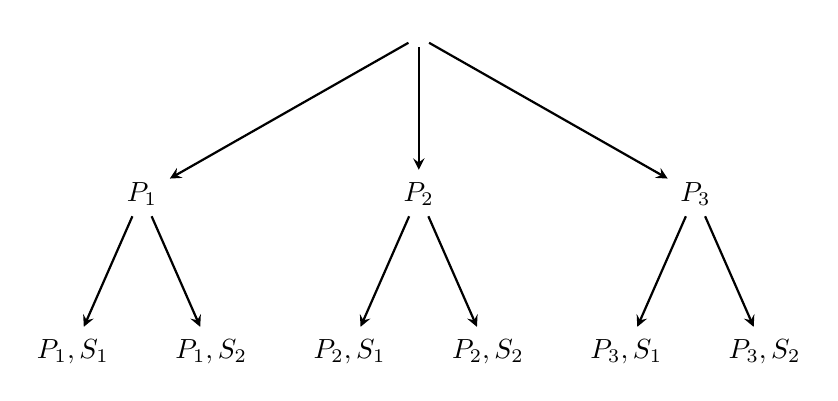
\begin{tikzpicture}[->,>=stealth,shorten >=1pt,auto,node distance=2cm,thick,main node/.style={scale=0.85,circle,draw,font=\sffamily\normalsize}]
            \node[] (0) []{$\square$};
            \node[] (1) [below of = 0, xshift = -100]{$P_1$};
            \node[] (2) [below of = 0]{$P_2$};
            \node[] (3) [below of = 0, xshift = 100]{$P_3$};

            \node[] (4) [below of = 1, xshift = -25]{$P_1, S_1$};
            \node[] (5) [below of = 1, xshift = 25]{$P_1, S_2$};

            \node[] (6) [below of = 2, xshift = -25]{$P_2, S_1$};
            \node[] (7) [below of = 2, xshift = 25]{$P_2, S_2$};

            \node[] (8) [below of = 3, xshift = -25]{$P_3, S_1$};
            \node[] (9) [below of = 3, xshift = 25]{$P_3, S_2$};

            \path[every node/.style={font=\sffamily\small}]
                (0) edge (1)
                (0) edge (2)
                (0) edge (3)

                (1) edge (4)
                (1) edge (5)

                (2) edge (6)
                (2) edge (7)

                (3) edge (8)
                (3) edge (9)
                ;
        \end{tikzpicture}

        \caption{Ogni freccia rappresenta una scelta effettuabile. Ogni percorso, ossia una successione di frecce contigue, rappresenta una serie di scelte effettuate.}
    \end{figure}

    Questo tipo di grafico viene detto \textbf{albero}. Le frecce dell'albero vengono dette \textit{archi} ed esse connettono i vari \textit{nodi} dell'albero. Il nodo senza frecce entranti viene detto \textit{radice} dell'albero, mentre i nodi senza foglie uscenti vengono detti \textit{foglie} dell'albero -- in altre parole, bisogna immaginare l'albero come se fosse ribaltato. Notiamo come il numero di foglie dell'albero corrisponda esattamente al numero di pasti completi consumabili.

    Il ragionamento appena effettuato tramite l'albero viene comunemente definito come \textbf{principio moltiplicativo}: se posso scegliere un primo oggetto tra $m$ oggetti distinti e per ciascuna di queste scelte posso scegliere un secondo oggetto tra $n$ oggetti distinti, allora le scelte possibili sono $m \cdot n$. Il principio moltiplicativo è un principio estremamente intuitivo che permette di risolvere un numero sorprendente di problemi di conteggio, anche non banali.
    
    Notiamo inoltre come tale principio possa essere esteso ad un qualsiasi numero di scelte sequenziali utilizzando un ragionamento ad albero strutturato su più di due livelli. 
    \begin{enumerate}
        \item Supponiamo che nlla nostra hamburgeria preferita possiamo scegliere tra pane bianco o pane con sesamo, tra carne di manzo, di maiale o di pesce e tra ketchup, maionese, senape o salsa barbecue. I modi in cui possiamo scegliere un panino sono:
        \[2 \cdot 3 \cdot 3 = 18\]
        \item In Italia, una targa per autoveicoli è formata da una sequenza di 2 lettere, 3 cifre ed ulteriori 2 lettere. Assumendo di usare l'alfabeto latino $A, B, C, \ldots, Z$ e le cifre $0, 1, 2, \ldots, 9$, il numero di targhe che è possibile formare corrisponde a:
        \[26 \cdot 26 \cdot 10 \cdot 10 \cdot 10 \cdot 26 \cdot 26 = 26^2 \cdot 10^3 \cdot 26^2 = 456976000\]
    \end{enumerate}

    \begin{framedprinc}{Principio moltiplicativo}
        Se, in \( t \) passaggi successivi, si sceglie un oggetto tra \( m_1 \) oggetti distinti nel primo passaggio, un oggetto tra \( m_2 \) oggetti distinti nel secondo passaggio, e così via, fino al \( t \)-esimo passaggio con \( m_t \) oggetti distinti, il numero totale di scelte possibili è:
        \[m_1 \cdot m_2 \cdot \ldots \cdot m_t\]
    \end{framedprinc}

    Osserviamo come gli esempi visti precedentemente sono \textbf{statici}, ossia possiedono a priori una quantità conosciuta di elementi appartenenti ad ogni evento che non varia nel corso delle scelte effettuate. Nella maggior parte dei casi, tuttavia, tali informazioni dipendono dalla situazione proposta, facendo attenzione ai dati forniti dal problema. Facendo attenzione, il principio moltiplicativo, può essere applicato anche in casi in cui ci siano dei vincoli.

    Il caso tipico è quello di scelte consecutive di elementi presi dallo stesso insieme: se l'insieme di partenza ha $n$ elementi avrò $m_1 = n$ possibilità per la prima scelta, $m_2 = n-1$
    per la seconda, $m_3 = n - 3$ per la terza, e così via:
    \begin{enumerate}
        \item Supponiamo di trovarci alla stessa hamburgeria dell'esempio precedente. Questa volta, vogliamo ordinare un panino con due salse invece di una, a patto che le due salse siano distinte. I modi in cui possiamo scegliere un panino sono:
        \[2 \cdot 3 \cdot 3 \cdot (3-1) = 36\]

        \item Un'urna contiene 100 palline contrassegnate con i numeri $1, 2, 3, \ldots, 100$. Vogliamo estrarre in successione le palline dall'urna (dunque senza rimetterle in essa). Il numero di possibili ordini di estrazione corrisponde a:
        \[100 \cdot (100-1) \cdot (100-2) \cdot \ldots \cdot (100-98) \cdot (100-99) = 100! \approx 9.3326 \cdot 10^{157}\]
    \end{enumerate}

    In altre situazioni, invece, i vincoli potrebbero essere più articolati. Ad esempio, potremmo avere situazioni in cui alcuni elementi vengono esclusi solo in determinati casi. Ad esempio, consideriamo un alfabeto composto da $A, B, C, D, E$. Il numero di parole di 4 lettere che iniziano con la lettera $D$ può essere calcolato \curlyquotes{fissando} il fatto per la prima lettera si abbia una sola scelta possibile:
    \[1 \cdot 5 \cdot 5 \cdot 5 = 5^3\]

    Similmente, il numero di parole di 4 lettere che non iniziano con la lettera $D$ o la lettera $C$ è dato da:
    \[3 \cdot 5 \cdot 5 \cdot 5 = 3 \cdot 5^3\]

    Alcuni vincoli richiedono più attenzione, ma sono spesso riconducibili a vincoli più semplici. Ad esempio, supponiamo di voler calcolare il numero di parole di 4 lettere che non contengono due lettere consecutive identiche. Di primo occhio il problema sembra richiederci di calcolare a mano molte combinazioni. Notiamo però una via più semplice: per ogni scelta, ci basta considerare il fatto che avremo una possibilità in meno in quanto la lettera della scelta precedente è \curlyquotes{bloccata}:
    \[10 \cdot 9 \cdot 9 \cdot 9 = 10 \cdot 9^3\]
    
    \subsection{Principio additivo}

    Consideriamo ora una tipologia diversa di problema. In pasticceria ci sono 14 tipi di ciambelle e 16 tipi di muffin. Marco vuole comprare o una ciambella o un muffin (dunque non entrambi). Quante opzioni ha Marco? In tal caso, la risposta risulta semplice: $14 + 16 = 30$.

    Il principio applicato in questo caso è il \textbf{principio additivo}: abbiamo considerato i due insiemi di oggetti come se fossero un unico insieme, per poi contare il numero di scelte possibili. A differenza del principio moltiplicativo, affinché sia possibile applicare il principio additivo è necessario che una condizione sia soddisfatta: la \textbf{mutua esclusività}.

    \begin{frameddefn}{Mutua esclusività}
        Due eventi $A$ e $B$ sono detti mutualmente esclusivi se non possono accadere in contemporanea.
    \end{frameddefn}

    Nell'esempio precedente, la mutua esclusività era esplicitamente affermata nel problema. In situazioni più comuni, possiamo scomporre un problema di conteggio in più sotto-problemi ed utilizzare il principio additivo tra essi.
    
    Consideriamo ancora i modi di poter formare una targa in Italia (2 lettere, 2 cifre e 2 lettere). Vogliamo sapere qual è il numero di targe che contengono la lettera $P$ solo una volta. Proviamo a scomporre il problema nelle seguenti quattro sotto-tipologie di conteggio:
    \begin{itemize}
        \item \textit{Tipo 1:} targhe che contengono la lettera $P$ come prima lettera.
        \item \textit{Tipo 2:} targhe che contengono la lettera $P$ come seconda lettera.
        \item \textit{Tipo 3:} targhe che contengono la lettera $P$ come terza lettera.
        \item \textit{Tipo 4:} targhe che contengono la lettera $P$ come quarta lettera.
    \end{itemize}

    L'unione di queste quattro tipologie descrive correttamente il problema di conteggio iniziale. Tuttavia, le tipologie non sono mutualmente esclusive. Tale problematica deriva dall'imprecisa definizione delle tipologie stesse. Ad esempio, la definizione della prima tipologia non ci vieta di considerare al suo interno anche le targhe che contengono una $P$ sia come prima sia come seconda lettera. Dobbiamo quindi scomporre il problema in delle tipologie più precise:
    \begin{itemize}
        \item \textit{Tipo 1:} targhe che contengono la lettera $P$ \underline{solo} come prima lettera. Per questo tipo abbiamo $1 \cdot 25 \cdot 10^3 \cdot 25^2$ targhe.
        \item \textit{Tipo 2:} targhe che contengono la lettera $P$ \underline{solo} come seconda lettera. Per questo tipo abbiamo $25 \cdot 1 \cdot  10^3 \cdot 25^2$ targhe.
        \item \textit{Tipo 3:} targhe che contengono la lettera $P$ \underline{solo} come terza lettera. Per questo tipo abbiamo $25^2 \cdot 10^3 \cdot 1 \cdot 25$ targhe.
        \item \textit{Tipo 4:} targhe che contengono la lettera $P$ \underline{solo} come quarta lettera. Per questo tipo abbiamo $25^2 \cdot 10^3 \cdot 25 \cdot 1$ targhe.
    \end{itemize}

    Tramite la nuova definizione, i quattro eventi sono mutualmente esclusivi. Per tanto, possiamo applicare il principio additivo tra essi:
    \[T_1 + T_2 + T_3 + T_4 = 4 \cdot 25^3 \cdot 10^3\]

    \begin{framedprinc}{Principio additivo}
        Se un'azione può essere eseguita in uno dei $m_1$ modi e in modo alternativo può essere eseguita in $m_2$ modi, e così via, fino a $m_t$ modi distinti e \underline{mutualmente esclusivi}, allora il numero totale di modi possibili di eseguire l'azione è:
        \[m_1 + m_2 + \ldots + m_t\]
    \end{framedprinc}

    \subsection{Principio di inclusione-esclusione}

    Supponiamo di dover contare quante siano le targhe contenenti nessuna $T$ o nessun $9$ al loro interno. Effettuare una tipizzazione disambigua e completa di questo insieme richiederebbe chiaramente troppo tempo poiché sarebbe richiesto di gestire tutti i vari sotto-casi.

    Per risolvere problemi di conteggio come questo, è sufficiente utilizzare le regole dell'insiemistica. Difatti, fino ad ora abbiamo trattato i problemi di conteggio come semplici quantità. Tuttavia, è più opportuno considerare tali problemi come il calcolo della \textbf{cardinalità} dell'insieme descrivente il problema. 
    
    Sia quindi $\text{Non-T-o-9}$ l'insieme delle targhe contenenti nessuna $T$ o nessun $9$ al loro interno. Per risolvere il problema è sufficiente calcolare $\abs{\text{Non-T-o-9}}$, ossia la cardinalità di $\text{Non-T-o-9}$. Utilizziamo quindi l'insiemistica per scomporre il problema. Sia $\text{Non-T}$ l'insieme delle targhe contenenti nessuna $T$ e sia $\text{Non-9}$ definito analogamente per 9. Abbiamo che:
    \[\text{Non-T-o-9} = \text{Non-T} \cup \text{Non-9}\]

    Contrariamente a quanto si possa pensare di primo getto, abbiamo che:
    \[\abs{\text{Non-T} \cup \text{Non-9}} \neq \abs{\text{Non-T}} + \abs{\text{Non-9}}\]
    
    Per capire il perché di tale non-uguaglianza, consideriamo il diagramma di Venn descrivente il problema:
    \begin{figure}[H]
        \centering

        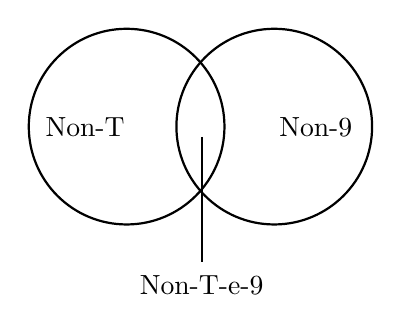
\begin{tikzpicture}[-,>=stealth,shorten >=1pt,auto,node distance=0.25cm,thick,main node/.style={scale=0.85,circle,draw,font=\sffamily\normalsize}]
            \node[draw, circle, scale=7.5] (0) []{};
            \node[draw, circle, scale=7.5] (1) [right of = 0]{};

            \node[] (2) [at = {(0)}, xshift = -15]{Non-T};
            \node[] (3) [at = {(1)}, xshift = 15]{Non-9};
            \node[] (4) [right of = 0, xshift = 20]{};
            \node[] (5) [below of = 4, yshift = -50]{Non-T-e-9};

            \path[every node/.style={font=\sffamily\small}]
                (4) edge (5)
                ;
        \end{tikzpicture}

        \caption{Diagramma di Venn per l'insieme Non-T-o-9}
    \end{figure}

    Sommando le due cardinalità $\abs{\text{Non-T}}$ e $\abs{\text{Non-9}}$ stiamo quindi sommando \underline{due volte} la cardinalità $\abs{\text{Non-T-e-9}}$. Per poter bilanciare i conti, è necessario sottrarre una volta tale cardinalità dal conteggio, ottenendo che:
    \[\begin{split}
        \abs{\text{Non-T} \cup \text{Non-9}} &= \abs{\text{Non-T}} + \abs{\text{Non-9}} - \abs{\text{Non-T-e-9}}\\
        &= 25^2 \cdot 10^3 \cdot 25^2 + 26^2 \cdot 9^3 \cdot 26^2 - 25^2 \cdot 9^3 \cdot 25^2 \\
        &= 25^4 \cdot 10^3 + 26^4 \cdot 9^3 - 25^4 \cdot 9^3
    \end{split}\]

    Tale fatto è noto in insiemistica come \textbf{principio di inclusione-esclusione}.

    \begin{framedprinc}{Principio di inclusione-esclusione}
        Dati due insiemi $A$ e $B$, si ha che:
        \[\abs{A \cup B} = \abs{A} + \abs{B} - \abs{A \cap B}\]
    \end{framedprinc}

    In particolare, poniamo maggior attenzione al modo in cui il principio di inclusione-esclusione sia generalizzato ad un numero qualsiasi di insiemi. Consideriamo una classe di
    41 studenti sottoposti a tre test di valutazione: Algebra (A), Basi di dati (B) e Calcolo delle probabilità (C). I risultati dei test a nostra disposizione sono i seguenti: 12 studenti superano A, 5 studenti superano B, 8 studenti superano C, 2 studenti superano sia A che B, 6 studenti superano sia A che C, 3 studenti superano sia B che C, 1 studente supera sia A che B che C. Vogliamo sapere quanti studenti hanno superato almeno un test. Come nell'esempio precedente, descriviamo il problema tramite un diagramma di Venn:

    \begin{figure}[H]
        \centering

        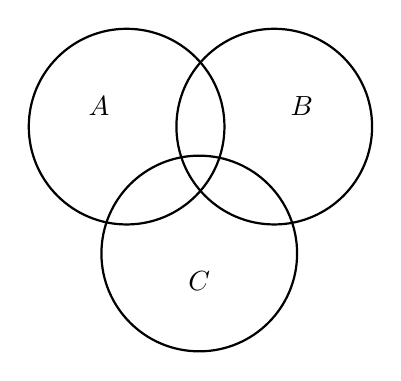
\begin{tikzpicture}[-,>=stealth,shorten >=1pt,auto,node distance=0.25cm,thick,main node/.style={scale=0.85,circle,draw,font=\sffamily\normalsize}]
            \node[draw, circle, scale=7.5] (0) []{};
            \node[draw, circle, scale=7.5] (1) [right of = 0]{};
            \node[draw, circle, scale=7.5] (2) [below of = 0, xshift = 3.5, yshift = 1]{};

            \node[] (x) [at = {(0)}, xshift = -10, yshift=7.5]{$A$};
            \node[] (x) [at = {(1)}, xshift = 10, yshift=7.5]{$B$};
            \node[] (x) [at = {(2)}, yshift = -10]{$C$};

            \path[every node/.style={font=\sffamily\small}]
                ;
        \end{tikzpicture}

        \caption{Diagramma di Venn per il problema delle verifiche.}
    \end{figure}
    
    Sommando le tre cardinalità $\abs{A}, \abs{B}$ e $\abs{C}$, ciascuna delle cardinalità $\abs{A \cap B}, \abs{A \cap C}$ e $\abs{B \cap C}$ viene sommata due volte. Per controbilanciare, dobbiamo sottrarre ciascuna di esse almeno una volta. Tuttavia, così facendo la cardinalità $\abs{A \cap B \cap C}$ è stata sommata tre volte e sottratta tre volte. Per controbilanciare nuovamente, dobbiamo sommare essa una volta, ottenendo quindi:
    \[\begin{split}
        \abs{A \cup B \cup C} &= \abs{A} + \abs{B} + \abs{C} - \abs{A \cap B} - \abs{A \cap C} - \abs{B \cap C} + \abs{A \cap B \cap C} \\
        &= 12 + 5 + 8 - 2 - 6 - 3 + 1 \\
        &= 15
    \end{split}\]

    Per rendere il ragionamento più meccanico (togliendo anche di mezzo il diagramma di Venn), possiamo applicare ripetutamente il principio di inclusione-esclusione tra due insiemi:
    \[\begin{split}
        \abs{A \cup B \cup C} & = \abs{(A \cup B) \cup C} \\
        &= \abs{A \cup B} + \abs{C} - \abs{(A \cup B) \cap C}  \\
        & = \abs{A \cup B} + \abs{C} - \abs{(A \cap C) \cup (B \cap C)} \\
        & = (\abs{A} + \abs{B} - \abs{A \cap B}) + \abs{C} - (\abs{A \cap B} + \abs{B \cap C} - \abs{(A \cap C) \cap (B \cap C)}) \\
        & =  \abs{A} + \abs{B} + \abs{C} - \abs{A \cap B} - \abs{A \cap C} - \abs{B \cap C} + \abs{A \cap B \cap C}
    \end{split}\]

    Un ulteriore appunto da fare riguarda come il principio additivo sia in realtà un \textit{sotto-caso} del principio di inclusione esclusione. Difatti, due eventi $A$ e $B$ sono mutualmente esclusivi se e solo se $A \cap B = \varnothing$. Se tutti gli eventi $A_1, \ldots, A_n$ coinvolti sono mutualmente esclusivi, dunque $A_i \cap A_j = \varnothing$ per ogni $i,j \in \{1, \ldots, n\}$, le cardinalità di tutte le intersezioni coinvolte nel principio di inclusione-esclusione sono nulle, degenerando quindi nel principio additivo. Quando ciò si verifica, gli insiemi coinvolti vengono detti \textbf{partizione}.
    
    \label{partizione}
    \begin{frameddefn}{Partizione}
        Dato un insieme $A$, gli insiemi $A_1, \ldots, A_n$ vengono detti partizione di $S$ quando:
        \begin{itemize}
            \item Ognuno degli insiemi è sottoinsieme di $S$, ossia $A_i \subseteq A$ per ogni $i \in \{1, \ldots, n\}$
            \item Gli insiemi sono due a due disgiunti, ossia $A_i \cap A_j = \varnothing$ per ogni $i,j \in \{1, \ldots, n\}$
            \item L'unione degli insiemi è uguale ad $S$, ossia $A = A_1 \cup \ldots \cup A_n$
        \end{itemize}
    \end{frameddefn}

    \begin{figure}[H]
        \centering
        \includegraphics[scale=0.3]{images/partizione.png}
        \caption{Rappresentazione grafica di una partizione}
    \end{figure}

    \subsection{Passaggio al complemento}

    Vediamo ora l'ultimo strumento fondamentale alla base dei conteggi. Supponiamo di voler contare quante siano le targhe contenenti almeno una $T$. Calcolare tale quantità tramite il principio additivo, o più generalmente tramite il principio di inclusione-esclusione, richiederebbe di enumerare (ossia \curlyquotes{listare}) una lunga quantità di sotto-tipi che possano descrivere il problema comodamente. In questo caso, è più efficiente effettuare quello che viene chiamato \textbf{passaggio al complemento}. Dato un insieme $A \subseteq S$, il complemento di $A$, indicato come $\overline{A}$ o come $S - A$, è l'insieme di tutti gli elementi di $S$ che non si trovano in $A$:
    \[\overline{A} = S- A = \{x \in S \mid x \notin A\}\]

    Per definizione, notiamo che un insieme $A$ e il suo complemento $\overline{A}$ costituiscono \textit{sempre} una partizione dell'insieme totale $S$ che li contiene. Per tanto, tramite il principio additivo abbiamo che:
    \[\abs{S} = \abs{A} + \abs{\overline{A}} \implies \abs{A} = \abs{S} - \abs{\overline{A}}\]

    \begin{framedprinc}{Passaggio al complemento}
        Dato un insieme $A \subseteq S$, si ha che:
        \[\abs{A} = \abs{S} - \abs{\overline{A}}\]
    \end{framedprinc}

    Nel nostro esempio, il complemento dell'insieme $A$ contenente tutte le targhe aventi almeno una $T$ corrisponde all'insieme $\overline{A}$ contenente tutte le targhe senza alcuna $T$, mentre l'insieme $S$ corrisponde all'insieme di tutte le targhe possibili. Abbiamo quindi che:
    \[\abs{A} = \abs{S} - \abs{\overline{A}} = 26^2 \cdot 10^3 \cdot 26^2 - 25^2 \cdot 10^3 \cdot 25^2\]

    Tra tutti gli strumenti visti fino ad ora, il passaggio al complemento risulta essere uno dei più potenti, permettendoci di rendere banali problemi che altrimenti sarebbero complessi. Tuttavia, come disse lo zio Ben, \curlyquotes{da un grande potere derivano grandi responsabilità}: applicare il passaggio al complemento in modo corretto non è un'operazione così immediata. Difatti, è sempre opportuno assicurarsi che l'insieme descrivente il complemento di ciò che cerchiamo sia effettivamente giusto.
    
    Ad esempio, immaginiamo di dover contare quante siano le targhe contenenti almeno una $T$ e almeno
    un $9$ al loro interno. Di primo occhio, potremmo pensare che il complemento di tale richiesta sia l'insieme delle targhe che non contengono nessuna $T$ \underline{e} nessun $9$. Tuttavia, ciò è sbagliato. Per capire il motivo, immaginiamo il concetto di complemento come l'apposizione di un'etichetta contrassegnata con \curlyquotes{non è vero che} davanti alla nostra affermazione originale. A questo punto, notiamo che l'affermazione \curlyquotes{non è vero che ho svolto sia $A$ che $B$} è equivalente all'affermazione \curlyquotes{non ho svolto $A$ oppure non ho svolto $B$}. Difatti, il complemento della richiesta iniziale corrisponde all'insieme delle targhe che non contengono nessuna $T$ \underline{o} nessun $9$.
    \[\begin{split}
        \abs{\text{Almeno-una-T-e-Almeno-un-9}} &= \abs{\text{Targhe}} - \abs{\text{Non-T-o-Non-9}} \\
        &= 26^2 \cdot 10^3 \cdot 26^2 - (25^4 \cdot 10^3 + 26^4 \cdot 9^3 - 25^4 \cdot 9^3)
    \end{split}\]
    
    In insiemistica e logica, tale concetto è noto come primo \textbf{teorema di De Morgan}. Il secondo teorema, invece, afferma che \curlyquotes{non è vero che ho svolto $A$ o $B$} è equivalente all'affermazione \curlyquotes{non ho svolto $A$ e non ho svolto $B$}.

    \begin{framedthm}{Teoremi di De Morgan}
        Dati gli insiemi $A_1, \ldots, A_n$, si ha che:
        \[\overline{A_1 \cup \ldots \cup A_n} = \overline{A_1} \cap \ldots \cap \overline{A_n}\]
        \[\overline{A_1 \cap \ldots \cap A_n} = \overline{A_1} \cup \ldots \cup \overline{A_n}\]
    \end{framedthm}

    \begin{proof}
        Omessa.
    \end{proof}

    Nonostante la sua potenza, non sempre il passaggio al complemento risulta essere la via migliore. Ciò accade soprattutto quando calcolare il complemento è difficile quanto calcolare il problema iniziale (se non addirittura più difficile). Consideriamo il seguente esempio. In una gara di 8 atleti di cui 2 italiani, 3 francesi e 3 spagnoli, vogliamo sapere quanti sono gli ordini di arrivo
    in cui i primi tre atleti hanno nazionalità diverse. Sia quindi $A$ l'insieme degli ordini di arrivo con i tre primi posti occupati da atleti di nazionalità diverse. Per calcolare tale quantità tramite il principio additivo, possiamo suddividere il problema in sei sotto-casi mutualmente esclusivi:
    \begin{itemize}
        \item $IFS$ è l'insieme degli ordini di arrivo con un italiano primo, un francese secondo e uno spagnolo terzo
        \item $ISF$ è l'insieme degli ordini di arrivo con un italiano primo, uno spagnolo secondo e un francese terzo
        \item $FIS$ è $\ldots$
        \item $FSI$ è $\ldots$
        \item $SIF$ è $\ldots$
        \item $SFI$ è $\ldots$
    \end{itemize}

    Questi sei sottoinsiemi sono una corretta partizione dell'insieme $A$ ma richiedono un numero di calcoli elevato. Tuttavia, non possiamo fare di meglio: il complemento della richiesta in questo caso corrisponderebbe all'insieme contenente gli ordini di arrivo con due posizioni occupate dalla stessa nazionalità. Calcolare tale complemento richiederebbe un numero di casi persino superiore alla richiesta iniziale (ad esempio, abbiamo nove casi suddividendoli in \curlyquotes{italiani primi e secondi, italiani primi e terzi, italiani secondi e terzi, francesi primi e secondi, $\ldots$}).
    
    Per tanto, calcoliamo i vari sei casi. Per il caso $IFS$, per la prima posizione abbiamo 2 scelte, per la seconda 3 e per la terza altre 3. Per tutte le posizioni rimanenti, possiamo considerare tutti i corridori indipendentemente dalla loro nazione, avendo quindi 5 scelte per la quarta posizione, 4 per la quinta, e così via. Abbiamo quindi che $\abs{IFS} = 2 \cdot 3 \cdot 3 \cdot 5!$. Per tutti gli altri casi, possiamo procedere in modo analogo, ottenendo che:
    \[\begin{split}
        \abs{A} &= \abs{IFS} + \abs{ISF} + \abs{FIS} + \abs{FSI} + \abs{SIF} + \abs{SFI} \\
        &= 6 \cdot 2 \cdot 3^2 \cdot 5!
    \end{split}\]

    \section{Figure della combinatoria}

    \subsection{Disposizioni}

    Una volta compresi i due principi alla base del calcolo combinatorio, di seguito vedremo anche quelle che sono le figure fondamentali del calcolo combinatorio, ossia casistiche estremamente ricorrenti nel calcolo combinatorio. La prima figura combinatoria che analizzeremo sono le \textbf{disposizioni}. Una disposizione è un ordinamento di $k$ oggetti presi da un insieme di $n$. La caratteristica fondamentale di una disposizione è che l'ordine degli oggetti conta (ossia vi è distinzione tra la parola $APE$ e la parola $AEP$). In particolare distinguiamo in due tipologie di disposizioni:
    \begin{itemize}
        \item \textbf{Disposizioni con ripetizione}: gli elementi già scelti possono essere nuovamente scelti -- dunque come se venissero reinseriti nel sacchetto da cui vengono estratti.
        \item \textbf{Disposizioni semplici}: dopo ogni scelta il numero di elementi tra cui scegliere decrementa di uno -- dunque come se venissero rimossi del tutto dal sacchetto da cui vengono estratti.
    \end{itemize}

    \begin{frameddefn}{Disposizione}
        Dati due interi $n, k > 0$, definiamo:
        \begin{itemize}
            \item Le disposizioni con ripetizioni di $n$ oggetti su $k$ posizioni, indicate con $D'_{n,k}$, come le sequenze ordinate di $k$ oggetti scelti tra gli $n$ totali
            \item Le disposizioni semplici di $n$ oggetti su $k$ posizioni, indicate con $D_{n,k}$, come le sequenze ordinate di $k$ oggetti \underline{distinti} scelti tra gli $n$ totali
        \end{itemize}
    \end{frameddefn}

    Consideriamo l'alfabeto composto da $a, b, c, d, e$. Vogliamo contare le sequenze ordinate di lunghezza 2 di lettere scelte nell'alfabeto dato, con possibili ripetizioni tra di esse. Usando il principio moltiplicativo, il numero di disposizioni corrisponde a $5 \cdot 5 = 5^2$. Similmente, il numero di sequenze ordinate di lunghezza 7 con ripetizioni è dato da $5^7$. Notiamo quindi la presenza di un pattern: dati $n,k > 0$, il numero di disposizioni con ripetizione è $D'_{n,k} = n^k$.
    
    Se volessimo calcolare le sequenze ordinate di lunghezza 2 senza ripetizioni, invece, usando il principio moltiplicativo abbiamo $5 \cdot 4$ disposizioni semplici. Se invece considerassimo quelle di lunghezza 3, invece, avremmo $5 \cdot 4 \cdot 3$ disposizioni. Anche in questo caso, notiamo un pattern. Per il primo caso, abbiamo esattamente $\frac{5!}{(5-2)!}$ disposizioni, mentre per il secondo abbiamo $\frac{5!}{(5-3)!}$ disposizioni. Per quelle di lunghezza 7 invece, notiamo come il numero di lettere sia insufficiente: non potremo mai avere una sequenza ordinata di 7 lettere se il numero di lettere è minore di 7. Per tanto, in tal caso la risposta risulta essere 0.

    \begin{framedprop}{Conteggio delle disposizioni}
        Dati due interi $n, k > 0$, il numero di disposizioni con ripetizione su $k$ posizioni scelte tra $n$ oggetti è dato da:
        \[D'_{n,k} = n^k\]

        Per le disposizioni senza ripetizione, invece, abbiamo che:
        \[D_{n,k} = \soe{ll}{
            \frac{n!}{(n-k)!} & \text{se } k \leq n\\
            0 & \text{altrimenti} \\
        }\]
    \end{framedprop}

    Supponiamo che ad un torneo partecipino 8 squadre scelte tra 15 squadre iscritte. Sapendo che l'ordine di partenza è estratto a sorte, vogliamo calcolare i possibili ordini di partenza. In questo caso è immediato notare come ci troviamo in una disposizione semplice. Per tanto, la risposta risulta immediata:
    \[\frac{15!}{(15-8)!} = \frac{15!}{7!} = 15 \cdot 14 \cdot \ldots \cdot 8\]
    
    Se invece tutte le squadre possono partecipare al torneo, in tal caso il numero di ordini di partenza possibile è dato da:
    \[\frac{15!}{(15-15)!} = \frac{15!}{0!} = 15!\]

    Notiamo quindi come nel caso particolare in cui il numero di posizioni da disporre coincide con il numero di elementi a disposizione, le disposizioni semplici $D_{n,n}$ corrispondono esattamente al numero in cui è possibile ordinare gli $n$ elementi. Questo particolare tipo di disposizione semplice viene detta \textbf{permutazione}.

    \begin{frameddefn}{Permutazioni}
        Dato un intero $n > 0$, definiamo le permutazioni di $n$ elementi, indicate con $P_n$, come tutti i possibili ordinamenti di $n$. In altre parole $P_n = D_{n,n}$.
    \end{frameddefn}

    Non sempre il problema è posto in termini espliciti che rimandano alle disposizioni. Ad esempio, consideriamo il problema di contare in quanti modi posso inserire esattamente una $P$ ed esattamente una $R$ in una targa (\textit{Attenzione}: ciò non equivale a chiedere il numero di targhe contenenti esattamente una $P$ ed esattamente una $R$). Il problema può essere ricondotto alle disposizioni semplici se osserviamo che esso equivalga a contare le coppie ordinate di possibili posizioni occupate dalle due lettere. Più precisamente, gli oggetti che vogliamo contare sono le coppie ordinate $(i, j)$ con $i \neq j$ e $i, j \in \{1, 2, 6, 7\}$, ossia le posizioni occupabili dalle lettere nella targa. Ogni coppia $(i, j)$ corrisponde a una targa in cui mettiamo $P$ in posizione $i$ e $R$ in posizione $j$. Si tratta dunque di disposizioni semplici di $2$ elementi (le posizioni occupate) scelte tra 4 oggetti (le posizioni possibili), ossia $D_{4,2} = \frac{4!}{2!} = 4 \cdot 3$.

    \subsection{Anagrammi}

    Gli \textbf{anagrammi} sono una generalizzazione del concetto di disposizione semplice. Per capire intuitivamente diretto di cosa tratta, cerchiamo di calcolare il numero di anagrammi della parola NONNA.
    Nel caso in cui considerassimo ognuna delle lettere ripetute come una lettera diversa (quindi come se la parola in questione fosse $N_1 O N_2 N_3 A$), potremmo identificare la risposta come una semplice permutazione di tutte le lettere disponibili, quindi $P_5 = 5! = 120$.
        
    Nel caso in cui invece considerassimo le lettere ripetute come la stessa, avremmo degli anagrammi uguali tra loro poiché le tre N sono intercambiabili tra loro. In questo caso, quindi, sarà necessario dividere il numero di permutazioni originali per il numero di permutazioni della quantità $n_1$ di lettere N ripetute
    \[\frac{P_n}{P_{n_1}} = \frac{P_5}{P_3} = \frac{5!}{3!} = 20\]

    Per quanto riguarda gli anagrammi della parola NONNO, ci troviamo in una situazione molto simile alla precedente. Tuttavia le tipologie di lettere ripetute sono ora due: N ed O. Per soddisfare la domanda, possiamo procedere con lo stesso metodo, dividendo il numero delle permutazioni originali per il numero delle permutazioni della quantità di lettere N ripetute e di lettere O ripetute, che chiameremo rispettivamente \textit{$n_1$} e \textit{$n_2$}.
    \[\frac{P_n}{P_{n_1} \cdot P_{n_2}} = \frac{P_5}{P_3 \cdot P_2} = \frac{5!}{3! \cdot 2!} = 10\]
    
    Ricapitolando, per ottenere il numero di anagrammi di una parola formata da \textit{n occorrenze} di lettere di cui $n_1$ sono identiche, allora avremo $\frac{n!}{n_1!}$ possibilità. Nel caso in cui ci siano $n_1$ lettere identiche di un tipo e $n_2$ di un altro tipo, allora avremo $\frac{n!}{n_1! \cdot n_2!}$ possibilità. Lo stesso ragionamento può essere applicato con parole in cui compaiono $t$ gruppi di $n_1, n_2, ..., n_t$.

    \begin{framedprop}{Conteggio degli anagrammi}
        Data una parola lunga $n$ lettere in cui compaiono $t$ gruppi di $n_1, ..., n_t$ lettere ripetute, con $0 \leq n_1 + \ldots + n_t \leq n$, il numero di anagrammi della parola è dato da:
        \[A_{n,n_1,\ldots, n_t} = \frac{n!}{n_1! \cdot n_2! \cdot ... \cdot n_t!}\]
    \end{framedprop}
    
    Il calcolo degli anagrammi, tuttavia, non si limita ad essere applicato solo nel caso in cui sia lavori con parole, bensì in qualsiasi problema analogo dove ogni tipologia di elemento può essere associata ad una lettera. Ad esempio, possiamo utilizzare gli anagrammi per rispondere alla seguente domanda: quanti sono gli ordinamenti di 14 frutti di cui 7 mele e 3 pere e 4 pesche se mi interessa soltanto distinguere tra mele, pere e banane? Difatti, risponde a tale domanda equivale a calcolare il numero di anagrammi di una parola contenente 7 $M$, 3 $P$ e 4 $B$.
    \[A_{14,7,3,4} = \frac{14!}{7! \cdot 3! \cdot 4!} = 120120\]

    \subsection{Combinazioni}

    Fino ad ora, abbiamo visto problemi in cui veniva sempre considerato l'\textit{ordine} in cui gli elementi si presentavano gli elementi di un dato insieme (permutazioni e disposizioni). Nell'ambito delle \textbf{combinazioni}, invece, l'ordine non ha alcuna importanza.
    
    \begin{frameddefn}{Combinazione}
        Dati due interi $n,k >0 $, una combinazione di $k$ oggetti presi dagli $n$ totali è sequenza non-ordinata di $k$ elementi \underline{distinti} scelti tra gli $n$ totali
    \end{frameddefn}

    Per capire meglio di cosa si tratta, vediamo il seguente esempio.
    Consideriamo l'insieme $A = \{a,b,c,d\}$. Vogliamo contare quante sono le parole formate da 3 caratteri distinti di $A$, senza tener conto del loro ordine di occorrenza. Ad esempio, per i tre caratteri $a,b,c$ vogliamo assumere che:
    \[ abc = acb = bac = bca = cab = cba\]
        
    Possiamo quindi facilmente contare manualmente quanti siano le stringhe distinte non ordinate possibili, ossia $abc, abd, acd, bcd$. Per poter calcolare tali combinazioni in modo più strutturato, possiamo ricavare il concetto partendo dalle disposizioni semplici. Per 4 elementi e 3 posizioni, abbiamo che: 
    \[D_{4,3} = \frac{4!}{(4-3)!} = 4! = 16\]

    Proviamo quindi a listare tutte le disposizioni semplici date dal problema, raggruppandole in base agli elementi che compaiono in esse:
    \begin{itemize}
        \item Abbiamo $3!$ disposizioni semplici contenenti $a,b$ e $c$
        \[abc, acb, bac, bca, cab, cba\]
        \item Abbiamo $3!$ disposizioni semplici contenenti $a,b$ e $d$
        \[abd, adb, bad, bda, dab, dba\]
        \item Abbiamo $3!$ disposizioni semplici contenenti $a,c$ e $d$
        \[adc, acd, dac, dca, cad, cda\]
        \item Abbiamo $3!$ disposizioni semplici contenenti $b,c$ e $d$
        \[dbc, dcb, bdc, bcd, cdb, cbd\]
    \end{itemize}

    Una volta enumerate tutte le possibili disposizioni semplici, possiamo notare come, considerando il caso in cui l'ordine non sia importante, ogni gruppo corrisponda allo \textit{stesso sottoinsieme}. Per ottenere la quantità di combinazioni semplici, dunque, sarà necessario considerare solo \textit{1 disposizione} per gruppo. In altre parole, abbiamo solo 4 sottoinsiemi possibili.    Per tradurre in formula questo concetto, quindi, è necessario dividere la disposizione semplice $D_{4, 3}$ per $3!$, ossia il numero di elementi in ogni gruppo:
    \[\frac{\dfrac{4!}{(4-3)!}}{3!} = \frac{4!}{(4-3)! \cdot 3!} = 4\]

    Questo particolare risultato può essere riscritto più compattamente tramite il \textbf{coefficiente binomiale} $\binom{4}{3}$ letto come \curlyquotes{4 scelgo 3}. Difatti, in combinatoria, il coefficiente binomiale $\binom{n}{k}$ rappresenta esattamente i modi di scegliere $k$ elementi da un insieme di $n$ elementi, senza dare importanza all'ordine.

    \begin{framedprop}{Calcolo delle combinazioni}
        Dati due interi $n, k$, con $0 \leq k \leq n$, il numero di combinazioni semplici di $k$ elementi scelti tra $n$ oggetti corrisponde a:
        \[C_{n,k} = \binom{n}{k} = \frac{n!}{(n-k)! \cdot k!}\]
    \end{framedprop}
    
    Per prendere confidenza con le combinazioni semplici (e dunque con i coefficienti binomiali), vediamo alcuni esempi. In un'azienda di 80 individui, vogliamo scegliere una delegazione di rappresentati.
    
    \begin{enumerate}
        \item In quanti modi possiamo formare una delegazione di 4 rappresentanti? Questo è un tipico esempio di applicazione diretta del concetto di combinazione semplice, poiché non ci interessa l'ordine dei rappresentanti della delegazione. Se $A$ è l'insieme descrivente la richiesta, abbiamo che:
        \[\abs{A} = C_{80,4} = \binom{80}{4} = \frac{80!}{(80-4)! \cdot 4!} = \frac{80 \cdot 79 \cdot 78 \cdot 77}{4 \cdot 3 \cdot 2 \cdot 1}\]
                   
        \item Assumendo che gli 80 individui siano divisi tra 30 maschi e 50 femmine, quante sono le delegazioni con 2 individui per entrambi i sessi? In questo caso, possiamo calcolare le totali combinazioni possibili calcolando prima le combinazioni possibili per scegliere i due componenti maschili e successivamente le combinazioni per scegliere quelli femminili, per poi calcolare il prodotto di entrambe applicando il principio moltiplicativo. Se $B$ è l'insieme descrivente la richiesta, abbiamo che:
        \[\abs{B} = \binom{30}{2} \cdot \binom{50}{2}\]
            
        \item Assumendo sempre che gli 80 individui siano divisi tra 30 maschi e 50 femmine, quante sono le delegazioni di 4 individui con almeno un rappresentante per ogni sesso? La parola chiave \textit{almeno} indica la possibilità di ottenere la risposta attraverso un \textit{passaggio al complemento}. Usando il teorema di De Morgan, il complemento della richiesta corrisponde all'insieme delle delegazioni con solo rappresentanti maschi o solo rappresentanti femmine. Essendo i due eventi mutualmente esclusivi tra loro (non può esserci una delegazione con solo maschi ed una con solo femmine). Se $C$ è l'insieme descrivente la richiesta, abbiamo che:
        \[\abs{C} = \binom{80}{4} - \binom{30}{2} - \binom{50}{2}\]
            
        \item Quanti modi abbiamo di scegliere una delegazione di 4 rappresentanti in cui un membro assume il ruolo di portavoce? In questo caso, possiamo prima scegliere prima il portavoce e successivamente gli altri 3 rappresentanti. Se $D$ è l'insieme descrivente la richiesta, abbiamo che:
        \[\abs{D} = \binom{80}{1} \cdot \binom{79}{3}\]
    \end{enumerate}

    Consideriamo ora un insieme $A = \{a_1, \ldots, a_n\}$ contenente $n$ elementi. Osserviamo che il concetto di combinazione può essere utilizzato anche per calcolare il numero di  sottoinsiemi $B_1, \ldots, B_m$ ciascuno contenente $k$ elementi scelti da $A$. Difatti, all'interno di un insieme non possono esserci elementi ripetuti e l'ordine degli elementi non è importante. Per tanto, tra gli $n$ elementi ci interessa solo sceglierne $k$, senza contare il loro ordine di occorrenza, dunque il numero $m$ di sottoinsiemi corrisponde ai modi di scegliere i $k$ elementi. Ad esempio, dato $A = \{a,b,c,d\}$, il numero di sottoinsiemi contenenti $2$ elementi è dato da:
    \[\binom{4}{2} = \frac{4!}{2! \cdot 2!} = \frac{4 \cdot 3}{2} = 6\]

    Difatti, tali sottoinsiemi corrispondono a $\{a,b\}, \{a,c\}, \{a,d\}, \{b,c\}, \{b,d\}, \{c,d\}$.

    \begin{framedprop}{Conteggio di sottoinsiemi}
        Dato un insieme $A$ con $n$ elementi, il numero di sottoinsiemi di $A$ contenenti $k$ elementi corrisponde al numero di combinazioni di $k$ elementi scelti dagli $n$ totali, ossia $\binom{n}{k}$
    \end{framedprop}

    \subsection{Proprietà dei coefficienti binomiali}

    Nella sezione precedente, abbiamo discusso quali siano i modi di scegliere una delegazione di 4 rappresentanti scelti tra 80 individui, dove un membro della delegazione assume il ruolo di portavoce. Scegliendo prima il portavoce e successivamente gli altri 3 rappresentati, abbiamo visto che tale numero di delegazioni corrisponde a:
    \[\binom{80}{1} \binom{79}{3} = \frac{80!}{1! \cdot 79!} \cdot \frac{79!}{3! \cdot 76!} = 80 \cdot \frac{79 \cdot 78 \cdot 77}{3 \cdot 2 \cdot 1} = \frac{80 \cdot 79 \cdot 78 \cdot 77}{3 \cdot 2}\]

    \newpage

    Tuttavia, per trovare tale quantità avremmo potuto anche ragionare nel seguente modo: scegliamo prima i 4 rappresentati e poi tra di essi scegliamo un portavoce. Difatti, notiamo che:
    \[\binom{80}{4} \binom{4}{1} = \frac{80!}{4! \cdot 76!} \cdot \frac{4!}{1! \cdot 3!} = \frac{80 \cdot 79 \cdot 78 \cdot 77}{4 \cdot 3 \cdot 2 \cdot 1} \cdot 4 = \frac{80 \cdot 79 \cdot 78 \cdot 77}{3 \cdot 2}\]

    Difatti, più in generale vale la seguente identità.

    \begin{framedprop}{}
        Dati tre interi $n,m,k \in \N$ tali che $0 < k \leq m \leq n$, si ha che:
        \[\binom{n}{m} \binom{m}{k} = \binom{n}{k} \binom{n-k}{m-k}\]
    \end{framedprop}

    \begin{proof}
        Tramite un po' di manipolazione algebrica abbiamo che:
        \[\begin{split}
            \binom{n}{k} \binom{n-k}{m-k} &= \frac{n!}{k! \cdot (n-k)!} \cdot \frac{(n-k)!}{(m-k)! \cdot (n-k - (m-k))!} \\
            &= \frac{n!}{k!} \cdot \frac{1}{(m-k)! \cdot (n-m)!} \\
            &= \frac{n!}{k!} \cdot \frac{1}{(m-k)! \cdot (n-m)!} \cdot \frac{m!}{m!}\\
            &= \frac{n!}{m! \cdot (n-m)!} \cdot \frac{m!}{k! \cdot (m-k)!}\\
            &= \binom{n}{m} \binom{m}{k}
        \end{split}\]
    \end{proof}

    I coefficienti binomiali godono di molte proprietà simili. Conoscere tali proprietà risulta molto utile per potersi convincere che il proprio calcolo combinatorio sia corretto: approcciando il problema in entrambi i modi, sappiamo che il loro risultato deve essere uguale. Un'ulteriore proprietà fondamentale dei coefficienti binomiali risulta essere la seguente: il numero di modi scegliere $k$ elementi tra $n$ elementi totali è uguale al modo di scartare $n-k$ elementi tra gli $n$ totali, ossia sceglierli come \curlyquotes{non selezionati}. Tale risultato è formalizzato nel seguente modo:
    \begin{framedprop}{}
        Dati $n,k \in \N$ tali che $0 < k \leq n$, si ha che:
        \[\binom{n}{k} = \binom{n}{n-k}\]
    \end{framedprop}

    \begin{proof}
        Similmente alla proposizione precedente, abbiamo che:
        \[\binom{n}{n-k} = \frac{n!}{(n-k)! \cdot (n-(n-k))!} = \frac{n!}{(n-k)! \cdot k!} = \binom{n}{k}\]
    \end{proof}

    Supponiamo quindi di dover calcolare il numero di sottoinsiemi di 2 elementi scelti tra 100 elementi. Applicando la proposizione precedente abbiamo che:
    \[\binom{100}{2} = \binom{100}{98}\]

    \section{Conteggio per traduzione}

    Vediamo ora una delle tecniche più importanti della logica combinatoria, ossia il concetto di \textbf{traduzione} di un problema. Con tale concetto intendiamo la capacità di trasformare un problema combinatorio in un altro problema avente la stessa soluzione ma più semplice da risolvere. Tuttavia, è opportuno accertarsi che la traduzione effettuata sia una \textbf{buona traduzione}, ossia effettuare un ragionamento che ci garantisca che la soluzione dei due problemi sia effettivamente la stessa.
    
    Per capire meglio di cosa si tratta, consideriamo il \textit{problema delle caramelle}. All'uscita di una scuola elementare si aggira un uomo sospetto
    con un pacco di caramelle, in attesa dell'uscita dei bambini. L'uomo vuole distribuire le caramelle tra i bambini che escono dalla scuola. Per evitare il peggio, intercettiamo l'uomo e gli poniamo la domanda \curlyquotes{quanti sono i modi di distribuire le caramelle ai bambini?}, sperando di tenerlo occupato fino all'arrivo delle autorità.

    Per chiarire il problema osserviamo che: le caramelle sono tutte identiche tra loro mentre i bambini non sono identici. In altre parole quello che ci interessa è quante caramelle (identiche) vengono date a ciascuno dei bambini. Proviamo quindi a considerare un caso semplice. Supponiamo che l'uomo losco abbia solo 3 caramelle e che ci siano solo due bambini, Irene e Marco. Stiliamo quindi la seguente tabella, dove ogni riga corrisponde ad un modo di distribuire le caramelle. 
    \begin{figure}[H]
        \centering
        \begin{tabular}{c|c}
            Irene & Marco \\
            \hline
            0 & 3 \\
            1 & 2 \\
            2 & 1 \\
            3 & 0
        \end{tabular}
    \end{figure}

    Abbiamo quindi un totale di 4 modi di distribuire tali caramelle. Per generalizzare il problema a $n$ caramelle e $k$ bambini, avremmo bisogno di stilare una tabella di $n$ colonne e un enorme numero di righe -- considerando anche solo $10$ caramelle e $3$ bambini avremmo bisogno di $66$ righe. Tuttavia, traducendo il numero di caramelle in \textit{pallini}, abbiamo che:

    \begin{figure}[H]
        \centering

        \begin{tabular}{c c c}
            \begin{tabular}{c|c}
                Irene & Marco \\
                \hline
                0 & 3 \\
                1 & 2 \\
                2 & 1 \\
                3 & 0
            \end{tabular}

            &\qquad$\implies$\qquad &

            \begin{tabular}{c|c}
                Irene & Marco \\
                \hline
                 & $\bullet\bullet\bullet$ \\
                $\bullet$ & $\bullet\,\bullet$ \\
                $\bullet\,\bullet$ & $\bullet$\\
                $\bullet\bullet\bullet$ & 
            \end{tabular}
        \end{tabular}
    \end{figure}

    Effettuando un'ulteriore traduzione, possiamo convertire ognuna delle righe della tabella in una parola formata da $4$ \textit{pallini} e $1$ \textit{stanghetta} che vada a fungere da separatore:
    \[\mid\bullet\bullet\bullet \qquad \bullet\mid\bullet\bullet \qquad \bullet\,\bullet\mid\bullet \qquad \bullet\bullet\,\bullet\mid\]

    Osserviamo quindi che ognuna di tali stringhe corrisponda non altro che ad un anagramma di una parola formata da $4$ pallini ed $1$ stanghetta. Per tanto, generalizzando il problema ad $n$ bambini e $k$ caramelle, avremmo una tabella con $k$ colonne. Effettuando la stessa traduzione, il numero di righe nella tabella corrisponde al numero di anagrammi di una parola composta da $n$ pallini e $k-1$ stanghette, ossia:
    \[\frac{n+k-1!}{(k-1)! \cdot (n+k-1 - (k-1))!} = \frac{n+k-1!}{(k-1)! \cdot n!}\]
    
    Per il ragionamento effettuato precedentemente, tale traduzione risulta essere una buona traduzione. Notiamo, inoltre, che tale quantità ottenuta corrisponda anche al numero di combinazioni di $n$ elementi (o $k-1$ elementi) scelti da un totale di $n+k-1$ elementi:
    \[\frac{n+k-1!}{(k-1)! \cdot n!} = \binom{n+k-1}{n} = \binom{n+k-1}{k-1}\]

    Difatti, tale problema può essere anche tradotto nel seguente modo: tra le $n+k-1$ posizioni totali delle parole, dobbiamo calcolare il modo di scegliere le $n$ posizioni dei pallini (o le $k-1$ posizioni delle stanghette).

    Osserviamo che il concetto di traduzione è stato in realtà applicato molte volte già nelle sezioni precedenti (ad esempio nel problema degli ordinamenti di mele, pere e banane). Spesso, tale concetto risulta più immediato e persino \curlyquotes{impercettibile}, poiché la mente umana stessa tende a ragionare per analogie. In altri casi, tuttavia, tali traduzioni non sono poi così esplicite. 

    Ad esempio, consideriamo il seguente problema: vogliamo sapere i modi con cui ottenere la somma 7 utilizzando 6 numeri interi non-negativi. Il problema può essere formalizzato come il calcolo del numero di soluzioni al seguente polinomio a fattori interi non-negativi.
    \[x_1 + x_2 + x_3 + x_4 + x_5 + x_6 = 7\]

    Una possibile buona traduzione del problema è la seguente: possiamo considerare il numero $7$ come il numero di caramelle da distribuire a $6$ bambini, ossia le $6$ variabili. Per tanto, otteniamo che la soluzione è data dal numero di anagrammi di una parola contenente $7$ pallini e $5$ stanghette, ossia:
    \[\frac{12!}{7! \cdot 5!} = \frac{12 \cdot 11 \cdot 10 \cdot 9 \cdot 8}{5 \cdot 4 \cdot 3 \cdot 2 \cdot 1} = 792\]

    Quando il problema contiene alcuni \textbf{vincoli}, essi vanno in qualche modo tradotti anche al problema equivalente a quello iniziale. Ad esempio, considerando ancora il set-up delle 6 variabili a somma 7, vogliamo ora sapere quale sia il numero di soluzioni \textit{positive} del polinomio, ossia dove ogni variabile è diversa da zero. Dopo aver tradotto il problema negli anagrammi di una parola contenente pallini e stanghette, è necessario trasformare anche il vincolo: possiamo assumere che ognuno dei $6$ bambini abbia già ricevuto una caramella, distribuendo solo le caramelle rimanenti. Per tanto, il problema viene tradotto nel conteggio degli anagrammi di una parola contenente $1$ pallino e $5$ stanghette, ossia:
    \[\frac{6!}{1! \cdot 5!} = 6\]

    Supponiamo ora di voler calcolare il numero $K$ di distribuire $11$ caramelle a $3$ bambini, ma nessun bambino può ricevere più di $4$ caramelle. Effettuando un passaggio al complemento, il problema equivale al calcolare la differenza tra il numero $N$ di modi di distribuire $11$ caramelle a $3$ bambini e il numero $M$ di modi di distribuire $11$ caramelle a $3$ bambini, dove almeno uno dei bambini ottiene $5$ caramelle, dunque $K = N-M$. Per calcolare $N$, procediamo tranquillamente per traduzione senza vincoli, ottenendo che:
    \[N = \binom{11+2}{2} = \binom{13}{2} = \frac{13!}{2! \cdot 12!} = 78\]

    Per calcolare $M$, invece, dobbiamo utilizzare il principio di inclusione esclusione:
    \[M = M_1 + M_2 + M_3 - M_{1,2} - M_{1,3} - M_{2,3} + M_{1,2,3}\]

    Dove $M_{a,b,c}$ corrisponde al numero di modi di distribuire $11$ caramelle a $3$ bambini sapendo che i bambini $a,b,c$ hanno già ricevuto $5$ caramelle. Dato che non vi è distinzione tra i $3$ bambini, abbiamo che:
    \[M = 3 \cdot M_1 - 3 \cdot M_{1,2} + M_{1,2,3}\]

    A questo punto, applichiamo la traduzione in pallini e stanghette, distribuendo a priori i pallini ai bambini:
    \[M_{1} = \binom{13-5}{2} = \binom{8}{2} = \frac{8!}{2! \cdot 6!} = 28\]
    \[M_{1,2} = \binom{13-10}{2} = \binom{3}{2} = 3\]
    \[M_{1,2,3} = \binom{13-15}{2} = \binom{-2}{2} = 0\]

    Concludiamo quindi che $M = 75$ e dunque che $K = 78-75 = 3$.

    Supponiamo ora di voler calcolare il numero di sottoinsiemi di un insieme finito $X$. L'insieme di tutti questi sottoinsiemi è detto \textbf{insieme delle parti} di $X$.

    \begin{frameddefn}{Insieme delle parti}
        Dato un insieme $X$, definiamo l'insieme delle parti di $X$ (o insieme potenza di $X$), scritto come $\mathcal{P}(X)$ o $2^{X}$, come l'insieme di tutti i sottoinsiemi di $X$:
        \[\mathcal{P}(X) = \{Y \mid Y \subseteq X\}\]
    \end{frameddefn}

    Il nome \textit{insieme potenza} deriva proprio dal numero di tali sottoinsiemi, ossia $2^{\abs{X}}$. Per dimostrare tale risultato possiamo utilizzare un conteggio per traduzione. Assumiamo che $X = \{x_1, x_2, \ldots, x_k\}$. Dato un sottoinsieme $Y \subseteq X$, consideriamo la sequenza $y$ binaria (ossia composta solo da 0 ed 1) tale che se $x_i \in Y$ allora $i$-esima cifra di $y$ è 1, altrimenti essa è 0.
    
    Ad sempio, dato $Y = \{x_1, x_3, x_5, x_6, x_{10}\}$ e dato $k = 10$ abbiamo che $y = 1010110001$. Chiaramente, questa è una buona traduzione in quanto ogni sottoinsieme corrisponde esattamente ad una ed una sola sequenza binaria. A questo punto, quindi, contare il numero di stringhe binarie lunghe $k$ è molto facile, ossia:
    \[D'_{2,k} = 2^k = 2^{\abs{X}}\]


    \chapter{Funzioni}

    \section{Definizione di funzione}

    In matematica, una \textbf{funzione} è un'\textit{associazione} (o \textit{mappatura}) di un insieme di input di vario genere (dunque numeri, caratteri, ecc) a un insieme di output, anch'esso di vario genere, a condizione che ogni input sia associato ad \underline{ad uno ed un solo} output.
    
    \begin{frameddefn}{Funzione}
        Dati due insiemi $X$ e $Y$, rispettivamente detti \textit{dominio} e \textit{codominio}, una \textbf{funzione} da a $X$ a $Y$ è un'associazione \textit{ben definita} tra gli elementi di $X$ e gli elementi di $Y$, ossia tale che ogni elemento di $X$ è associato ad uno ed un solo elemento di $Y$.
    \end{frameddefn}

    \begin{figure}[H]
        \centering
        \includegraphics[scale=0.6]{images/funzione.png}
        \caption{Rappresentazione grafica di una funzione.}
    \end{figure}
    
    Solitamente, una funzione da $X$ a $Y$ è denotata nel seguente modo:
    \[f : X \to Y : x \mapsto y\]

    Se $x \in X$ è associato a $y \in Y$ indichiamo ciò con la notazione $f(x) = y$. In tal caso. Osserviamo nella definizione data è concesso che un elemento di $B$ sia associato a più elementi di $A$. In altre parole, possono esistere due elementi $x, x' \in X$ tali che $x \neq x'$ ma $f(x) = f(x')$. Inoltre, è necessario puntualizzare come una funzione non è identificabile semplicemente come una \textit{regola di associazione}, bensì è necessario specificarne sempre il dominio e il codominio. Per tanto, due funzioni sono considerate diverse se differiscono nella regola di associazione o negli insiemi su cui sono definite. Ad esempio, consideriamo le seguenti due funzioni:
    \[f : \N \to \R : x \mapsto x^2\]
    \[g : \R \to \R : x \mapsto x^2\]

    La funzione assume solo i valori $f(0) = 0, f(1) = 1, f(2) = 4$ e così via, mentre la funzione può anche assumere valori come $g(\sqrt{3}) = 3$. Per chiarire maggiormente tale differenza, è conveniente utilizzare un'altra definizione più rigorosa di funzione, interamente basata sull'insiemistica.

    \begin{frameddefn}{Funzione (2° definizione)}
        Dati due insiemi $X$ e $Y$, una funzione è un sottoinsieme $f \subseteq X \times Y$  tale che per ogni elemento di $x \in X$ esiste un unico elemento $y \in Y$ tale che $(x,y) \in f$
    \end{frameddefn}

    Osserviamo che l'insieme $X \times Y$ corrisponde al \textit{prodotto cartesiano} tra $X$ e $Y$, ossia l'insieme $X \times Y = \{(x,y) \mid x \in X, y \in Y\}$ composto da tutte le coppie il cui primo elemento appartiene ad $X$ e il secondo ad $Y$. In questo caso, risulta evidente che le due funzioni $f$ e $g$ definite nell'esempio precedente siano diverse in quanto $(\sqrt{3}, 3) \notin f$ ma $(\sqrt{3}, 3) \in g$. Difatti, abbiamo che $f \subset g$, ossia $f$ è un \textit{sottoinsieme stretto} (o \textit{sottoinsieme proprio}) di $g$. In tal caso, $f$ viene detto \textbf{restrizione} di $g$. Osserviamo, inoltre, che affinché una funzione sia \textit{ben definita}, è necessario che la regola di associazione sia effettivamente applicabile tra i due insiemi. Ad esempio, la seguente funzione:
    \[h : \R \to \N : x \mapsto x^3\]

    non è ben definita in quanto $h(\sqrt{3}) = 3 \sqrt{3}$ non è un numero naturale. Definiamo ora altri due concetti in ambito di funzioni. Data una funzione $f$, se $f(x) = y$ allora $y$ è detto \textit{immagine} di $x$, mentre $x$ è detto \textit{pre-immagine} di $x$. Per definizione stessa di funzione, ogni del dominio ha una ed una sola immagine, mentre ogni elemento del codominio può avere un numero arbitrario di pre-immagini (anche nessuna). Più in generale, definiamo i seguenti due sottoinsiemi.

    \begin{frameddefn}{Immagine e pre-immagine}
        Sia $f : X \to Y$ una funzione. Dato $A \subseteq X$, definiamo $f(A)$ come immagine di $A$, dove:
        \[f(A) = \{y \in Y \mid \exists x \in A \text{ tale che } f(x) = y\}\]
        Dato $B \subseteq Y$, definiamo $f^{-1}(B)$ come pre-immagine di $B$, dove:
        \[f^{-1}(B) = \{x \in X \mid \exists y \in B \text{ tale che } f(x) = y\}\]
    \end{frameddefn}

    Consideriamo ad esempio la funzione $f : \N \to \N : x \mapsto x^2$. Dato il sottoinsieme $A = \{1,2,3\} \subseteq \N$, abbiamo che $f(A) = \{1,4,9\}$. Dato $B = \{9,25,49\}$, invece, abbiamo che $f^{-1}(B) = \{3,5,7\}$. Osserviamo due caratteristiche intrinseche nelle definizioni di immagine e pre-immagine:
    \begin{itemize}
        \item Non è sempre detto che l'immagine dell'intero dominio corrisponda al codominio. Ad esempio, ponendo $A = \N$ abbiamo che $f(A) = \{1, 4, 9, \ldots\} \neq \N$.
        \item Non è sempre detto che la pre-immagine di un sottoinsieme $B \subseteq Y$ abbia la stessa cardinalità di $B$. Ad esempio, ponendo $B = \{1,3,4\}$ abbiamo che $f^{-1}(B) = \{1,2\}$ poiché $3$ non ha pre-immagine.
    \end{itemize}

    Fino a questo punto del proprio livello di istruzione, le funzioni vengono solitamente viste solo nell'ambito dell'\textit{Analisi Matematica}, dunque funzioni definite su insiemi numerici come $\N, \Z, \Q$ e soprattutto $\R$. Tuttavia, il concetto di funzione è ben più esteso. Ad esempio, anche la seguente è una funzione:
    \[f : \mathrm{Frutti} \to \mathrm{Colori} : \text{frutto} \mapsto \text{colore della buccia del frutto}\]

    Inoltre, osserviamo che la regola di associazione che definisce una funzione non deve necessariamente essere \curlyquotes{generica}. Bensì, anche un'associazione \curlyquotes{manuale} come la seguente è a tutti gli effetti una regola di associazione -- filosoficamente, la regola stessa è l'obbedire all'associazione da noi imposta. Ad esempio, possiamo definire una funzione $f : \N \to \R$ come:
    \[f(x) = \soe{ll}{
        0 & \text{se } x = 1 \\
        \pi & \text{se } x = 42 \\
        e^50 & \text{se } x = 4316 \\
        -6 & \text{altrimenti} \\
    }\]

    Le funzioni sono uno strumento fondamentale per il ragionamento matematico, specialmente nell'ambito informatico. Ad esempio, ogni programma che prende in input un valore e restituisce un output può essere visto come nient'altro che una funzione.

    \section{Interazioni con gli operatori insiemistici}

    Abbiamo visto come le funzioni siano a tutti gli effetti degli insiemi. Per tanto, esse possono ovviamente interagire con gli operatori insiemistici. Ad esempio, consideriamo la nostra solita funzione quadratica:
    \[f : \R \to \R : x \mapsto x^2\]

    Poiché $f$ è un insieme, possiamo anche intersecarlo con altri insiemi. Ad esempio, abbiamo che:
    \[f \cap (\N \times \N) = \{(1,1), (2,4), (3,9), \ldots\}\]

    In particolare, osserviamo che tale intersezione corrisponde nient'altro che alla seguente restrizione $g$ di $f$:
    \[g : \N \to \N : x \mapsto x^2\]

    Inoltre, osserviamo che tramite la definizione insiemistica affinché due funzioni siano uguali è solo ed esclusivamente necessario che le loro coppie siano uguali. Ad esempio, consideriamo le seguenti tre funzioni:
    \[r : \{2k\pi \in \R \mid k \in \N\} \to \R : x \mapsto \sin x\]
    \[s : \{2k\pi \in \R \mid k \in \N\} \to \Q : x \mapsto e^x - 1\]
    \[t : \{2k\pi \in \R \mid k \in \N\} \to \C : x \mapsto 0\]

    Sebben definite in modo fondamentalmente diverso, le tre funzioni sono in realtà uguali tra loro in quanto:
    \[r = s = t = \{(0,0), (2\pi, 0), (4\pi, 0), \ldots\}\]
    
    Cosa accade invece quando consideriamo operazioni insiemistiche sul dominio della funzione? Ad esempio, consideriamo una funzione $f : X \to Y$ e prendiamo due sottoinsiemi $A,B \subseteq Y$. Ci poniamo la seguente domanda: è vero che l'immagine di $A \cap B$ è contenuta dentro l'immagine di $A$ e l'immagine di $B$? In altre parole, vogliamo sapere se la seguente inclusione è vera:
    \[f(A \cap B) \subseteq f(A) \cap f(B)\]

    Per dimostrare che ciò sia vero, dobbiamo fornire un argomento per cui ogni elemento di $f(A \cap B)$ si trovi all'interno di $f(A)$ e all'interno di $f(B)$. Fissiamo quindi un elemento $y \in f(A \cap B)$. Per definizione di immagine, sappiamo che allora deve esistere un elemento $x \in A \cap B$ tale che $f(x) = y$. Poiché sappiamo che $x \in A$ e $x \in B$, allora devono esistere due elementi $w \in f(A)$ e $z \in f(B)$ tali che $f(x) = w$ e $f(x) = z$. Tuttavia, per buona definizione di $f$, dobbiamo necessariamente avere che $y = w = z$. Dunque, concludiamo che $y \in f(A) \cap f(B)$. Poiché l'argomento è applicabile ad ogni elemento $y \in Y$, concludiamo che l'inclusione sia vera.

    A questo punto, è naturale chiedersi se l'inclusione valga anche nel verso opposto, ossia:
    \[f(A \cap B) \supseteq f(A) \cap f(B)\]

    Questa volta, dobbiamo fornire un argomento per cui ogni elemento di $f(A) \cap f(B)$ si trovi all'interno di $f(A \cap B)$. Fissiamo quindi un elemento $y \in f(A) \cap f(B)$, implicando che $y \in f(A)$ e $y \in f(B)$. Per tanto, devono esistere due elementi $a \in A$ e $b \in B$ tali che $f(a) = y$ e $f(b) = y$. A questo punto però, notiamo che non siamo in grado di stabili che $a = b$ sia vero in ogni caso. Tuttavia, ciò è sicuramente vero se $f$ è \textit{iniettiva}, poiché $f(a) = f(b)$ implicherebbe che $a = b$. Assumendo che $f$ sia iniettiva, allora, abbiamo che $a,b \in A \cap B$, dunque che $y \in f(A \cap B$). Poiché in tal caso entrambe inclusioni sono vere, deve necessariamente essere vero che: 
    \[f(A \cap B) = f(A) \cap f(B)\]

    \begin{framedprop}{}
        Data la funzione $f : X \to Y$, vale sempre che:
        \[f(A \cap B) \subseteq f(A) \cap f(B)\]

        Se $f$ è iniettiva allora tale inclusione diventa un'uguaglianza:
        \[f(A \cap B) = f(A) \cap f(B)\]
    \end{framedprop}

    Vediamo ora cosa succede se utilizziamo l'altro operatore insiemistico, ossia l'unione. Partiamo cercando di dimostrare che:
    \[f(A \cup B) \subseteq f(A) \cup f(B)\]

    Fissiamo un elemento $y \in f(A \cup B)$. Esiste allora un elemento $x \in A \cup B$ per cui $f(x) = y$. Dunque, abbiamo che $x \in A$ o $x \in B$. Se $x \in A$ allora esiste un elemento $w \in f(A)$ tale che $f(x) = w$. Per buona definizione di $f$, ciò è possibile solo se $y = w$, dunque $y \in f(A)$. Se invece $x \in B$ allora esiste un elemento $z \in f(A)$ tale che $f(x) = z$. Per lo stesso motivo, deve valere che $y = z$, dunque $y \in f(B)$. Osserviamo che il caso $x \in A \cap B$ non va trattato in quanto già compreso in entrambi i due casi precedenti (ad esempio, assumendo $x \in A \cap B$ abbiamo che $x \in A$, quindi possiamo procedere in modo identico al primo caso). Per tanto, in ogni caso abbiamo che $y \in f(A)$ o che $y \in f(B)$, dunque $y \in f(A) \cup f(B)$.

    Ci chiediamo ora se anche in questo caso l'inclusione opposta valga quando $f$ è iniettiva. Fissiamo un elemento $y \in f(A) \cup f(B)$, dunque $y \in f(A)$ o $y \in f(B)$. Se $y \in f(A)$ allora esiste un elemento $a \in A$ tale che $f(a) = y$. Poiché $a \in A$ implica automaticamente $a \in A \cup B$, concludiamo che $y \in f(A \cup B)$. Se invece $y \in f(B)$ allora esiste un elemento $b \in B$ tale che $f(b) = y$. Per lo stesso motivo, concludiamo che $y \in f(A \cup B)$. Ancora una volta, il caso $y \in f(A) \cap f(B)$ è già incluso negli altri due casi. Dunque, questa volta concludiamo che l'iniettività non sia necessaria!

    \begin{framedprop}{}
        Data la funzione $f : X \to Y$, vale sempre che:
        \[f(A \cup B) = f(A) \cup f(B)\]
    \end{framedprop}

    \newpage

    \section{Funzioni iniettive, suriettive e biettive}

    Immaginiamo di star associando ad ogni persona il proprio codice fiscale tramite una funzione $f : \mathrm{PERS} \to \mathrm{CODFIS}$. Affinché la mappatura rispetti il concetto di identificazione univoca, vogliamo che ogni elemento del codominio sia associato con massimo un elemento del dominio. Quando ciò si verifica, la funzione viene detta \textbf{iniettiva}.

    \begin{frameddefn}{Funzione iniettiva}
        Una funzione $f : X \to Y$ viene detta iniettiva se per ogni $x, x' \in X$ tali che $f(x) = f(x')$ vale anche che $x = x'$.
    \end{frameddefn}

    Osserviamo che la definizione di funzione inettiva riportata può anche essere riscritta nel seguente modo: $f$ è iniettiva se per ogni $x,x' \in X$ tale che $x \neq x'$ vale anche che $f(x) \neq f(x')$. Ad esempio, consideriamo le seguenti due funzioni:
    \[f : \N \to \N : x \mapsto x^2\]
    \[g : \Z \to \N : x \mapsto x^2\]
    
    La prima funzione risulta essere iniettiva poiché l'unico modo affinché $f(x) = f(x')$ per due numeri $x,x' \in \N$ è che $x = x'$. La seconda funzione, invece, non è iniettiva in quanto esistono almeno due elementi $2, -2 \in \Z$ tali che $g(2) = g(-2) = 4$. 

    Consideriamo ora invece la seguente funzione:
    \[f : \Z \to \N : x \mapsto \abs{x}\]

    Anche tale funzione risulta non essere iniettiva. Tuttavia, notiamo che ogni elemento del codominio $\N$ è raggiungibile da almeno un elemento del dominio $\Z$ (in particolare, da due elementi). Quando ciò accade, la funzione viene detta \textbf{suriettiva}.
    
    \begin{frameddefn}{Funzione suriettiva}
        Una funzione $f : X \to Y$ viene detta iniettiva se per ogni $y \in X$ esiste almeno un $x \in X$ tale che $f(x) = y$
    \end{frameddefn}

    Puntualizziamo come il concetto di funzione suriettiva sia opposto a quello di funzione ben definita. Affinché la funzione sia ben definita, è necessario che ogni elemento di $X$ sia associato con un (unico) elemento di $Y$, mentre affinché la funzione sia suriettiva è necessario che ogni elemento di $Y$ sia associato con (almeno) un elemento di $X$. Vediamo quindi come effettuare lo studio di tali due proprietà per una funzione generica.
    \begin{enumerate}
        \item Sia $f$ la seguente associazione:
        \[f: \Z \to \R : x \mapsto e^x\]
    
        Prima di tutto, notiamo che l'associazione è effettivamente ben definita: ogni elemento $x \in \Z$ è associato con uno ed un solo elemento di $\R$. Vediamo quindi se la funzione è iniettiva. Prendiamo due elementi $x,z \in \Z$ e assumiamo che $f(x) = f(x')$. Allora, abbiamo che $e^x = e^z$. Per le proprietà degli esponenziali (in $\R$), ciò può accadere solo se $x = z$. Per tanto, la funzione è iniettiva. Per la suriettività, invece, forniamo un controesempio: per il valore $0 \in \R$ non esiste un valore $x \in \Z$ tale che $e^x = 0$. Per tanto, la funzione non è suriettiva.

        \item Sia $g$ la seguente associazione, dove $\R^+$ è l'insieme dei reali positivi:
        \[g : \R \to \R : x \mapsto \sqrt{x}\]

        Notiamo l'associazione non è ben definita in quanto per il valore $-1 \in \R$ non esiste un output $y \in \R$ tale che $g(-1) = y$. Per tanto, tale associazione non è una funzione. Per rendere la funzione ben definita, dovremmo restringere il suo dominio a $\R$. Difatti, la funzione $g' : \R^+ \to \R : x \mapsto \sqrt{x}$ è ben definita.

        \item Sia $h$ la seguente associazione:
        \[h : \Z \times (\Z-\{0\}) \to \Q: (a,b) \mapsto \frac{a}{b}\]

        La funzione risulta essere ben definita. Per l'iniettività, forniamo un controesempio: per le coppie $(1,2)$ e $(2,4)$ sono diverse tra loro ma $h(1,2) = h(2,4) = \frac{1}{2}$. Per tanto, la funzione non è iniettiva. Per la suriettività, invece, sappiamo che qualsiasi numero $y \in \Q$ è esprimibile come $y = \frac{p}{q}$, dove $p,q \in \Z$ e $q \neq 0$, dunque esiste sempre almeno la coppia $(p,q) \in \Z \times \Z-\{0\}$ tale che $f(p,q) = y$. Concludiamo quindi che la funzione sia suriettiva.
    \end{enumerate}

    Osserviamo inoltre come sia possibile dare anche una definizione alternativa di suriettività tramite il concetto di immagine. Difatti, abbiamo già discusso come non sia sempre vero che l'immagine dell'intero dominio coincida con il codominio. Ciò può infatti accadere se e solo se la funzione è suriettiva.

    \begin{framedthm}[label={sur_2}]{Definizione equivalente di suriettività}
        Una funzione $f : X \to Y$ è suriettiva se e solo se $f(X) = Y$ 
    \end{framedthm}

    \begin{proof}
        Dimostriamo separatamente le due implicazioni, partendo prima con il verso da \curlyquotes{sinistra a destra}. Sappiamo già che $f(X) \subseteq Y$ è sempre vero per definizione stessa di immagine. Supponiamo che $f$ sia suriettiva. In tal caso, sappiamo che per ogni $y \in Y$ esiste almeno un elemento $x \in X$ tale che $f(x) = y$. Dunque, abbiamo che $y \in f(X)$, concludendo che $Y \subseteq f(X)$.

        Dimostriamo ora l'altro verso. Supponiamo che $f(X) = Y$. Allora, ciò significa che preso $y \in Y = f(X)$ deve esistere almeno un $x \in X$ tale che $f(x) = y$, il che è proprio la definizione di suriettività.
    \end{proof}

    Per tanto, per dimostrare che una funzione è suriettiva senza passare per la definizione esatta di suriettività, è sufficiente dimostrare che il codominio sia un sottoinsieme dell'immagine del dominio. Vediamo ora invece come i concetti di iniettività e suriettività interagiscono con le cardinalità degli insiemi di una funzione.

    \begin{framedthm}[label={in_sur}]{Funzioni e cardinalità}
        Dati due insiemi finiti $X,Y$, si ha che:
        \begin{itemize}
            \item $\abs{X} \leq \abs{Y}$ se e solo se esiste una funzione iniettiva $f : X \to Y$
            \item $\abs{X} \geq \abs{Y}$ se e solo se esiste una funzione suriettiva $g : X \to Y$
        \end{itemize}
    \end{framedthm}

    \begin{proof}
        Dimostriamo solo l'affermazione del caso iniettivo. Un ragionamento simile può essere fatto per il caso suriettivo (si consiglia di provare a svolgere la dimostrazione). Scomponiamo la dimostrazione in due sotto-affermazioni:
        \begin{itemize}
            \item Se $\abs{X} \leq \abs{Y}$ allora esiste una funzione iniettiva $f : X \to Y$
            \item Se esiste una funzione iniettiva $f : X \to Y$ allora $\abs{X} \leq \abs{Y}$
        \end{itemize}

        Dimostrare la prima sotto-affermazione è facile: se $\abs{X} \leq \abs{Y}$ allora possiamo sempre costruire \curlyquotes{manualmente} una funzione iniettiva da $X$ a $Y$. Concentriamoci quindi sulla seconda affermazione. Procediamo per assurdo: assumiamo esista una funzione iniettiva $f : X \to Y$ ma che $\abs{X} > \abs{Y}$. Siano $X = \{x_1, \ldots, x_n\}$ e $Y = \{y_1, \ldots, y_m\}$, dove $n > m$. Non sapendo il comportamento specifico della funzione (ma sapendo che essa è iniettiva), possiamo assumere senza perdita di generalità che $f(x_1) = y_1, f(x_2) = y_2$ e così via. Tuttavia, poiché $n > m$, una volta raggiunta l'associazione $f(x_m) = y_m$, tutti gli elementi di $Y$ sono associati ad un elemento di $X$. Per tanto, deve necessariamente valere che $f(x_{m+1}) = y_i$ dove $1 \leq i \leq m$, contraddicendo l'ipotesi per cui $f$ sia iniettiva. Di conseguenza, l'unica possibilità è che $\abs{X} \geq \abs{Y}$ sia vero.
    \end{proof}
    
    Nel caso in cui una funzione sia iniettiva e suriettiva, essa viene definita \textbf{biettiva} (o \textit{biezione}). Quando ciò accade, ogni singolo elemento del dominio è associato ad uno ed un solo elemento del dominio e viceversa.
    
    \begin{frameddefn}{Funzione biettiva}
        Una funzione $f : X \to Y$ viene detta biettiva se è sia iniettiva sia suriettiva. Equivalentemente, $f$ è biettiva se per ogni $y \in Y$ esiste un unico $x \in X$ tale che $f(x) = y$.
    \end{frameddefn}

    Quando una funzione è biettiva, esiste una corrispondenza \textit{uno a uno} tra gli elementi del dominio e quelli del codominio. Ad esempio, consideriamo i seguenti due insiemi:
    \[A = \{1,2,3,4,5, \ldots, 23,26\}\]
    \[B = \{a,b,c,d,e, \ldots, y,z\}\]

    Una possibile biezione tra tali due insiemi è la seguente funzione:
    \[f : A \to B : n \mapsto \text{$n$-esima lettera dell'alfabeto}\]

    Le biezioni giocano un ruolo particolare in matematica. Moltissimi argomenti sono riducibili all'affermare \curlyquotes{i due insiemi sono in biezione, quindi possiamo dedurre che \dots}. Abbiamo già incontrato argomenti di questo tipo: il concetto di \textit{buona traduzione} non è altro che una biezione! Difatti, trovare una buona traduzione tra due problemi significa esattamente trovare una corrispondenza uno ad uno tra due insiemi $X$ e $Y$, implicando che essi abbiano la \textit{stessa cardinalità}. Affermiamo quindi il seguente lemma da cui deriviamo un corollario, il quale da una formalizzazione matematica al concetto di buona traduzione puramente tramite le biezioni. 

    \begin{framedlem}[label={in_sur_bi}]{}
        Dati due insiemi finiti $X,Y$ tali che $\abs{X} = \abs{Y}$ e una funzione $f : X \to Y$, si ha che:
        \begin{itemize}
            \item Se $f$ è iniettiva allora è anche suriettiva
            \item Se $f$ è suriettiva allora è anche iniettiva
        \end{itemize}
    \end{framedlem}

    \begin{proof}
        Dimostriamo solo l'affermazione del caso iniettivo. Un ragionamento simile può essere fatto per il caso suriettivo (si consiglia di provare a svolgere la dimostrazione). Supponiamo per assurdo che $f$ sia iniettiva ma non suriettiva. Allora, esiste almeno un elemento $y \in Y$ per cui non esiste alcun elemento $x \in X$ tale che $f(x) = y$. Tuttavia, poiché $\abs{X} = \abs{Y}$, devono esistere almeno due elementi $a,b \in X$ tali che $a \neq b$ ma $f(a) = f(b)$, contraddicendo l'ipotesi che $f$ sia iniettiva. Dunque, $f$ deve essere anche suriettiva. 
    \end{proof}

    \begin{framedcor}[label={card_biet}]{}
        Dati due insiemi finiti $X,Y$ si ha che $\abs{A} = \abs{B}$ se e solo se esiste una funzione biettiva $f : X \to Y$.
    \end{framedcor}
    \begin{proof}
        Segue dal \Cref{in_sur} e dal \Cref{in_sur_bi}
    \end{proof}

    \section{Composizione tra funzioni}

    Una delle caratteristiche principali delle funzioni è la loro possibilità di essere \textbf{composte}, ossia applicate in sequenza. Ad esempio, consideriamo le seguenti due funzioni:
    \[f : \N \to \N : x \mapsto x^2\]
    \[g : \N \to \N : x \mapsto x+1\]

    Se applichiamo prima $f$ e successivamente $g$, otteniamo che:
    \[g(f(x)) = g(x^2) = x^2+1\]

    Se invertiamo l'ordine di applicazione, otteniamo che:
    \[f(g(x)) = f(x+1) = (x+1)^2\]

    Per tanto, osserviamo innanzitutto che l'\textbf{ordine di composizione} tra due funzioni è \underline{fondamentale}. Inoltre, notiamo che tali due composizioni definiscono a tutti gli effetti due nuove funzioni:
    \[h : \N \to \N : x \mapsto g(f(x))\]
    \[t : \N \to \N : x \mapsto f(g(x))\]

    Tali funzioni $h,t$ vengono quindi dette \textit{composte}. Le composizioni tra funzioni vengono comunemente denotate con l'operatore $g \circ f$. Ad esempio, abbiamo che $h = g \circ f$ e che $t = f \circ g$. Per quanto riguarda la notazione di applicazione, abbiamo che:
    \[h(x) = (g \circ f)(x) = g(f(x))\]
    \[t(x) = (f \circ g)(x) = f(g(x))\]

    Tuttavia, non sempre è possibile comporre due funzioni. Ad esempio, consideriamo le seguenti due funzioni:
    \[f : \R^+ \to \R : x \mapsto \sqrt{x}\]
    \[g : \Z \to \Z : x \mapsto x+3\]

    Se applichiamo prima la funzione $f$ e successivamente la funzione $g$, abbiamo che $g(f(x)) = \sqrt{x}+3$. Se invece invertiamo l'ordine di composizione, notiamo un problema: se $x = -5$ allora abbiamo che $f(x) = -2$, ma $-2 \notin \R^+$, dunque $g(f(x)) = g(-2)$ non è definita! Per tanto, la funzione $g$ \textbf{non è componibile} con la funzione $f$! Ci chiediamo quindi come sia possibile comporre tali due funzioni. Senza dubbio, un modo c'è: dobbiamo restringere il dominio e il codominio di $g$ ai numeri non-negativi, ossia $\N$. Difatti, data:
    \[g' : \N \to \N : x \mapsto x+3\]

    La composizione $f \circ g'$ è ora ben definita per ogni valore, in quanto $g'(x)$ è sempre non-negativo. Tuttavia, notiamo che la restrizione applicata è in realtà \textit{più forte del necessario}: per forzare che l'output sia sempre non-negativo, è sufficiente restringere solo il dominio ad $\N$, preservando $\Z$ come codominio. difatti, data:
    \[g'' : \N \to \Z : x \mapsto x+3\]

    La composizione $f \circ g''$ è comunque ben definita per ogni valore, in quanto $g''(x)$ è ancora sempre non-negativo. Con un semplice ragionamento, possiamo quindi convincerci del seguente fatto: per comporre una funzione $f$ con una funzione $g$ per ottenere $g \circ f$, è sufficiente e necessario che l'\textit{immagine} dell'intero dominio di $f$ sia un sottoinsieme del dominio di $g$. Inoltre, osserviamo come, quando è possibile comporle, il dominio di $g \circ f$ corrisponde al dominio di $f$, mentre il suo codominio corrisponde a quello di $g$. 

    \begin{frameddefn}{Funzione composta}
        Siano $f : X \to Y$ e $g : A \to B$. Se $f(X) \subseteq A$, definiamo $g \circ f$ come la composizione di $f$ con $g$:
        \[g \circ f : X \to B : x \mapsto g(f(x))\]
    \end{frameddefn}

    In un certo senso, \textit{ogni} funzione è in realtà una composizione, poiché ogni funzione $f$ è uguale alla composizione tra se stessa e la \textbf{funzione identità}:
    \[\mathrm{id} : X \to X : x \mapsto x\]

    Difatti, abbiamo sempre che $f = \mathrm{id} \circ f = f \circ \mathrm{id}$. Osserviamo come la funzione identità sia ben più che una semplice funzione che \curlyquotes{non fa nulla}. Una definizione più appropriata per essa è quella di \curlyquotes{funzione che mappa un elemento a se stesso}.
    
    Vediamo quindi come le proprietà delle funzioni interagiscono con il concetto di composizione. Prendiamo due funzioni $f : X \to Y$ e $g : A \to B$, dove $f(X) \subseteq A$. Supponiamo che sia $f$ sia $g$ siano iniettive. Allora, presi $x,x' \in X$, per iniettività di $g$ abbiamo che $g(f(x)) = g(f(x'))$ solo se $f(x) = f(x')$. Ma allora, per iniettività di $f$ abbiamo che $f(x) = f(x')$ solo se $x = x'$.

    \begin{figure}[H]
        \centering
        \includegraphics[scale=0.8]{images/inj_comp.pdf}
        \caption{Rappresentazione grafica di come la composizione preservi sempre l'iniettività.}
    \end{figure}

    Vediamo ora se lo stesso accade alla suriettività. Supponiamo che sia $f$ sia $g$ siano suriettive. Affinché $g \circ f$ corrisponde a $B$ sia suriettiva, è necessario che per ogni elemento di $B$ esista un elemento di $X$ che venga mappato in esso. Fissiamo quindi un elemento $b \in B$. Poiché $g$ è suriettiva e $b \in B$, sappiamo che esiste almeno un elemento $a \in A$ tale che $g(a) = b$. Analogamente, per suriettività di $f$ deve esistere un elemento $x \in X$ tale che $f(x) = a$. Dunque, abbiamo che $g(f(x)) = b$, quindi $g \circ f$. Tuttavia, con un'occhio più attento notiamo che abbiamo implicitamente utilizzato un'altra asssunzione. Difatti, affinché il nostro ragionamento sia corretto, dobbiamo necessariamente aver bisogno che $Y = A$. Difatti, se avessimo $Y \subset A$, non potremmo garantire che $a = f(x)$, in quanto potremmo avere che $a \in A - Y$.

    \begin{figure}[H]
        \centering
        \includegraphics[scale=0.8]{images/sur_comp.pdf}
        \caption{Controesempio in cui la composizione non preserva la suriettività.}
    \end{figure}

    E se entrambe le funzioni fossero biettive? In tal caso, l'argomento risulta facile: se sono entrambe biettive allora sono entrambe iniettive e suriettive. Per tanto, sappiamo che l'iniettività viene sempre preservata, ma la suriettività viene preservata quando il codominio della prima e il dominio della seconda combaciano. Ricapitolando, formuliamo il seguente teorema.

    \begin{framedthm}{Proprietà e composizioni}
        Date due funzioni $f : X \to Y$ e $g : A \to B$ tali che $f(X) \subseteq A$, abbiamo che:
        \begin{itemize}
            \item Se $f$ e $g$ sono iniettive allora $g \circ f$ è iniettiva
            \item Se $f$ e $g$ sono suriettive e $Y = A$ allora $g \circ f$ è suriettiva
            \item Se $f$ e $g$ sono biettive e $Y \subset A$ allora $g \circ f$ è iniettiva
            \item Se $f$ e $g$ sono biettive e $Y = A$ allora $g \circ f$ è biettiva
        \end{itemize}
    \end{framedthm}

    \section{Funzioni inverse}

    Facciamo ora un passo indietro. Consideriamo le seguenti due funzioni:
    \[f : \R \to \R : x \mapsto x+3\]
    \[g : \R \to \R : x \mapsto x-3\]
    
    Componendo le due funzioni notiamo che $g(f(x)) = g(x+3) = x$. Analogamente, componendole nell'altro verso abbiamo che $f(g(x)) = f(x-3) = x$. In altre parole, indipendentemente dall'ordine di applicazione, applicando entrambe le funzioni ad un elemento riotteniamo esattamente l'elemento di partenza. Quando ciò accade, diciamo che le due funzioni sono \textbf{l'una l'inversa dell'altra} e denotiamo $g = f^{-1}$ e $f = g^{-1}$.
    
    \textbf{\underline{Attenzione:}} Notiamo che tale notazione coincide con quella di pre-immagine, ma \underline{non sono} \underline{lo stesso concetto}.

    Consideriamo le seguenti due funzioni.
    \[f : \Z \to \R : x \mapsto x^2\]
    \[g : \R^+ \to \N : x \mapsto \sqrt{x}\]

    In \textit{Analisi Matematica}, la funzione $g$ è notoriamente l'inversa della funzione $f$ e viceversa. Tuttavia, vediamo che il realtà ciò risulta essere \underline{sbagliato}: dato il valore $-1 \in \R$, abbiamo che:
    \[(g \circ f)(-1) = g(f(-1)) = g(1) = \sqrt{1} = 1\]

    Per tanto, non è vero che applicando le due funzioni riotteniamo sempre lo stesso valore di partenza. Per risolvere tale problematica, è sufficiente restringere il dominio di $f$ ai numeri non-negativi.
    \[f' : \N \to \R : x \mapsto x^2\]
    \[g' : \R^+ \to \N : x \mapsto \sqrt{x}\]
    
    Concludiamo quindi che la normale operazione di radice quadrata sia in realtà l'operazione inversa dell'elevamento alla seconda \underline{solo} su valori positivi -- tanto è vero che se $x^2 = 1$ è spesso considerato errore grave scrivere che $x = \sqrt{x^2} = \pm 1$, poiché, nonostante $\pm 1$ siano le soluzioni dell'equazione, abbiamo effettivamente che $\sqrt{x^2} = 1$.

    Ricapitolando, affinché due funzioni siano definibili l'una l'inversa dell'altra è necessario che:
    \[(f^{-1} \circ f)(x) = f^{-1}(f(x)) = x = f(f^{-1}(x)) = (f \circ f^{-1})(x)\]

    Tale concetto può essere riassunto nella seguente definizione.

    \begin{frameddefn}{Funzione inversa}
        Date due funzioni $f : X \to Y$ e $f^{-1} : Y \to X$, la funzione $f^{-1}$ è l'inversa di $f$ quando $\mathrm{id} = f \circ f^{-1} = f^{-1} \circ f$, dove $\mathrm{id}$ è l'identità su $X$.
    \end{frameddefn}

    Precisiamo che tale definizione caratterizza le funzioni inverse, ma non la funzione identità in se: non è \textit{necessario} che $\mathrm{id}$ sia equivalente ad entrambe le composizioni. Difatti, per questioni di dominio e immagine, potrebbe essere possibile ottenere l'identità applicando la composizione in un modo. Ad esempio, consideriamo ancora le seguenti due funzioni:
    \[f : \R \to \R : x \mapsto x^2\]
    \[g : \R^+ \to \R : x \mapsto \sqrt{x}\]

    Abbiamo che $\mathrm{id} = f \circ g$ ma $\mathrm{id} \neq g \circ f$. Difatti, abbiamo già stabilito come $f$ e $g$ non siano l'una l'inversa dell'altra, dunque non violano il teorema.

    A questo punto, osserviamo come \textit{ogni} funzione biettiva sia chiaramente invertibile. Difatti, se $f : X \to Y$ è una funzione biettiva allora ci basta considerare la seguente funzione:
    \[f^{-1} : Y \to X : y \mapsto x\]
    dove $x$ è l'elemento di $X$ tale che $f(x) = y$. Sebben un po' artificiosa, tale funzione è effettivamente ben definita e la condizione di invertibilità è rispettata. Notiamo inoltre come tale condizione sia vera anche al contrario:
    \begin{itemize}
        \item Supponiamo che $f$ sia invertibile, dunque che esiste $f^{-1}$. Presi due elementi $x,x' \in X$ tali che $f(x) = f(x')$, poiché $f^{-1}$ è l'inversa di $f$, abbiamo anche che:
        \[f(x) = f(x') \implies f^{-1}(f(x)) = f^{-1}(f(x')) \implies x = x'\]
        dunque $f$ è anche iniettiva. 

        \item Supponiamo che $f$ sia invertibile, dunque che esiste $f^{-1}$, ma non suriettiva. Allora, esiste almeno un elemento $y \in Y$ per cui non c'è alcun elemento $x \in X$ tale che $f(x) = y$. Ma allora, ciò implica che $f^{-1}$ non è ben definita, poiché non esisterebbe alcun elemento $x \in X$ tale che $x = f^{-1}(y)$, generando una contraddizione. Per tanto, $f$ deve necessariamente essere anche suriettiva.
    \end{itemize}

    \begin{framedthm}{Biezioni e inversioni}
        Una funzione $f$ è invertibile se e solo se è biettiva
    \end{framedthm}

    In molti testi delle superiori, questo teorema viene spesso formulato diversamente, affermando che $f$ sia invertibile se e solo se è iniettiva. Tuttavia, abbiamo dimostrato come anche la suriettività sia strettamente necessaria. Dunque i libri sono sbagliati? La risposta è \curlyquotes{in parte}: per la tipologia di funzioni studiate in tali libri, viene sempre implicitamente assunto che il codonomio sia il più piccolo possibile. Ad esempio, per la funzione $f : \R \to Y : x \mapsto x^2$ viene implicitamente assunto che $Y = \R^+$ poiché porre $Y = \R$ è \curlyquotes{eccessivo}.
    
    Per tanto, osserviamo che il più piccolo codominio possibile per una funzione non sia nient'altro che l'immagine del dominio stesso. Dunque, assumendo che $f(X) = Y$ sia sempre vero per tali funzioni, dal \Cref{sur_2} sappiamo che la suriettività è sempre data per assunta, risolvendo il problema. Per livelli di istruzione più avanzati, tuttavia, tale assunzione viene \underline{abbandonata}, cosa che faremo anche noi.

    \section{Cardinalità per insiemi infiniti}

    Nel \Cref{card_biet} abbiamo visto come per due insiemi finiti $X,Y$ si abbia che $\abs{X} = \abs{Y}$ se e solo se esiste una biezione tra $X$ e $Y$. E per quanto riguarda gli insiemi infiniti? Da subito, osserviamo un problema evidente: come possiamo confrontare il numero di elementi di due insiemi infiniti? Tale domanda non è banale. Difatti, una volta introdotto il concetto di quantitià infinita si perde il senso di confrontare due quantità nel senso \textit{tradizionale}. Per tanto, è necessario trovare un modo di \textbf{generalizzare} il concetto di cardinalità di un insieme.

    Tale idea rivoluzionaria è dovuta al matematico Georg Cantor. La sua idea è molto semplice, ma non così scontata. Invece di trattare il concetto di cardinalità come \textit{equivalente} all'esistenza di una biezione, come dimostrabile nel caso finito, Cantor definì il concetto di cardinalità \underline{esattamente} come l'esistenza di una biezione. Per distinguerla dalla classica cardinalità, questa generalizzazione viene detta \textbf{equicardinalità} al fine di non destare confusione.

    \begin{frameddefn}{Equicardinalità}
        Dati due insiemi $X$ e $Y$, diciamo che tali insiemi sono equicardinali, scritto $\abs{X} = \abs{Y}$ quando esiste una funzione biettiva $f : X \to Y$. 
    \end{frameddefn}

    Osserviamo che la generalizzazione di Cantor include tranquillamente anche il caso finito. Vediamo ora un esempio con il caso infinito per poter comprendere meglio l'importanza del concetto di equicardinalità. Consideriamo il seguente insieme $P = \{n \in \N \mid n \text{ è pari}\}$ e consideriamo la funzione $f : \N \to P : n \mapsto 2n$. È facile dimostrare come tale funzione sia una biezione tra $\N$ e $P$: per ogni elemento $x \in P$ esiste un unico elemento $n \in \N$ tale che $f(n) = x$.

    Per tanto, concludiamo che $\abs{\N} = \abs{P}$. Di primo occhio, questo risulta poco inuitivo: per costruzione di $P$ sappiamo che esso contiene \curlyquotes{meno} elementi di $\N$, dunque come fa la quantità di numeri pari ad essere uguale alla quantità di numeri naturali? Ancora una volta, sottolineiamo come il concetto di quantità perda di significato una volta introdotto l'infinito.

    Una visione più chiara di ciò che accade realmente in questo caso viene fornita da Cantor stesso: possiamo immaginare $f$ come se fosse una funzione che \curlyquotes{numera i numeri pari}, ossia assegna un numero naturale ad ogni numero pari. Con questo cambio di prospettiva, risulta più facile convincersi di ciò che sta realmente accadendo; in quanto è ora evidente che esista un zeresimo numero pari, un primo numero pari, un secondo numero pari e così via. Difatti, questo è esattamente il comportamento della funzione $f$: per definizione abbiamo che $f(0) = 0, f(1) = 2, f(2) = 4, \ldots$. L'idea di Cantor è quindi quella di vedere tali biezioni come vere e proprie \textbf{enumerazioni} degli elementi di un insieme.

    \begin{frameddefn}{Insieme numerabile}
        Un insieme $X$ viene detto numerabile se $X$ è finito o esiste una biezione tra $\N$ ed $X$
    \end{frameddefn}

    \subsection{Insiemi numerabili}

    Una volta compreso il concetto di numerabilità, è naturale chiedersi quali siano gli insiemi numerabili e soprattutto se esistano insiemi non numerabili. Per ora, ci concentreremo sulla prima domanda.

    Prima di tutto, osserviamo che l'idea precedentemente utilizzata per l'insieme $P$ dei numeri pari è applicabile ad ogni sottoinsieme $X$ di $\N$: ci basta assegnare 0 allo zeresimo elemento di $X$, 1 al primo elemento di $X$ e così via. Ad esempio, per l'insieme $\N - \{4,7,8\}$ possiamo definire la seguente enumerazione:

    \begin{figure}[H]
        \centering
        \begin{tabular}{c | c c c c c c c c}
            $\N$ & 0 & 1 & 2  & 3 & 4 & 5 & 6 & \dots \\
            \hline
            $\N - \{4,7,8\}$ & 0 & 1 & 2 & 3 & 5 & 6 & 9 & \dots
        \end{tabular}
        \caption{Un'enumerazione dell'insieme $\N-\{4,7,8\}$}
    \end{figure}

    Formalmente, questa enumerazione è descritta dalla seguente funzione $f$:
    \[f(n) = \soe{ll}{
        n & \text{se } 0 \leq n \leq 3 \\
        n+1 & \text{se } 4 \leq n \leq 5 \\
        n+3 & \text{se } 6 \leq n
    }\]

    \begin{framedprop}{}
        Ogni sottoinsieme $X \subseteq \N$ è numerabile.
    \end{framedprop}

    Consideriamo ora l'insieme $\Z$. Nonostante sia un insieme che estende $\N$, anche tale insieme è numerabile. Una semplice enumerazione è data dall'alternanza tra numeri positivi e negativi: se $1$ è il primo numero allora $-1$ sarà il secondo numero, $2$ sarà il terzo numero e $-2$ sarà il quarto, e così via.

    \begin{figure}[H]
        \centering
        \begin{tabular}{c | c c c c c c c c}
            $\N$ & 0 & 1 & 2  & 3 & 4  & 5 & 6 & \dots \\
            \hline
            $\Z$ & 0 & 1 & -1 & 2 & -2 & 3 & -3 & \dots
        \end{tabular}
        \caption{Un'enumerazione dell'insieme $\Z$}
    \end{figure}

    Tale enumerazione definisce una biezione tra $\N$ e $\Z$, concludendo quindi che $\abs{\N} = \abs{Z}$. Ancora una volta, per i più pignoli e miscredenti, osserviamo che tale enumerazione possa anche essere scritta in forma chiusa tramite la seguente funzione:
    \[f(n) = \soe{ll}{
        0 & \text{se } n = 0 \\
        1 & \text{se } n = 1 \\
        -\frac{n}{2} & \text{se } n \text{ è pari} \\
        \ceil{\frac{n}{2}} & \text{se } n \text{ è dispari} \\
    }\] 

    \begin{framedthm}{$\Z$ numerabile}
        L'insieme $\Z$ è numerabile
    \end{framedthm}

    In alcuni casi, bisogna porre molta attenzione al modo in cui viene svolta l'enumerazione dell'insieme sottostante. Consideriamo ad esempio l'insieme $\Q$. Di primo occhio, tale insieme sembra non numerabile: come possiamo alternare la numerazione tra i numeri di $\Q$ se sia il numeratore che il denominatore possono variare? Dov'è il pattern?
    
    Per dimostrare che anche $\Q$ è numerabile, Cantor dispose i numeri di $\Q^+$ (ossia il sottoinsieme di numeri positivi di $\Q$) in una tabella bidimensionale: in una dimensione incrementa il numeratore, mentre nella seconda incrementa il denominatore. Una volta disposti gli elementi di $\Q^+$ in tal modo, è possibile enumerare tali elementi in \textbf{diagonale}. 

    \begin{figure}[H]
        \centering
        \includegraphics[scale=0.6]{images/diag_N_Q.png}

        \caption{Enumerazione diagonale dell'insieme $\Q^+$}
    \end{figure}

    Così facendo, evitiamo di procedere in \curlyquotes{infinitamente} in una delle due direzioni, garantendo che tutti i numeri della tabella vengano coperti, dunque che l'enumerazione sia \textit{suriettiva}. Osserviamo tuttavia che alcuni elementi vanno chiaramente saltati poiché \curlyquotes{doppioni}. Ad esempio, gli elementi $1, \frac{1}{1}, \frac{2}{2}, \ldots$ sono in realtà tutti lo stesso numero in $\Q$. Saltare gli elementi doppioni garantisce che l'enumerazione sia \textit{iniettiva}, concludendo che essa sia effettivamente una biezione. Una volta dimostrato che $Q^+$ è numerabile, usando la stessa procedura dell'enumerazione di $\Z$ possiamo dimostrare che anche $\Q$ è numerabile.

    Infinte, osserviamo come la stessa identica enumerazione diagonale possa essere utilizzata per dimostrare anche che l'insieme $\N \times \N$ è numerabile (senza dover saltare elementi doppioni, visto che non ce ne sono). 
    
    \begin{framedthm}{$\Q$ e $\N \times \N$ numerabili}
        Gli insiemi $\Q$ e $\N \times \N$ sono numerabili
    \end{framedthm}

    Un lettore attento si sarà sicuramente già posto la seguente domanda: e se un primo insieme è in biezione con un secondo insieme che è numerabile? La risposta è immediata: componendo le due biezioni otteniamo una nuova biezione che dimostra la numerabilità del primo insieme.

    \begin{framedprop}{}
        Dati due insiemi $X$ e $Y$, se $X$ è numerabile ed esiste una biezione tra $X$ ed $Y$ allora anche $Y$ è numerabile
    \end{framedprop}

    Una volta sbloccato tale risultato, trovare biezioni tra insiemi numerabili risulta estremamente facile. Ad esempio, possiamo dimostrare come $\N$ sia in biezione con $\N \times \N \times \N \times \N \times \N$ tramite la seguente catena di biezioni:
    \[\begin{split}
        \N \times \N \times \N \times \N \times \N &\to (\N \times \N) \times \N \times \N \times \N \\
        &\to (\N) \times \N \times \N \times \N \\
        &= \N \times \N \times \N \times \N \\
        &\vdots \\
        &\to \N
    \end{split}\] 

    \subsection{Insiemi non numerabili}

    Dopo aver dimostrato che $\Z$ e $\Q$ sono numerabili, è immediato chiedersi se anche $\R$ lo sia. Sorprendentemente, la risposta a tale domanda è negativa. Per dimostrare ciò, Cantor utilizzo un \textbf{argomento diagonale} (completamente diverso rispetto all'enumerazione diagonale vista precedentemente). In particolare, Cantor dimostrò come persino l'intervallo $[0,1] \subseteq \R$ non sia numerabile.

    Supponiamo per assurdo che esista una biezione $f : \N \to [0,1]$. Immaginiamo di costruire una tabella infinita a due colonne dove la prima colonna corrisponde ai numeri naturali mentre la seconda colonna corrisponde alla mappatura biunivoca imposta da $f$ su tali numeri naturali. Essendo $f$ una biezione, questa tabella deve coprire tutto l'intervallo $[0,1]$ in modo univoco. Dimostreremo tuttavia che esiste almeno un elemento che non è presente nella tabella.

    Sia $x \in [0,1]$ ottenuto ponendo la cifra intera uguale a 0 e poi ponendo la sua $i$-esima cifra decimale uguale diversa dall'$i$-esima cifra dell'$i$-esimo numero della seconda colonna.
    \[\forall i \geq 1 \quad \text{ $i$-esima cifra decimale di $x$} \neq \text{$i$-esima cifra decimale di $f(i)$}\]

    \begin{figure}[H]
        \centering
        \begin{tabular}{c|c}
            $n$ & $f(n)$\\
            \hline
            0 & $0.\underline{1}18285101\ldots$ \\
            1 & $0.2\underline{1}3812941\ldots$ \\
            2 & $0.12\underline{3}124112\ldots$ \\
            3 & $0.945\underline{8}53164\ldots$ \\
            4 & $0.3924\underline{8}1412\ldots$ \\
            $\vdots$ & $\vdots$ 
        \end{tabular}
        $\implies x = 0.67392\ldots$

        \caption{L'argomento diagonale di Cantor per $[0,1]$}
    \end{figure}
    
    Per costruzione stessa abbiamo che $x$ differisce da ogni numero della seconda colonna in almeno una cifra decimale. Essendo $f$ una biezione, ciò può accadere solo se $\nexists n \in \N$ tale che $f(n) = x$, concludendo che $f$ non sia suriettiva e generando quindi una contraddizione. Ciò conclude che l'esistenza di $f$ sia impossibile, dunque che $\R$ non sia numerabile
    
    \begin{framedthm}{$\R$ non numerabili}
        L'insieme $\R$ non è numerabile
    \end{framedthm}

    In modo analogo, è possibile che molti altri insiemi non siano numerabili. Ad esempio, consideriamo l'insieme di tutte le sequenze binarie infinite $\mathcal{B}$. Supponiamo per assurdo che $\exists \func{f}{\N}{\mathcal{B}}$ biettiva. Consideriamo la sequenza binaria $x$ definita come:
    \[\forall i \geq 1 \quad \text{ $i$-esima cifra di $x$} \neq \text{$i$-esima cifra di $f(i)$}\]

    Per costruzione stessa di $x$, abbiamo che $\nexists n \in \N$ tale che $f(n) = x$. Dunque, concludiamo che $f$ non può esistere.

    \begin{figure}[H]
        \centering
        \begin{tabular}{c|c}
            $n$ & $f(n)$\\
            \hline
            0 & $\underline{1}0101010101\ldots$ \\
            1 & $1\underline{1}101101011\ldots$ \\
            2 & $01\underline{0}10100001\ldots$ \\
            3 & $000\underline{0}1010100\ldots$ \\
            4 & $1111\underline{1}111111\ldots$ \\
            $\vdots$ & $\vdots$ 
        \end{tabular}
        $\implies x = 00110\ldots$

        \textit{L'argomento diagonale di Cantor per $\mathcal{B}$}
    \end{figure}

    \begin{framedprop}{}
        L'insieme $\mathcal{B}$ di tutte le sequenze binarie infinite non è numerabile.
    \end{framedprop}

    Chiaramente, se esiste una biezione tra un insieme $X$ non numerabile e un insieme $Y$, anche $Y$ sarà non numerabile: nel caso contrario, potremmo comporre le due biezioni per ottenrere che $X$ sia numerabile, il che è assurdo. Questo ci permette sfruttare l'insieme $\mathcal{B}$ per dimostrare che anche l'insieme delle parti $\mathcal{P}(\N)$ non è numerabile tramite la seguente biezione $f : \mathcal{B} \to \mathcal{P}(\N)$:
    \[f(x) = \{n \in \N \mid \text{ l'$n$-esima cifa di $x$ è 1}\}\]

    Ad esempio, la stringa $x = 010110\ldots$ verrà mappata al sottoinsieme $f(x) = \{1,3,4, \ldots\}$.

    \begin{framedthm}{$\mathcal{P}(\N)$ non è numerabile}
        L'insieme $\mathcal{P}(N)$ non è numerabile.
    \end{framedthm}

    L'argomento diagonale di Cantor rivoluzionò il mondo della matematica, dimostrando che esistono \curlyquotes{divere tipologie di infinito}. Difatti, in un certo senso potremmo dire che $\R$ è \curlyquotes{più infinito} di $\N$ (il che a livello logico vuol dire poco, ma in questo contesto assume senso). Questo ci permette di creare una sorta di gerarchia tra infiniti, detti \textbf{numeri transfiniti}.
    
    \begin{frameddefn}{Numeri transfiniti}
        I numeri transfiniti $\aleph_0, \aleph_1, \ldots$ sono un sistema numerico definito come segue:
        \begin{itemize}
            \item $\aleph_0$ è la cardinalità di $\N$
            \item $\aleph_{i+1}$ è la cardinalità del più piccolo insieme la cui cardinalità non è $\aleph_i$
        \end{itemize}
    \end{frameddefn}

    Per definizione stessa, abbiamo chiaramente che $\aleph_0 < \aleph_1 < \aleph_2 < \ldots$. A questo punto è necessario chiedersi quale sia l'indice $i$ tale che $\aleph_i = \abs{\R}$, ossia dove si posizioni la cardinalità di $\R$ rispetto alla cardinalità di $\N$. Per molto tempo, si ipotizzò che $\aleph_1 = \abs{\R}$, dunque che $\R$ fosse uno dei più piccoli insiemi la cui cardinalità è diversa da $\N$. Questa ipotesi è nota come \textbf{ipotesi del continuo}.

    Tuttavia, fu dimostrato che è impossibile stabilire se $\aleph_1 = \abs{\R}$ sia vero o no poiché gli assiomi della matematica moderna permettono sia che $\aleph_1 = \abs{\R}$ sia che $\aleph_1 < \abs{\R}$ senza generare alcuna contraddizione: esistono due estensioni distinte degli assiomi che permettono entrambe le cose in separata sede. In questo caso diciamo che l'ipotesi del continuo è \textbf{indipendente} dagli assiomi della matematica moderna. Ma questo è un problema puramente filosofico: per i nostri scopi possiamo assumere direttamente che $\aleph_1 = \abs{\R}$.

    \chapter{Relazioni}

    \section{Definizione di relazione}

    Il concetto di relazione (matematica) è uno dei concetti più fondamentali nella matematica discreta. Una relazione esprime, come da nome, che legame vi sia tra $n$ oggetti all'interno di uno o più insiemi.
    
    Ad esempio, consideriamo il concetto di paternità o di possessione di una macchina. Entrambe tali relazioni esprimono un legame tra due entità. La coppia $(x,y)$ potrebbe quindi indicare che \curlyquotes{$x$ è padre di $y$}, o anche \curlyquotes{la macchina $x$ appartiene a $y$}, a seconda della \textit{relazione} utilizzata. Formalmente, definiamo una relazione matematica come segue.

    \begin{frameddefn}{Relazione}
        Siano $A_1, A_2, \ldots, A_n$ degli insiemi. Una relazione $R$ tra tali insiemi è un sottoinsieme del loro prodotto cartesiano:
        \[R \subseteq A_1 \times A_2 \times \ldots \times A_n\]

        Il numero $n$ di insiemi su cui è definita $R$ viene detto \textbf{arità} di $R$.

        Dati gli elementi $a_1, a_2, \ldots, a_n$ tali che $a_i \in A_i$, l'appartenza dell'$n$-upla $a_1, a_2, \ldots, a_n \in R$ può essere scritta anche con le seguenti due \textit{notazioni}:
        \[R(a_1, a_2, \ldots, a_n) \qquad\qquad a_1 R a_2 R \ldots R a_n\]
    \end{frameddefn}

    Ad esempio, dato un insieme $M$ di esseri umani di sesso maschle potremmo definire la relazione \curlyquotes{$x$ è padre di $y$} come segue:
    \[P = \{(x,y) \in M \times M \mid x \text{ è padre di } y\}\]

    Per tanto, se l'elemento $m \in M$ rappresenta Marco e $\ell \in M$ rappresenta Luca, le seguenti tre scritture sono equivalenti tra loro: (1) $(m,\ell) \in P$, (2) $P(m,\ell)$ e (3) $m P \ell$.

    Osserviamo che la definizione di relazione riportata sopra permette senza alcun problema di creare relazioni anche tra \textit{più di due entità}. Ad esempio, dato l'insieme $M$ degli esseri umani di sesso maschile e l'insieme $F$ di quelli di sesso femminile, la relazione di genitorialità può essere descritta come un sottoinsieme di $M \times F \times (M \cup F)$:
    \[G = \{(m,f,s) \in M \times F \times (U \cup F) \mid a  \text{ e } b \text{ sono i genitori di } c\}\] 

    Ricordando la seconda definizione data di funzione matematica, è facile notare come il concetto di relazione matematica funga da generalizzazione delle funzioni. In altre parole, ogni funzione $f : A \to B : a \mapsto b$ può essere vista come una speciale relazione:
    \[f = \{(a,b) \in A \times B \mid b \text{ è l'output di } a\}\]

    Ovviamente, per tale relazione deve valere che per ogni $a \in A$ ci sia esattamente un $b \in B$ tale che $(a,b) \in f$. Tale proprietà è detta \textit{fuzionalità} (torneremo su questa proprietà).

    Quando una relazione è definita su due insiemi essa viene detta \textbf{binaria}. Le relazioni binarie costituiscono la maggior parte delle relazioni di interesse comune in quanto molte situazioni possono essere modellate tramite esse. Oltre alla loro normale rappresentazione insiemistica, dunque $R = \{(a_1, b_1), (a_2, b_2), \ldots, (a_k, b_k)\}$, le relazioni binarie possono essere rappresentate più comodamente tramite \textit{grafi} o \textit{matrici}.
    
    Ad esempio, consideriamo la seguente relazione $R \subseteq A \times B$ definita su $A = \{a_1, \ldots, a_5\}$ e $B = \{b_1, \ldots, b_4\}$:
    \[R = \{(a_1, b_1), (a_2, b_3), (a_2, b_4), (a_3, b_1), (a_4, b_4), (a_5, b_2), (a_5, b_5)\}\]

    Possiamo rappresentare tale relazione binaria tramite il seguente grafo:

    \begin{figure}[H]
        \centering
        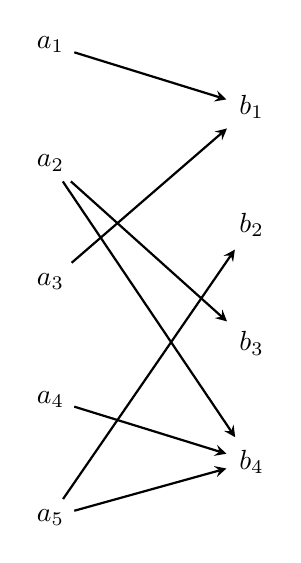
\begin{tikzpicture}[->,>=stealth,shorten >=1pt,auto,node distance=1.5cm,thick,main node/.style={scale=0.9,circle,draw,font=\sffamily\normalsize}]
            \node[] (1) {$a_1$};
            \node[] (2) [below of = 1] {$a_2$};
            \node[] (3) [below of = 2] {$a_3$};
            \node[] (4) [below of = 3] {$a_4$};
            \node[] (5) [below of = 4] {$a_5$};

            \node[] (a) [right of = 1, xshift = 30, yshift = -22.5] {$b_1$};
            \node[] (b) [below of = a] {$b_2$};
            \node[] (c) [below of = b] {$b_3$};
            \node[] (d) [below of = c] {$b_4$};

            \path[every node/.style={font=\sffamily\small}]
                (1) edge (a)
                (2) edge (c)
                (2) edge (d)
                (3) edge (a)
                (4) edge (d)
                (5) edge (b)
                (5) edge (d)
                ;
        \end{tikzpicture}
        \caption{Rappresentazione grafica della relazione $R$ sopra definita.}
    \end{figure}

    Il terzo metodo di rappresentazione, invece, prevede la refinizione di una matrice $M$ (o tabella) le cui righe e colonne sono indicizzate rispettivamente dall'insieme $A$ e dall'insieme $B$. Ogni entrata $m_{i,j}$ di tale matrice è un valore binario 0 o 1, dove $m_{i,j}$ è posta uguale ad 1 se $R(a_i, b_j)$, altrimenti è posta a 0.
    \[m_{i,j} = \soe{ll}{
        0 & \text{se } (a_i, b_j) \notin R \\
        1 & \text{se } (a_i, b_j) \in R
    }\] 
    
    \begin{figure}[H]
        \centering
        \begin{tabular}{c|cccc}
            & $b_1$ & $b_2$ & $b_3$ & $b_4$ \\
            \hline
            $a_1$ & 1 & 0 & 0 & 0 \\
            $a_2$ & 0 & 0 & 1 & 1 \\
            $a_3$ & 1 & 0 & 0 & 0 \\
            $a_4$ & 0 & 0 & 0 & 1 \\
            $a_5$ & 0 & 0 & 0 & 1 \\
        \end{tabular}
        \caption{Rappresentazione matriciale della relazione $R$ sopra definita.}
    \end{figure}
    
    Per relazioni binarie con molte coppie, tali due rappresentazioni risultano decisamente pià compatte. Quando una relazione binaria è definita su un singolo insieme, ossia $R \subseteq A \times A$, la sua rappresentazione grafica può essere ulteriormente compressa. Ad esempio, la relazione binaria $R' = \{(a_1, a_2), (a_1, a_3), (a_2, a_2), (a_3,a_5), (a_5, a_3)\}$ può essere rappresentata come segue.

    \begin{figure}[H]
        \centering
        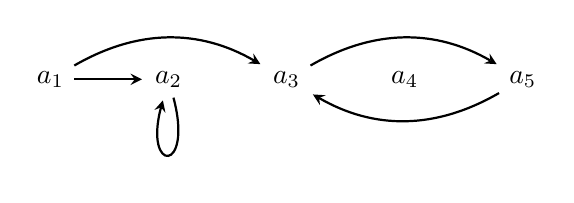
\begin{tikzpicture}[->,>=stealth,shorten >=1pt,auto,node distance=1.5cm,thick,main node/.style={scale=0.9,circle,draw,font=\sffamily\normalsize}]
            \node[] (1) {$a_1$};
            \node[rectangle, draw] (2) [draw = white, right of = 1] {$a_2$};
            \node[] (3) [right of = 2] {$a_3$};
            \node[] (4) [right of = 3] {$a_4$};
            \node[] (5) [right of = 4] {$a_5$};

            \path[every node/.style={font=\sffamily\small}]
                (1) edge (2)
                (1) edge [bend left] (3)
                (2) edge [loop below, distance = 1cm] (2)
                (3) edge [bend left] (5)
                (5) edge [bend left] (3)
                ;
        \end{tikzpicture}
        \caption{Rappresentazione grafica della relazione $R'$.}
    \end{figure}

    \section{Inversione e composizione di relazioni}

    Essendo le relazioni una generalizzazione delle funzioni (in particolare le relazioni binarie), risulta naturale estenedere i concetti di funzione inversa e composta anche al mondo delle relazioni. Per le funzioni abbiamo visto come se $f(x) = y$ allora $f^{-1}(y) = x$. Utilizzando la notazione di relazione per tali due funzioni, avremmo che $(x,y) \in f$ e che $(y,x) \in f^{-1}$. Risulta quindi evidente che l'inversione di una relazione non è altro che il suo \curlyquotes{specchiamento}. Ad esempio, l'inversa della relazione $R$ descrivente \curlyquotes{$x$ è padre di $y$} risulta essere la relazione $R^{-1}$ descrivente \curlyquotes{$y$ è figlio di $x$}.

    \begin{frameddefn}{Relazione inversa}
        Data la relazione $R \subseteq A \times B$, la relazione inversa di $R$ è definita come $R \subseteq B \times A$, dove:
        \[R^{-1} = \{(b,a) \in B \times A \mid (a,b) \in R\}\]
    \end{frameddefn}

    Osserviamo come, a differenza delle funzioni, per le relazioni esista \textit{sempre} la relazione inversa: nel caso delle funzioni il problema è dato dalla possibilità di ottenere un'inversa non funzionale (dunque una funzione mal posta), ma nelle relazioni generiche tale problema non sussiste.
    
    Ricavare l'inversa di una relazione risulta estremamente facile per definizione stessa: è sufficiente invertire l'ordine degli elementi all'interno di ogni tupla della relazione. Ad esempio, data la seguente relazione $R$:
    \[R = \{(a_1, b_1), (a_2, b_3), (a_2, b_4), (a_3, b_1), (a_4, b_4), (a_5, b_2), (a_5, b_5)\}\]

    l'inversa sarà data da:
    \[R^{-1} = \{(b_1, a_1), (b_3, a_2), (b_4, a_2), (b_1, a_3), (b_4, a_4), (b_2, a_5), (b_5, a_5)\}\]

    Nel caso delle relazioni binarie, ricavare l'inversa risulta ancor più facile tramite le sue due rappresentazioni alternative, ossia tramite grafo e tramite matrice. Nel primo caso, è sufficiente invertire la direzione di tutte le frecce, mentre nel secondo caso è sufficiente \textit{trasporre} la matrice, ossia invertire le sue righe con le sue colonne. 


    \begin{figure}[H]
        \centering
        \begin{tabular}{c c c}
            \begin{tabular}{c}
                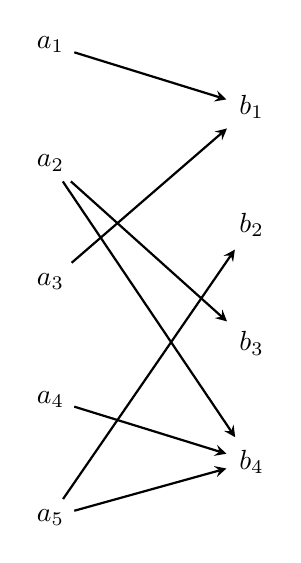
\begin{tikzpicture}[->,>=stealth,shorten >=1pt,auto,node distance=1.5cm,thick,main node/.style={scale=0.9,circle,draw,font=\sffamily\normalsize}]
                    \node[] (1) {$a_1$};
                    \node[] (2) [below of = 1] {$a_2$};
                    \node[] (3) [below of = 2] {$a_3$};
                    \node[] (4) [below of = 3] {$a_4$};
                    \node[] (5) [below of = 4] {$a_5$};

                    \node[] (a) [right of = 1, xshift = 30, yshift = -22.5] {$b_1$};
                    \node[] (b) [below of = a] {$b_2$};
                    \node[] (c) [below of = b] {$b_3$};
                    \node[] (d) [below of = c] {$b_4$};

                    \path[every node/.style={font=\sffamily\small}]
                        (1) edge (a)
                        (2) edge (c)
                        (2) edge (d)
                        (3) edge (a)
                        (4) edge (d)
                        (5) edge (b)
                        (5) edge (d)
                        ;
                \end{tikzpicture}
            \end{tabular}
            &\qquad\qquad\qquad& 

            \begin{tabular}{c}
                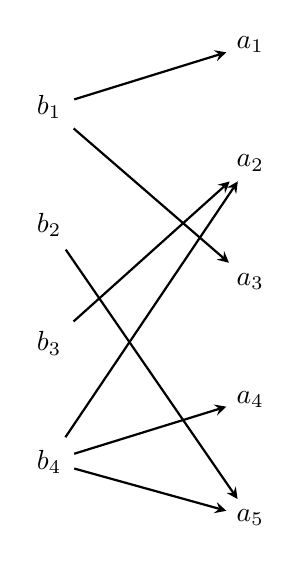
\begin{tikzpicture}[<-,>=stealth,shorten >=1pt,auto,node distance=1.5cm,thick,main node/.style={scale=0.9,circle,draw,font=\sffamily\normalsize}]
                    \node[] (1) {$a_1$};
                    \node[] (2) [below of = 1] {$a_2$};
                    \node[] (3) [below of = 2] {$a_3$};
                    \node[] (4) [below of = 3] {$a_4$};
                    \node[] (5) [below of = 4] {$a_5$};

                    \node[] (a) [left of = 1, xshift = -30, yshift = -22.5] {$b_1$};
                    \node[] (b) [below of = a] {$b_2$};
                    \node[] (c) [below of = b] {$b_3$};
                    \node[] (d) [below of = c] {$b_4$};

                    \path[every node/.style={font=\sffamily\small}]
                        (1) edge (a)
                        (2) edge (c)
                        (2) edge (d)
                        (3) edge (a)
                        (4) edge (d)
                        (5) edge (b)
                        (5) edge (d)
                        ;
                \end{tikzpicture}
            \end{tabular}

            \\

            \begin{tabular}{c|cccc}
                & $b_1$ & $b_2$ & $b_3$ & $b_4$ \\
                \hline
                $a_1$ & 1 & 0 & 0 & 0 \\
                $a_2$ & 0 & 0 & 1 & 1 \\
                $a_3$ & 1 & 0 & 0 & 0 \\
                $a_4$ & 0 & 0 & 0 & 1 \\
                $a_5$ & 0 & 0 & 0 & 1 \\
            \end{tabular}

            & &

            \begin{tabular}{c|ccccc}
                & $a_1$ & $a_2$ & $a_3$ & $a_4$ & $a_5$ \\
                \hline
                $b_1$ & 1 & 0 & 1 & 0 & 0 \\
                $b_2$ & 0 & 0 & 0 & 0 & 0 \\
                $b_3$ & 0 & 1 & 0 & 0 & 0 \\
                $b_4$ & 0 & 1 & 0 & 1 & 1 \\
            \end{tabular}
        \end{tabular}
        \caption{La relazione $R$ (sinistra) sopra definita e la sua inversa $R^{-1}$ (destra), rappresentate tramite grafi e matrici.}
    \end{figure}

    Passiamo ora alla composizione tra relazioni. Analogamente a prima, ricaviamo la generalizzazione passando tramite quello che abbiamo già detto per le funzioni. Siano $f : X \to Y$ e $g : A \to B$ due funzioni. Supponiamo che $f(x) = y$ e $g(y) = z$, implicando che $(g \circ f)(x) = z$. Utilizzando la notazione di relazione per tali due funzioni, dati $(x,y) \in f$ e $(y,z) \in g$ otteniamo che $(x,z) \in g \circ f$.

    Fino a qui, tutto risulta abbastanza intuitivo. Osserviamo inoltre come nelle funzioni affinchè sia possibile comporre $f$ con $g$ -- dunque ricavare $g \circ f$ -- è necessario che $f(X) \subseteq A$. Questa condizione necessaria viene estesa in modo naturale alle relazioni. In particolare, possiamo imporre direttamente che $Y = A$ invece di $f(X) = A$ poiché nelle relazioni è concessa l'assenza di alcuni elementi. 

    \begin{frameddefn}{Relazione composta}
        Date le relazioni binarie $R \subseteq A \times B$ e $S \subseteq B \times C$, la relazione composta tra $R$ e $S$ è definita come $S \circ R \subseteq A \times C$, dove:
        \[S \circ R = \{(a,c) \in A \times C \mid \exists b \in B \text{ tale che } R(a,b) \text{ e } S(b,c)\}\]
    \end{frameddefn}

    Consideriamo quindi le seguenti due relazioni $R$ ed $S$:
    \[R = \{(a,b), (b,b), (b,d), (c,a), (d,a)\} \qquad S = \{(a,d), (a,b), (b,c), (d,b)\}\]

    Per ricavare la composta $S \circ R$, consideriamo una alla volta ogni coppia $(x,y) \in R$ e cerchiamo tutte le coppie della forma $(y,z)$ che si trovino in $S$. Per ogni coppia trovata in $S$, aggiungiamo la coppia $(x,z)$ a $S \circ R$. 
    \begin{enumerate}
        \item Consideriamo $(a,b) \in R$. Poiché $(b,c) \in S$, aggiungiamo $(a,c)$ a $S \circ B$
        \item Consideriamo $(b,b) \in R$. Poiché $(b,c) \in S$, aggiungiamo $(b,c)$ a $S \circ B$
        \item Consideriamo $(b,d) \in R$. Poiché $(d,b) \in S$, aggiungiamo $(b,b)$ a $S \circ B$
        \item Consideriamo $(c,a) \in R$. Poiché $(a,d), (a,b) \in S$, aggiungiamo $(c,d)$ e $(c,b)$ a $S \circ B$
        \item Consideriamo $(d,a) \in R$. Poiché $(a,d), (a,b) \in S$, aggiungiamo $(d,d)$ e $(d,b)$ a $S \circ B$
    \end{enumerate}

    Una volta completato il processo, concludiamo che:
    \[S \circ R = \{(a,c), (b,b), (b,c), (c,b), (c,d), (d,b), (d,d)\}\]

    Ovviamente, è facile osservare che come per le funzioni l'ordine di composizione sia fondamentale. Ad esempio, in questo caso abbiamo che $S \circ R \neq R \circ S$ poiché:
    \[R \circ S = \{(a,a), (a,b), (a,d), (b,a), (d,b), (d,d)\}\] 

    Risulta evidente che calcolare una composizione tra relazioni sia estremamente laborioso nel caso in cui le relazioni $R$ ed $S$ involte contengano molti elementi (in particolare ci richiede di svolgere $\abs{R} \cdot \abs{S}$ controlli). Tuttavia, il processo risulta leggermente più veloce quando vengono utilizzate le due notazioni alternative, in particolare quella tramite grafi. In questa notazione, è sufficiente rappresentare le due relazioni $R \subseteq A \times B$ e $S \subseteq B \times C$ una accanto all'altra, utilizzando l'insieme $B$ come ponte tra di loro. Ogni freccia da $A$ a $B$ seguita da una freccia da $B$ a $C$ corrisponde ad una freccia da $A$ a $C$ che descrive la composizione.

    Ad esempio, consideriamo le due relazioni $R' \subseteq A \times B$ ed $S' \subseteq B \times C$ definite come:
    \[R' = \{(a_1, b_1), (a_1,b_2), (a_2, b_4), (a_3, b_1), (a_4, b_4), (a_5, b_2), (a_5, b_5)\}\]
    \[S' = \{(b_1,c_1), (b_1, c_2), (b_2, c_1), (b_2, c_4), (b_2, c_5), (b_3,c_6)\}\]

    Graficamente otteniamo la seguente rappresentazione.

    \begin{figure}[H]
        \centering
        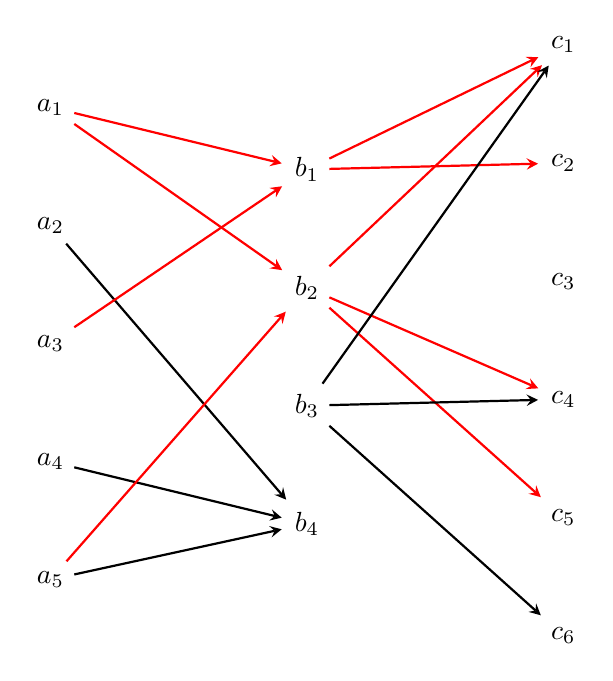
\begin{tikzpicture}[->,>=stealth,shorten >=1pt,auto,node distance=1.5cm,thick,main node/.style={scale=0.9,circle,draw,font=\sffamily\normalsize}]
            \node[] (1) {$a_1$};
            \node[] (2) [below of = 1] {$a_2$};
            \node[] (3) [below of = 2] {$a_3$};
            \node[] (4) [below of = 3] {$a_4$};
            \node[] (5) [below of = 4] {$a_5$};

            \node[] (a) [right of = 1, xshift = 50, yshift = -22.5] {$b_1$};
            \node[] (b) [below of = a] {$b_2$};
            \node[] (c) [below of = b] {$b_3$};
            \node[] (d) [below of = c] {$b_4$};

            \node[] (c1) [right of = a, xshift = 50, yshift = 45] {$c_1$};
            \node[] (c2) [below of = c1] {$c_2$};
            \node[] (c3) [below of = c2] {$c_3$};
            \node[] (c4) [below of = c3] {$c_4$};
            \node[] (c5) [below of = c4] {$c_5$};
            \node[] (c6) [below of = c5] {$c_6$};

            \path[every node/.style={font=\sffamily\small}]
                (1) edge[color=red] (a)
                (1) edge[color=red] (b)
                (2) edge (d)
                (3) edge[color=red] (a)
                (4) edge (d)
                (5) edge[color=red] (b)
                (5) edge (d)

                (a) edge[color=red] (c1)
                (a) edge[color=red] (c2)
                (b) edge[color=red] (c1)
                (b) edge[color=red] (c4)
                (b) edge[color=red] (c5)
                (c) edge (c1)
                (c) edge (c4)
                (c) edge (c6)
                ;
        \end{tikzpicture}
        \caption{Composizione tra due relazioni tramite grafi. Le frecce rosse dettano la composizione finale in quanto fungono da \curlyquotes{ponte} tra $A$ e $C$.}
    \end{figure}

    Seguendo le frecce rosse, otteniamo facilmente che la composizione $S \circ R$ sia:
    \[S' \circ R' = \{(a_1, c_1), (a_1,c_2), (a_1, c_4), (a_1,c_5), (a_3, c_1), (a_3, c_2),  (a_5, b_1), (a_5, c_4), (a_5, c_5)\}\]

    In particolare, osserviamo come sia possibile ottenere alcune tuple di $S' \circ R'$ in più di un modo. Ad esempio, la tupla $(a_1,c_1) \in S' \circ R'$ è data sia da $R'(a_1,b_1)$ e $S'(b_1, c_1)$ sia da $R(a_1, b_2)$ e $S'(b_2, c_1)$. Essendo $S' \circ R'$ un insieme, la composizione viene contata solo una volta.

    Per quanto riguarda la rappresentazione matriciale, invece, la composizione tra due relazioni è data dal \textit{prodotto matriciale} (con valore massimo 1) tra le due matrici che le rappresentano (vedere \href{https://it.wikipedia.org/wiki/Moltiplicazione_di_matrici}{questo link} per un ripasso sul prodotto matriciale). Ad esempio, consideriamo le due tabelle descriventi $R'$ ed $S'$ come definite sopra:

    \begin{figure}[H]
        \centering
        \begin{tabular}{c c c}
            \begin{tabular}{c|cccc}
                & $b_1$ & $b_2$ & $b_3$ & $b_4$ \\
                \hline
                $a_1$ & 1 & 1 & 0 & 0 \\
                $a_2$ & 0 & 0 & 0 & 1 \\
                $a_3$ & 1 & 0 & 0 & 0 \\
                $a_4$ & 0 & 0 & 0 & 1 \\
                $a_5$ & 0 & 1 & 0 & 1 \\
            \end{tabular}

            & &

            \begin{tabular}{c|cccccc}
                & $c_1$ & $c_2$ & $c_3$ & $c_4$ & $c_5$ & $c_6$ \\
                \hline
                $b_1$ & 1 & 1 & 0 & 0 & 0 & 0 \\
                $b_2$ & 1 & 0 & 0 & 1 & 1 & 0 \\
                $b_3$ & 1 & 0 & 0 & 1 & 0 & 1 \\
                $b_4$ & 0 & 0 & 0 & 0 & 0 & 0 \\
            \end{tabular}
        \end{tabular}
        \caption{Rappresentazione matriciale di $R'$ ed $S'$.}
    \end{figure}

    Il prodotto matriciale tra $M_{R'}$ e $M_{S'}$ corrisponde a:
    \[M_{R'} \cdot M_{S'} = \smat{
        1 & 1 & 0 & 0 \\
        0 & 0 & 0 & 1 \\
        1 & 0 & 0 & 0 \\
        0 & 0 & 0 & 1 \\
        0 & 1 & 0 & 1
    } \cdot \smat{
        1 & 1 & 0 & 0 & 0 & 0 \\
        1 & 0 & 0 & 1 & 1 & 0 \\
        1 & 0 & 0 & 1 & 0 & 1 \\
        0 & 0 & 0 & 0 & 0 & 0 \\
    } = \smat{
        2 & 1 & 0 & 1 & 1 & 0 \\
        0 & 0 & 0 & 0 & 0 & 0 \\
        1 & 1 & 0 & 0 & 0 & 0 \\
        0 & 0 & 0 & 0 & 0 & 0 \\
        1 & 0 & 0 & 1 & 1 & 0 \\
    }\]

    Definiamo ora l'operatore $\delta$ che presa una matrice in input restituisce una matrice equivalente a quella in input ma le cui entrate valgono massimo 1. La matrice $M_{S' \circ R'}$ della composizione $S' \circ R'$ corrisponde all'applicazione di tale funzione sul prodotto matriciale tra $M_{R'}$ e $M_{S'}$, ossia:
    \[M_{S' \circ R'} = \delta(M_{R'} \cdot M_{S'}) = \smat{
        1 & 1 & 0 & 1 & 1 & 0 \\
        0 & 0 & 0 & 0 & 0 & 0 \\
        1 & 1 & 0 & 0 & 0 & 0 \\
        0 & 0 & 0 & 0 & 0 & 0 \\
        1 & 0 & 0 & 1 & 1 & 0 \\
    }\]

    \section{Proprietà delle relazioni binarie}

    Nelle sezioni precedenti abbiamo accennato come le funzioni siano uno speciale tipo di relazione binaria. Relazioni che rispettano la proprietà di \textit{ben definizione} di una funzione, ossia la presenza di esattamente un output per ogni input, vengono dette \textbf{funzionali}. Quando una relazione è funzionale, è possibile utilizzare anche la notazione $R(a) = b$ in quanto $R$ è a tutti gli effetti una funzione.

    \begin{frameddefn}{Relazione funzionale}
        Data una relazione $R \subseteq A \times B$, diciamo che $R$ è una relazione funzionale se per ogni $a \in A$ esiste esattamente un elemento $b \in B$ tale che $R(a,b)$. 
    \end{frameddefn}

    Le relazioni binarie godono di molte caratteristiche comuni. In particolare, ci concentreremo su relazioni binarie definite su un unico insieme, ossia $R \subseteq A \times A$.
    
    Consideriamo le relazioni \curlyquotes{$n$ è minore di $m$} e \curlyquotes{$n$ è al massimo $m$} definite sui numeri naturali, ossia le relazioni $< \subseteq \N \times \N$ e $\leq \subseteq \N \times \N$. Osserviamo come per ogni numero $n \in \N$ valga che $n \leq n$ (ossia $(n,n) \in \leq$). Quando ciò accade per ogni elemento, diciamo che la relazione è \textbf{riflessiva}. Per la relazione $<$, invece, per ogni numero $n \in \N$ vale che $n \not < n$ (ossia $(n,n) \notin <$). In questo caso diciamo che la relazione è \textbf{irriflessiva}.

    \begin{frameddefn}{Relazione riflessiva e irriflessiva}
        Data una relazione $R \subseteq A \times A$, diciamo che $R$ è:
        \begin{itemize}
            \item riflessiva se $\forall a \in A$ vale che $(a,a) \in R$
            \item irriflessiva se $\forall a \in A$ vale che $R(a,a) \notin R$
        \end{itemize}
    \end{frameddefn}

    Rimarchiamo che, a livello logico, affinché una relazione non sia riflessiva è sufficiente e necessario che vi sia almeno un elemento $a \in A$ per cui $(a,a) \notin R$.Analogamente, affinché una relazione non sia irriflessiva è sufficiente e necessario che vi sia almeno un elemento $a \in A$ per cui $(a,a) \in R$.
    \[R \subseteq A \times A \text{ non riflessiva} \iff \exists a \in A \text{ tale che } (a,a) \notin R\]
    \[R \subseteq A \times A \text{ non irriflessiva} \iff \exists a \in A \text{ tale che } (a,a) \in R\]
    
    Da questa osservazione deduciamo quindi che possano esserci relazioni che non sono nè riflessive nè irriflessive. Ad esempio, la relazione \curlyquotes{$x$ ha inviato un'email ad $y$} non è né riflessiva né irriflessiva: è possibile che qualcuno abbia inviato un'email a se stesso così come è possibile che qualcuno non l'abbia fatto.

    Consideriamo ora la relazione $R$ rappresentante \curlyquotes{$x$ è fratello di $y$}. Osserviamo come in modo naturale si abbia che se Mario è fratello di Luigi allora anche Luigi è fratello di Mario, ossia che se $R(x,y)$ allora deve anche valere che $R(y,x)$. Quando ciò accade per ogni coppia $(x,y) \in R$, la relazione viene detta \textbf{simmetrica}.

    \begin{frameddefn}{Relazione simmetrica}
        Data una relazione $R \subseteq A \times A$, diciamo che $R$ è simmetrica se per ogni coppia $x,y \in A$ ogni volta che si ha $R(x,y)$ si ha anche $R(y,x)$.
        \[\forall x,y \in A \text{ se } R(x,y) \text{ allora } R(y,x)\]
    \end{frameddefn}

    A livello logico, affinché una relazione non sia simmetrica è sufficiente e necessario che vi sia almeno una coppia $x,y \in A$ per cui si ha $R(x,y)$ ma non $R(y,x)$.
    \[R \subseteq A \times A \text{ non simmetrica} \iff \exists x,y \in A \text{ tali che } (x,y) \in R \text{ e } (y,x) \notin R\]

    Osserviamo quindi che in alcuni casi la simmetria possa essere soddisfata \curlyquotes{a vuoto}, ossia non vi sono coppie su cui verificare la validità della condizione. Questo è il caso della relazione vuota $R = \varnothing$: poiché non esistono coppie $(x,y)$ per cui $(x,y) \in \varnothing$, è sempre vero che quando la premessa $(x,y) \in \varnothing$ è vera anche la conseguenza $(y,x) \in \varnothing$ è vera (poiché la premessa è sempre falsa!). 

    Un esempio esplicito di relazione non simmetrica è dato dalla relazione $\leq$ vista precedentemente: prendendo qualsiasi coppia di numeri diversi, ad esempio $5$ e $3$, abbiamo che $3 \leq 5$ e $5 \not \leq 3$. Tuttavia, osserviamo che esistono effettivamente alcune coppie di numeri per cui \curlyquotes{vale la simmetria}. Difatti, per ogni numero $n \in \N$ abbiamo chiaramente che $n \leq n$ e che $n \leq n$! Ma questo già lo sapevamo in quanto $\leq$ è riflessiva\dots
    
    Di maggior interesse è invece considerare la proprietà \curlyquotes{opposta}, ossia il fatto che per ogni coppia di numeri $n,m \in \N$ si abbia che $n \leq m$ e $m \leq n$ solo quando $n = m$. In altre parole, non esistono due numeri distinti che siano simmetrici secondo $\leq$. Quando ciò si verifica, la relazione viene detta \textbf{anti-simmetrica}, nome che richiama il fatto che la simmetria si verifichi solo quando gli elementi coinvolti sono in realtà identici.

    \begin{frameddefn}{Relazione anti-simmetrica}
        Data una relazione $R \subseteq A \times A$, diciamo che $R$ è anti-simmetrica se per ogni coppia $x,y \in A$ ogni volta che si ha sia $R(x,y)$ sia $R(y,x)$ vale necessariamente che $x = y$.
        \[\forall x,y \in A \text{ se } R(x,y) \text{ e } R(y,x) \text{ allora } x = y\] 
    \end{frameddefn}

    A livello logico, affinché una relazione non sia anti-simmetrica è sufficiente e necessario che vi sia almeno una coppia $x,y \in A$ per cui si ha sia $R(x,y)$ sia $R(y,x)$ ma non $x = y$.
    \[R \subseteq A \times A \text{ non anti-simmetrica} \iff \exists x,y \in A \text{ tali che } R(x,y) \text{ e } R(y,x) \text{ ma } x \neq y\]

    Come nel caso della riflessività e della irriflessività, possono esserci relazioni che non sono né simmetriche né anti-simmetriche. Ad esempio, la seguente relazione $R \subseteq A \times A$ definita come:
    \[R = \{(a,b), (a,c), (c,a)\}\]
    non è simmetrica in quanto non esiste la coppia $(b,a)$ e neanché anti-simmetrica in quanto ci sono le coppie $(a,c), (c,a)$ ma $a \neq c$. Osserviamo anche come esistono relazioni che sono sia simmetriche sia anti-simmetriche. Ancora una volta, questo è il caso della relazione vuota $R = \varnothing$ poiché anche l'anti-simmetria è vera a vuoto!

    Prendiamo ancora in considerazione la relazione $leq$. Essa gode di un'ulteriore fondamentale proprietà utilizzata sempre in matematica: se ci sono tre elementi $a,b,c \in \N$ tali che $a \leq b$ e $b \leq c$, è sempre garantito che $a \leq c$ sia anche vero! Quando ciò si verifica, la relazione è detta \textbf{transitiva}.


    \begin{frameddefn}{Relazione transitiva}
        Data una relazione $R \subseteq A \times A$, diciamo che $R$ è transitiva se per ogni tripla $x,y,z \in A$ ogni volta che si ha sia $R(x,y)$ sia $R(y,z)$ vale necessariamente che $R(x,z)$.
        \[\forall x,y,z \in A \text{ se } R(x,y) \text{ e } R(y,z) \text{ allora } R(x,z)\] 
    \end{frameddefn}

    A livello logico, affinché una relazione non sia transitiva è sufficiente e necessario che vi sia almeno una tripla $x,y,z \in A$ per cui si ha sia $R(x,y)$ sia $R(y,z)$ ma non $R(x,z)$.
    \[R \subseteq A \times A \text{ non transitiva} \iff \exists x,y,z \in A \text{ tali che } R(x,y) \text{ e } R(y,z) \text{ ma non } R(x,z)\]

    La relazione \curlyquotes{$x$ è padre di $y$} è l'esempio più immediato di relazione non transitiva: se Aldo è padre di Giovanni e Giovanni è padre di Giacomo, non è vero che Aldo è padre di Giacomo.

    \section{Chiusura transitiva}

    Consideriamo la relazione $R = \{(a,b), (a,d), (b,c), (c,e)\}$ definita sull'insieme $A = \{a,b,c,d,e\}$. Notiamo facilmente come tale relazione non sia transitiva in quanto esistono le coppie $(a,b), (b,c)$ e le coppie $(b,c), (c,e)$ ma non la coppie $(a,c)$ e $(b,e)$.

    \begin{figure}[H]
        \centering
        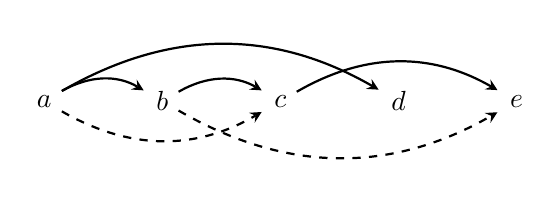
\begin{tikzpicture}[->,>=stealth,shorten >=1pt,auto,node distance=1.5cm,thick,main node/.style={scale=0.9,circle,draw,font=\sffamily\normalsize}]
            \node[] (1) {$a$};
            \node[] (2) [right of = 1] {$b$};
            \node[] (3) [right of = 2] {$c$};
            \node[] (4) [right of = 3] {$d$};
            \node[] (5) [right of = 4] {$e$};

            \path[every node/.style={font=\sffamily\small}]
                (1) edge [bend left] (2)
                (1) edge [bend left] (4)
                (2) edge [bend left] (3)
                (3) edge [bend left] (5)
                (1) edge [bend right, dashed] (3)
                (2) edge [bend right, dashed] (5)
                ;
        \end{tikzpicture}
        \caption{La relazione $R$ in esempio. Le frecce tratteggiate indicano le coppie mancanti.}
        \label{chius_trans_1}
    \end{figure}
    
    Consideriamo ora la relazione $R'$ ottenuta aggiungendo ad $R$ le due coppie $(a,c)$ e $(b,e)$, ossia $R' = R \cup \{(a,c), (b,e)\}$. Aggiungendo tali coppie, abbiamo risolto il problema inerente alle coppie $(a,b), (b,c)$ e le coppie $(b,c), (c,e)$, rendendo la transitività valida per loro. Tuttavia, questa aggiunta non ha completamente risolto il problema: abbiamo introdotto nuove coppie la cui rompe ancora la transitività. In particolare, osserviamo che l'aggiunta della coppia $(a,c)$ implichi che ora in $R'$ vi siano le coppie $(a,c), (c,e)$ ma non la coppia $(a,e)$. Similmente, l'aggiunta della coppia $(b,e)$ implica che vi siano le coppie $(a,b), (b,e)$, ma non la coppia $(a,e)$.

    \begin{figure}[H]
        \centering
        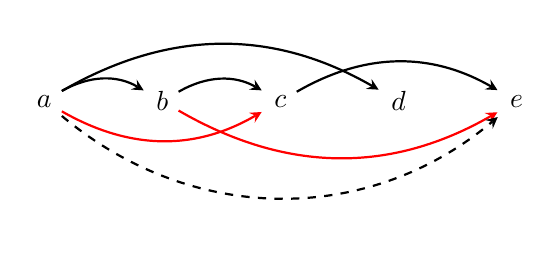
\begin{tikzpicture}[->,>=stealth,shorten >=1pt,auto,node distance=1.5cm,thick,main node/.style={scale=0.9,circle,draw,font=\sffamily\normalsize}]
            \node[] (1) {$a$};
            \node[] (2) [right of = 1] {$b$};
            \node[] (3) [right of = 2] {$c$};
            \node[] (4) [right of = 3] {$d$};
            \node[] (5) [right of = 4] {$e$};

            \path[every node/.style={font=\sffamily\small}]
                (1) edge [bend left] (2)
                (1) edge [bend left] (4)
                (2) edge [bend left] (3)
                (3) edge [bend left] (5)
                (1) edge [bend right, color = red] (3)
                (2) edge [bend right, color = red] (5)
                (1) edge [bend right = 40, dashed] (5)
                ;
        \end{tikzpicture}
        \caption{Le frecce rosse rappresentano le coppie in $R'$ aggiunte ad $R$. Le frecce tratteggiate indicano le coppie mancanti in $R'$.}
    \end{figure}

    Consideriamo quindi la relazione $R''$ ottenuta aggiungendo ad $R'$ la coppia $(a,e)$, ossia $R'' = R' \cup \{(a,e)\}$. Osserviamo come questa volta la transitività sia effettivamente soddisfatta, dunque $R''$ è una relazione che \textit{estende} $R$ e soddisfa la transitività. In particolare, $R''$ è anche la \textit{più piccola} relazione con tali proprietà. Questa tipologia di estensione viene detta \textbf{chiusura transitiva} di $R$.

    \begin{figure}[H]
        \centering
        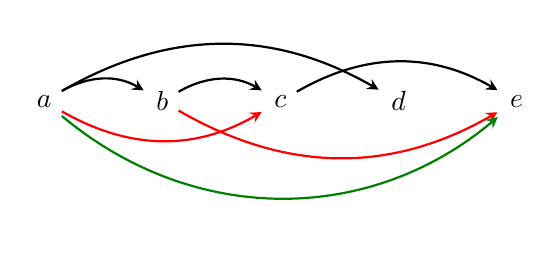
\begin{tikzpicture}[->,>=stealth,shorten >=1pt,auto,node distance=1.5cm,thick,main node/.style={scale=0.9,circle,draw,font=\sffamily\normalsize}]
            \node[] (1) {$a$};
            \node[] (2) [right of = 1] {$b$};
            \node[] (3) [right of = 2] {$c$};
            \node[] (4) [right of = 3] {$d$};
            \node[] (5) [right of = 4] {$e$};

            \path[every node/.style={font=\sffamily\small}]
                (1) edge [bend left] (2)
                (1) edge [bend left] (4)
                (2) edge [bend left] (3)
                (3) edge [bend left] (5)
                (1) edge [bend right, color = red] (3)
                (2) edge [bend right, color = red] (5)
                (1) edge [bend right = 40, color = Green] (5)
                ;
        \end{tikzpicture}
        \caption{La freccia verde rappresenta la coppia in $R''$ aggiunta ad $R'$.}
        \label{chius_trans_2}
    \end{figure}

    \begin{frameddefn}{Chiusura transitiva.}
        Data una relazione $R \subseteq A \times A$, definiamo la chiusura transitiva di $R$, indicata con $R^+$, come la più piccola relazione transitiva che estende $R$, ossia tale che:
        \begin{itemize}
            \item $R \subseteq R^+$
            \item $R^+$ è transitiva
            \item Per ogni relazione transitiva $S$ tale che $R \subseteq S$ vale anche che $R^+ \subseteq S$
        \end{itemize}
    \end{frameddefn}

    Il concetto di chiusura transitiva gioca un ruolo fondamentale in matematica, permettendo di modellare molte realtà. Supponiamo ad esempio di avere un insieme di città $C = \{c_1, \ldots, c_n\}$ e supponiamo che la relazione $S$ descriva l'esistenza di una strada tra due città, ossia $R(c_i, c_j)$ se e solo se esiste una strada da $c_i$ a $c_j$. È facile osservare come la chiusura transitiva $S^+$ consista nella relazione descrivente la possibilità di arrivare da una città all'altra, ossia $S^+(c_i, c_j)$ se e solo se è possibile andare da $c_i$ a $c_j$ tramite una serie di strade.

    Consideriamo ancora la relazione $R$ dell'esempio precedente (\Cref{chius_trans_1}). Notiamo come la stessa idea di percorribilità della serie di strade possa essere applicato anche alla relazione $R$: \curlyquotes{percorrendo} la coppia $(a,b)$ poi la coppia $(b,c)$ otteniamo che sia possibile andare da $a$ a $c$. Generalizziamo quindi tale idea con il concetto di \textbf{relazione di raggiungibilità}.

    \begin{frameddefn}{Relazione di raggiungibilità}
        Sia $R \subseteq A \times A$ una relazione. Dati due elementi $a,b \in A$, definiamo un cammino su $R$ da $a$ a $b$ come una sequenza finita di elementi $x_1, \ldots, x_k \in A$ tali che:
        \[R(a, x_1), R(x_1, x_2), \ldots, R(x_{k-1}, x_k), R(x_k, b)\]

        Definiamo la relazione di raggiungibilità su $R$, indicata con $R^c$, come la relazione data da tutte le coppie di $A$ per cui esiste un cammino su $R$:
        \[R^c = \{(a,b) \mid \text{Esiste un cammino da $a$ a $b$ su $R$}\}\]
    \end{frameddefn}

    Una volta intuita l'idea dietro il concetto di raggiungibilità, risulta facile osservare come il concetto di relazione di raggiungibilità e di chiusura transitiva siano del tutto equivalenti, ossia che $R^+ = R^c$ per ogni relazione $R$: percorrendo due cammini dove la fine del primo coincide con l'inizio del secondo otteniamo un nuovo cammino che estende $R$.

    \begin{framedthm}{Chiusura transitiva (2° def.)}
        Sia $R \subseteq A \times A$ una relazione. Allora, vale che $R^+ = R^c$
    \end{framedthm}

    \begin{proof}
        Omessa.
    \end{proof}

    Ma se i due concetti sono equivalenti, perchè definirli entrambi? La risposta è nel \textit{cambio di prospettiva} rispetto ai due concetti. L'idea di raggiungibilità ci fornisce un modo pratico per computare facilmente la chiusura transitiva di una relazione. Difatti, utilizzando il concetto di raggiungibilità e la rappresentazione grafica di una relazione risulta immediato calcolarne la chiusura transitiva: se ci sono due cammini che ne formano uno più lungo, aggiungiamo il nuovo cammino e ricontrolliamo l'esistenza di altri cammini ottenibili, finché non ve ne saranno più.

    Questo ci permette quindi di ridurre leggermente la complessità della procedura, ma non di molto: trovare tutti cammini ottenibili nel caso di relazioni con molte coppie potrebbe richiedere parecchio tempo. Esiste quindi una procedura più \curlyquotes{meccanica} per calcolare una chiusura transitiva? Fortunatamente, la risposta è sì!

    Facciamo prima un passo indietro. Abbiamo detto che il concetto di cammino corrisponde all'esistenza di una successione di coppie che ci permettono di raggiungere l'elemento finale del cammino partendo da un elemento iniziale. Riprendiamo ancora una volta la relazione $R$ dell'esempio precedente (\Cref{chius_trans_1}). Cambiamo leggermente la rappresentazione di $R$, utilizzando la rappresentazione a doppio insieme.
    
    Per ogni $i \in \N$, indichiamo con $R^i$ l'insieme dei cammini su $R$ aventi lunghezza 1, ossia formati da una singola coppia. Per definizione stessa abbiamo che $R^1 = R$.

    \begin{figure}[H]
        \centering
        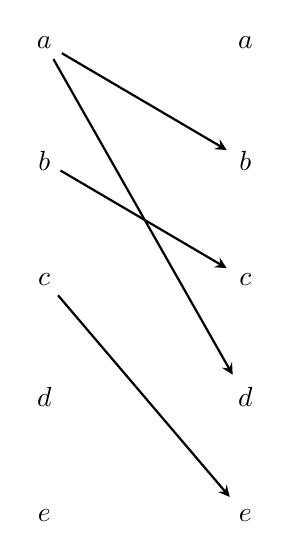
\begin{tikzpicture}[->,>=stealth,shorten >=1pt,auto,node distance=1.5cm,thick,main node/.style={scale=0.9,circle,draw,font=\sffamily\normalsize}]
            \node[] (1) {$a$};
            \node[] (2) [below of = 1] {$b$};
            \node[] (3) [below of = 2] {$c$};
            \node[] (4) [below of = 3] {$d$};
            \node[] (5) [below of = 4] {$e$};

            \node[] (a) [right of = 1, xshift = 30] {$a$};
            \node[] (b) [below of = a] {$b$};
            \node[] (c) [below of = b] {$c$};
            \node[] (d) [below of = c] {$d$};
            \node[] (e) [below of = d] {$e$};

            \path[every node/.style={font=\sffamily\small}]
                (1) edge (b)
                (1) edge (d)
                (2) edge (c)
                (3) edge (e)
                ;
        \end{tikzpicture}
        \caption{Rappresentazione a doppio insieme di $R^1 = R$.}
    \end{figure}

    È facile notare come componendo $R$ con se stessa otteniamo tutti i cammini di lunghezza 2 definiti su $R$, ossia il cammino da $a$ a $c$ formato da $(a,b), (b,c)$ e il cammino da $b$ ad $e$ formato da $(b,c), (c,e)$. Otteniamo quindi che $R^2 = R \circ R$.

    \begin{figure}[H]
        \centering
        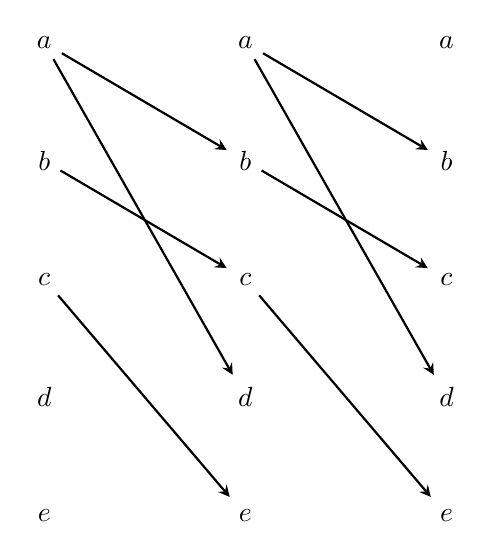
\begin{tikzpicture}[->,>=stealth,shorten >=1pt,auto,node distance=1.5cm,thick,main node/.style={scale=0.9,circle,draw,font=\sffamily\normalsize}]
            \node[] (1) {$a$};
            \node[] (2) [below of = 1] {$b$};
            \node[] (3) [below of = 2] {$c$};
            \node[] (4) [below of = 3] {$d$};
            \node[] (5) [below of = 4] {$e$};

            \node[] (a) [right of = 1, xshift = 30] {$a$};
            \node[] (b) [below of = a] {$b$};
            \node[] (c) [below of = b] {$c$};
            \node[] (d) [below of = c] {$d$};
            \node[] (e) [below of = d] {$e$};

            \node[] (xa) [right of = a, xshift = 30] {$a$};
            \node[] (xb) [below of = xa] {$b$};
            \node[] (xc) [below of = xb] {$c$};
            \node[] (xd) [below of = xc] {$d$};
            \node[] (xe) [below of = xd] {$e$};

            \path[every node/.style={font=\sffamily\small}]
                (1) edge (b)
                (1) edge (d)
                (2) edge (c)
                (3) edge (e)

                (a) edge (xb)
                (a) edge (xd)
                (b) edge (xc)
                (c) edge (xe)
                ;
        \end{tikzpicture}
        \caption{La composizione $R^2 = R \circ R = \{(a,c), (b,e)\}$.}
    \end{figure}
    
    Intuitivamente, componendo $R^2$ ancora una volta con $R$, otteniamo i cammini di lunghezza $3$ definiti su $R$.

    \begin{figure}[H]
        \centering
        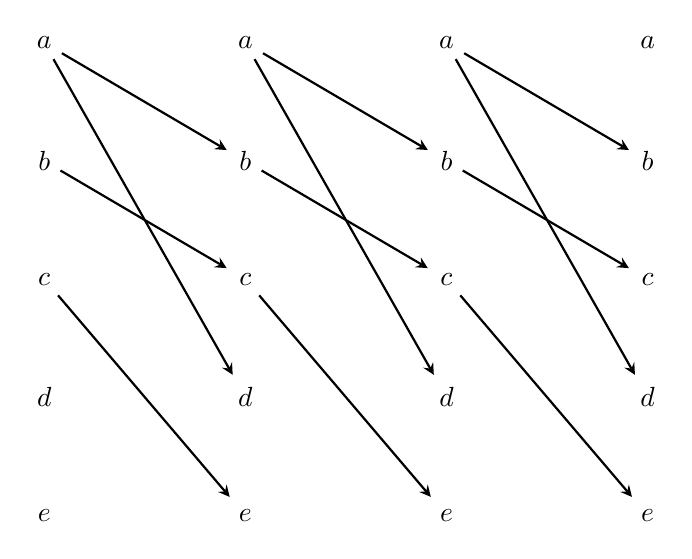
\begin{tikzpicture}[->,>=stealth,shorten >=1pt,auto,node distance=1.5cm,thick,main node/.style={scale=0.9,circle,draw,font=\sffamily\normalsize}]
            \node[] (1) {$a$};
            \node[] (2) [below of = 1] {$b$};
            \node[] (3) [below of = 2] {$c$};
            \node[] (4) [below of = 3] {$d$};
            \node[] (5) [below of = 4] {$e$};

            \node[] (a) [right of = 1, xshift = 30] {$a$};
            \node[] (b) [below of = a] {$b$};
            \node[] (c) [below of = b] {$c$};
            \node[] (d) [below of = c] {$d$};
            \node[] (e) [below of = d] {$e$};

            \node[] (xa) [right of = a, xshift = 30] {$a$};
            \node[] (xb) [below of = xa] {$b$};
            \node[] (xc) [below of = xb] {$c$};
            \node[] (xd) [below of = xc] {$d$};
            \node[] (xe) [below of = xd] {$e$};

            \node[] (ya) [right of = xa, xshift = 30] {$a$};
            \node[] (yb) [below of = ya] {$b$};
            \node[] (yc) [below of = yb] {$c$};
            \node[] (yd) [below of = yc] {$d$};
            \node[] (ye) [below of = yd] {$e$};

            \path[every node/.style={font=\sffamily\small}]
                (1) edge (b)
                (1) edge (d)
                (2) edge (c)
                (3) edge (e)

                (a) edge (xb)
                (a) edge (xd)
                (b) edge (xc)
                (c) edge (xe)

                (xa) edge (yb)
                (xa) edge (yd)
                (xb) edge (yc)
                (xc) edge (ye)
                ;
        \end{tikzpicture}
        \caption{La composizione $R^3 = R \circ R \circ R = \{(a,e)\}$.}
    \end{figure}

    Procedendo analogamente, ossia componendo $R^3$ con $R$, osserviamo come la relazione $R \circ R \circ R \circ R$ non contenga nessuna coppia. Difatti, non esistono cammini di lunghezza 4 definiti su $R$. Di conseguenza, possiamo essere certi che non esistano neanche cammini di lunghezza $5, 6, 7, \ldots$, concludendo che:
    \[R^c = R_1 \cup R_2 \cup R_3 = R \cup R \circ R \cup R \circ \R \circ R\]
    
    In generale, data una relazione $R$ è possibile calcolare $R^c$, e dunque anche $R^+$ per il teorema precedente, prendendo l'\textbf{unione infinita} di tutte le auto-composizioni di $R$.

    \begin{framedthm}{Chiusura transitiva (3° def.)}
        Sia $R \subseteq A \times A$. Allora, vale che:
        \[R^c = \bigcup_{i \in \N} R^i\]
        dove $R^i = \underbrace{R \circ \ldots \circ R}_{i \text{ volte}}$
    \end{framedthm}

    Sebbene l'unione è infinita, la sua computazione è in realtà \textbf{finita}: data la lunghezza massima $\ell$ di un cammino su $R$, sappiamo che per ogni $i > \ell$ l'insieme $R^i$ sarà sempre vuoto, dunque possiamo terminare la computazione direttamente a $R^\ell$. Per tanto, data una generica relazione $R$ possiamo calcolare $R^+$ componendo $R$ con se stessa finché otteniamo almeno un cammino di una lunghezza superiore alle precedenti, per poi prendere tutte le coppie ottenute nel mentre.

    \section{Relazioni d'equivalenza}

    Nelle precedenti sezioni abbiamo visto le principali proprietà che una relazione può assumere. Consideriamo ora la relazione di ugualianza $=$ sui numeri naturali, ossia:
    \[= \; \stackrel{def}{=}\; \{(n,m) \in \N \times \N \mid n \text{ è uguale a } m\}\]

    \textit{Nota:} il simbolo $\stackrel{def}{=}$ viene utilizzato per distinguere la relazione $=$ dal normale simbolo di ugualianza.

    È facile osservare come tale relazione rispetti tre delle proprietà principali:
    \begin{itemize}
        \item \textit{Riflessività}: per ogni $n \in \N$ abbiamo $n = n$
        \item \textit{Simmetria}: per ogni $n,m \in \N$ se $n = m$ allora $m = n$
        \item \textit{Transitività}: per ogni $n,m,k \in \N$, se $n = m$ e $m = k$ allora $n = k$
    \end{itemize}

    Una relazione che soddisfa queste tre proprietà viene detta \textbf{relazione d'equivalenza}, solitamente indicata con il simbolo $\sim$.

    \begin{frameddefn}{Relazione d'equivalenza}
        Data una relazione $\sim \subseteq A \times A$, diciamo che $\sim$ è una relazione d'equivalenza se è riflessiva, simmetrica e transitiva
    \end{frameddefn}

    Chiaramente, il concetto di ugualianza implica il concetto d'equivalenza, rendendo l'esempio precedente poco utile. Supponiamo ora di avere un insieme di $n$ macchine $M = \{m_1, \ldots, m_n\}$. Ognuna di tali macchine possiede un colore, scelto tra rosso, verde e blu. Consideriamo ora la relazione $R$ tale che $R(m_i, m_j)$ se e solo se $m_i$ è dello stesso colore di $m_j$. Osserviamo come anche $R$ soddisfi la riflessività, la simmetria e la transitività. Difatti, poiché in $R$ ci interessa solo ed esclusivamente il colore delle macchine, potremmo dire che $R$ definisce un concetto di \textit{equivalenza} tra le macchine in base al loro colore.

    In particolare, quindi, la relazione $R$ ci permette di \curlyquotes{raggruppare} le macchine in $M$ in base al loro colore. Ad esempio, data una macchina $m_i \in M$, se $m$ è rossa allora quest'ultima sarà in relazione solo ed esclusivamente con tutte le macchine rosse in $M$. L'insieme di elementi in relazione con $m_i$ è detto \textbf{classe d'equivalenza} su $R$.

    \begin{frameddefn}{Classe d'equivalenza}
        Sia $\sim \subseteq A \times A$ una relazione d'equivalenza. Dato un elemento $a \in A$, definiamo la sua classe d'equivalenza su $\sim$, indicata con $[a]_\sim$, come l'insieme di tutti gli elementi di $A$ in relazione con $a$ tramite $\sim$:
        \[[a]_\sim = \{ b \in A \mid a \sim b\}\]

        \textit{Nota}: quando il contesto lo rende chiaro, scriveremo direttamente $[a]$ invece di $[a]_\sim$.
    \end{frameddefn}

    Osserviamo come se due macchine $m_i$ e $m_j$ hanno lo stesso colore allora avremo che $[m_i] = [m_j]$ poiché entrambi gli insiemi conterranno le stesse identiche macchine. Se invece due macchine $m_i$ e $m_j$ possiedono colore diverso, avremo necessariamente che $[m_i] \cap [m_j] = \varnothing$ poiché entrambi gli insiemi conterranno macchine completamente diverse: se condividessero anche solo una macchina $m_k$, tutti gli elementi di $[m_i]$ e $[m_j]$ dovrebbero avere lo stesso colore di $m_k$, dunque $m_i$ ed $m_j$ avrebbero lo stesso colore!
    
    \begin{framedprop}{}
        Sia $\sim \subseteq A \times A$ una relazione d'equivalenza. Dati due elementi $a,b \in A$ si ha che:
        \begin{itemize}
        \item $a \sim b$ se e solo se $[a] = [b]$
        \item $a \not\sim b$ se e solo se $[a] \cap [b] = \varnothing$
        \end{itemize}
    \end{framedprop}

    Da queste due proprietà, risulta evidente come \underline{ogni} relazione d'equivalenza produca una \textit{partizione} dell'insieme su cui è definita. In particolare, la partizione sarà data dall'insieme di tutte le classi d'equivalenza definite su $A$ tramite $\sim$, detto \textbf{insieme quoziente}.
    
    \begin{frameddefn}{Insieme quoziente}
        Sia $\sim \subseteq A \times A$ una relazione d'equivalenza. Definiamo l'insieme quoziente di $A$ su $\sim$, indicato con $A/\sim$, come l'insieme di tutte le classi d'equivalenza indotte da $\sim$ su $A$:
        \[ A/\sim := \{ [a] \mid a \in A\}\]

        \textit{Nota:} $A/\sim$ è letto \curlyquotes{$A$ modulo $\sim$}
    \end{frameddefn}

    \begin{framedprop}{}
        Sia $\sim \subseteq A \times A$ una relazione d'equivalenza. L'insieme $A/\sim$ è una partizione di $A$.
    \end{framedprop}

    Nell'esempio precedente, l'insieme quoziente corrisponde a $M/\sim = \{[r], [v], [b]\}$, dove $r$ è una qualsiasi delle macchine rosse e lo stesso vale per $v$ e $b$ rispettivamente per le macchine verdi e blu.

    Vediamo ora un altro esempio di applicazione delle relazioni d'equivalenza. Sia $S \subseteq \N \times \N$ la relazione tale che $S(n,r)$ se e solo se $n = 5k+r$ per qualche $k \in \Z$. Con un po' di lavoro algebrico, ci convinciamo che tale relazione sia d'equivalenza (si provi a dimostrarlo per esercizio). In particolare, osserviamo come:
    \begin{itemize}
        \item $[0] = \{0, 5, 10, 15, \ldots\}$ poiché ognuno di essi può essere scritto come $5k+0$ per qualche $k \in \N$
        \item $[1] = \{1, 6, 11, 16, \ldots\}$ poiché ognuno di essi può essere scritto come $5k+1$ per qualche $k \in \N$
        \item $[2] = \{2, 7, 12, 17, \ldots\}$ poiché ognuno di essi può essere scritto come $5k+2$ per qualche $k \in \N$
        \item $[3] = \{3, 9, 13, 18, \ldots\}$ poiché ognuno di essi può essere scritto come $5k+3$ per qualche $k \in \N$
        \item $[4] = \{4, 0, 14, 19, \ldots\}$ poiché ognuno di essi può essere scritto come $5k+4$ per qualche $k$
    \end{itemize}

    In altre parole, ogni classe d'equivalenza $[r] \in \N/S$ corrisponde all'insieme dei numeri naturali che danno resto $r$ quando divisi per $5$. Questo concetto è alla base dell'\textit{algebra modulare}, la quale è di fondamentale importanza nell'informatica, soprattutto in ambiti come la crittografia.

    \section{Relazioni d'ordine}

    Nella sezione precedente abbiamo visto come le relazioni d'equivalenza, ossia relazioni riflessive, simmetriche e transitive, siano un potente modello matematico per descrivere l'\textit{equivalenza} tra elementi rispetto a qualche proprietà. In molte situazioni è necessario invece un modello che vada a caratterizzare il concetto di \textit{ordinamento} tra elementi. Esempio tipico di ciò è la relazione di minore uguale $\leq$ sui naturali, ossia:
    \[\leq \;\stackrel{def}{=}\; \{(n,m \in \N \times \N \mid n \text{ è minore uguale a } m)\}\]

    Abbiamo già discusso come tale relazione sia riflessiva e transitiva, ma non di equivaelenza in quanto non simmetrica. Bensì, tale relazione è anti-simmetrica, esprimendo come se due elementi siano comparabili vicendevolmente allora essi devono necessariamente essere lo stesso elemento. Una relazione riflessiva, anti-simmetrica e transitiva viene quindi detta \textbf{relazione d'ordine}, solitamente indicata col simbolo $\preceq$.

    \begin{frameddefn}{Relazione d'ordine}
        Data una relazione $\preceq \, \subseteq A \times A$, diciamo che $R$ è una relazione d'orinde se è riflessiva, anti-simmetrica e transitiva
    \end{frameddefn}

    Sorprendentemente, molte delle relazioni quotidiamente utilizzate in matematica sono d'ordine. Ad esempio, dato un insieme $X$, consideriamo la relazione di sottoinsieme su $\mathcal{P}(X)$, ossia:
    \[\subseteq \;\stackrel{def}{=} \{(Y,Y') \in \mathcal{P}(X) \times \mathcal{P}(X) \mid Y \text{ è sottoinsieme di }Y\}\]

    È facile convincersi che si tratti di una relazione d'ordine:
    \begin{itemize}
        \item \textit{Riflessività}: per ogni $Y \in \mathcal{P}(X)$ vale che $Y \subseteq Y$ poiché ogni insieme contiene gli elementi di se stesso
        \item \textit{Anti-simmetria}: per ogni $Y,Y' \in \mathcal{P}(X)$ se $Y \subseteq Y'$ e $Y' \subseteq Y$ allora $Y = Y'$ poiché ognuno di loro contiene gli elementi dell'altro
        \item \textit{Transitività}: per ogni $Y,Y',Y'' \in \mathcal{P}(X)$ se $Y \subseteq Y'$ e $Y' \subseteq Y''$ allora $Y \subseteq Y''$ poiché se $Y''$ contiene gli elementi di $Y'$ che a sua volta contiene quelli di $Y$ 
    \end{itemize}

    Le relazioni d'ordine vengono solitamente rappresentate tramite un \textbf{diagramma di Hasse}, il quale dispone gli elementi dell'insieme su cui è definito l'ordine dal basso verso l'alto, disegnando frecce tra di essi come dettato dalla relazione d'ordine, \underline{omettendo} le frecce riflessive e transitive.

    \begin{figure}[H]
        \centering
        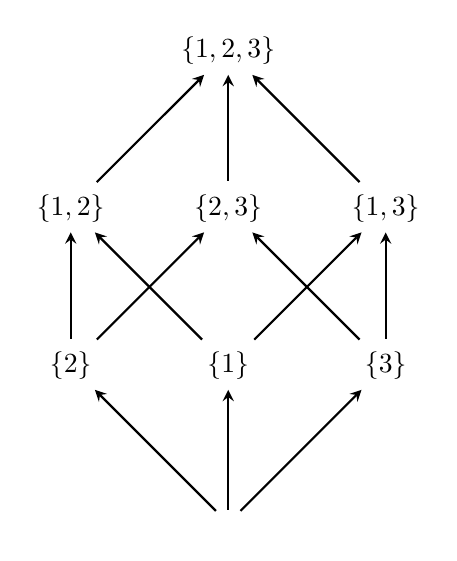
\begin{tikzpicture}[<-,>=stealth,shorten >=1pt,auto,node distance=2cm,thick,main node/.style={scale=0.9,circle,draw,font=\sffamily\normalsize}]
            \node[] (1) {$\{1,2,3\}$};
            \node[] (2)[below of = 1] {$\{2,3\}$};
            \node[] (3)[left of = 2] {$\{1,2\}$};
            \node[] (4)[right of = 2] {$\{1,3\}$};

            \node[] (5)[below of = 2] {$\{1\}$};
            \node[] (6)[below of = 3] {$\{2\}$};
            \node[] (7)[below of = 4] {$\{3\}$};
            \node[] (8)[below of = 5] {$\varnothing$};


            \path[every node/.style={font=\sffamily\small}]
                (1) edge (2)
                (1) edge (3)
                (1) edge (4)

                (2) edge (6)
                (2) edge (7)
                (3) edge (5)
                (3) edge (6)
                (4) edge (5)
                (4) edge (7)

                (5) edge (8)
                (6) edge (8)
                (7) edge (8)
                ;
        \end{tikzpicture}

        \caption{Diagramma di Hasse dell'ordine $\subseteq$ sull'insieme $\mathcal{P}(\{1,2,3\}$)}
    \end{figure}

    Notiamo però una principale differenza tra le relazioni $\leq$ e $\subseteq$. Presi due numeri $n,m \in \N$, abbiamo sempre che $n \leq m$ o che $m \leq n$. In altre parole, ogni elemento può o raggiungere o essere raggiunto da ogni altro elemento. Presi due insiemi $Y,Y' \in \mathcal{P}(X)$, invece, potrebbe tranquillamente verificarsi che i due insiemi siano \textbf{incomparabili}, ossia $Y \not\subseteq Y'$ e $Y' \not\subseteq Y$. Nel primo caso, l'ordine viene detto \textbf{totale} (o \textit{lineare}, per via della forma assunta dal suo diagramma di Hasse), mentre nel secondo caso esso viene detto \textbf{parziale}.

    \begin{frameddefn}{Ordine totale e parziale}
        Sia $\preceq \, \subseteq A \times A$ una relazione d'ordine. Tale ordine viene detto totale se per ogni $a,b \in A$ si ha che almeno una tra $a \preceq b$ e $b \preceq a$ sia valida. Un ordine non totale viene detto parziale.
    \end{frameddefn}

    Gli ordni totali permettono di confrontare gli elementi di un insieme finito in modo del tutto lineare, partendo dal minimo e procedendo seguendo l'ordine. Questo risulta comodo anche dal punto di vista informatico/algoritmico. Gli ordini parziali sono in linea di massima più complicati perchè rendono necessario seguire i diversi \curlyquotes{percorsi ramificati} che collegano gli elementi. Risulta dunque interessante osservare che è sempre possibile estendere un ordine parziale a un ordine totale sullo stesso insieme. Per dimostrare tale risultato, è sufficiente dimostrare il seguente lemma.

    \begin{framedlem}{}
        Sia $\preceq \, \subseteq A \times A$ una relazione d'ordine parziale. Dati due elementi $a,b \in A$ incomparabili, ossia $a \not\preceq b$ e $b \not\preceq a$, esiste una relazione $\preceq^* \subseteq A \times A$ tale che:
        \begin{itemize}
            \item $\preceq \; \subseteq \; \preceq^*$, ossia tale da estendere $\preceq$
            \item $a \preceq^* b$, ossia in grado di comparare $a$ e $b$
            \item $\preceq^*$ è un ordine parziale
        \end{itemize}
    \end{framedlem}


    \begin{proof}
        Dati i due elementi incomparabili $a,b \in A$, definiamo $X$ come l'insieme degli elementi che vengono prima di $a$ in base a $\preceq$. Similmente, definiamo $Y$ come l'insieme degli elementi che vengono dopo $b$ in base a $\preceq$.
        \[X = \{x \in A \mid x \preceq a\} \qquad\qquad Y = \{y \in A \mid b \preceq y\}\]

        Essendo $a$ e $b$ incomparabili per ipotesi, abbiamo che $X \cap Y = \varnothing$: se esistesse un elemento in comune tra i due insiemi, per transitività di $\preceq$ otterremmo che $a \preceq b$, il che è impossibile.

        Consideriamo quindi la relazione $\preceq^* \; =\; \preceq \cup \; (X \times Y)$. Per definizione stessa di $\preceq^*$, abbiamo chiaramente che $\preceq \; \subseteq \; \preceq^*$. Osserviamo inoltre che $a \in X$ e $b \in Y$ per via della riflessività di $\preceq$ implicando quindi $(a,b) \in X \times Y \subseteq \preceq^*$.

        Ci resta quindi da dimostrare solo che $\preceq^*$ sia un ordine parziale. Prima di tutto, osserviamo facilmente che $\preceq^*$ sia riflessiva in quanto $\preceq^*$ è già riflessiva.
        
        Procediamo quindi dimostrando che sia anti-simmetrica. Supponiamo di avere due elementi $x,y \in A$ tali che $x \preceq^* y$ e $y \preceq^* x$. Per definizione di $\preceq^*$, abbiamo quattro casi:
        \begin{enumerate}
            \item $x \preceq y$ e $y \preceq x$. In questo caso, essendo $\preceq$ anti-simmetrica, concludiamo immediatamente che $x = y$.
            \item $x \preceq y$ e $(y,x) \in X \times Y$. Poiché $y \in X$, sappiamo che $y \preceq a$. Ma allora, per transitività di $\preceq$ abbiamo che $x \preceq a$, il che implica che $x \in X$. Tuttavia, per ipotesi abbiamo che $(y,x) \in X \times Y$, dunque $x \in Y$, contraddicendo il fatto che $X \cap Y = \varnothing$.
            \item $(x,y) \in X \times Y$ e $y \preceq x$. Poiché $y \in Y$, sappiamo che $b \preceq y$. Ma allora, per transitività di $\preceq$ abbiamo che $b \preceq x$, il che implica che $x \in Y$. Tuttavia, per ipotesi abbiamo che $(x,y) \in X \times Y$, dunque $x \in X$, contraddicendo il fatto che $X \cap Y = \varnothing$.
            \item $(x,y) \in X \times Y$ e $(y,x) \in X \times Y$. Questo caso è impossibile poiché contraddice direttamente il fatto che $X \cap Y = \varnothing$
        \end{enumerate}

        Dunque, tra i quattro casi solo il primo risulta essere possibile, concludendo che $\preceq^*$ sia anti-simmetrica. Procedendo in modo analogo, è possibile dimostare come essa sia anche transitiva (esercizio), concludendo quindi che sia un ordine.
    \end{proof}

    \begin{framedthm}{Estendibilità ad ordine totale}
        Ogni ordine parziale su un insieme finito $A$ può essere esteso in un ordine totale.
    \end{framedthm}

    \begin{proof}
        Applicare ripetutamente il lemma finché tutti gli elementi di $A$ non sono comparabili tra loro. 
    \end{proof}

    Gli ordini (parziali e totali) godono di molte proprietà intuitive. Ad esempio, essi non contengono \textit{cicli}, ossia cammini che iniziano e finiscono sullo stesso elemento, fatta eccezione dei cicli di lunghezza 1 (i quali sono dati dalla riflessività).

    \begin{framedprop}{}
        Un ordine non contiene cicli di lunghezza maggiore di 1.
    \end{framedprop}

    \begin{proof}
        Sia $\preceq$ un ordine. Supponiamo per assurdo che esista un ciclo $a_1 \preceq a_2 \preceq \ldots \preceq a_k \preceq a_1$ di lunghezza maggiore di 1. Poiché la lunghezza del ciclo è maggiore di 1, deve esserci almeno un elemento $a_i$ tale che $a_1 \neq a_i$. Tuttavia, per transitività di $\preceq$ le catene $a_1 \preceq a_2 \preceq \ldots \preceq a_{i-1} \preceq a_i$ e $a_i \preceq a_{i+1} \preceq \ldots \preceq a_k \preceq a_1$ implicano che $a_1 \preceq a_i$ e che $a_i \preceq a_1$. Ma allora, per anti-simmetria di $\preceq$, ciò può accedere solo se $a_1 = a_i$, generando una contraddizione. Per tanto, tale ciclo non può esistere.
    \end{proof}
    
    Vediamo ora un altro concetto molto intuitiva delle relazioni d'ordine, entrambe usate quotidianamente.
    
    \begin{frameddefn}{Elemento minimo e minimale}
        Sia $\preceq \, \subseteq A \times A$ un ordine. Dato un elemento $a \in A$, diciamo che è:
        \begin{itemize}
            \item \textbf{minimo} se per ogni elemento $b \in A$ vale che $a \preceq b$.
            \item \textbf{minimale} se per ogni elemento $b \in A -\{a\}$ vale che $b \not\preceq a$
        \end{itemize}
    \end{frameddefn}

    Osserviamo che vi è una sottile differenza tra i due concetti appena definiti: un elemento è detto \textit{minimo} se ogni altro elemento viene dopo di esso, mentre è detto \textit{minimale} se non vi sono altri elementi che vengono prima di esso. Chiaramente, un elemento minimo è anche minimale: se ogni altro elemento viene dopo di esso, non potranno esserci elementi che vengono prima di esso. Il contrario invece, non è generalmente vero.

    Difatti, è possibile dimostrare che ogni ordine possiede almeno un elemento minimale, ma vi sono alcuni ordini che non possiedono un minimo. Ad esempio, consideriamo l'ordine $\preceq$ definito tramite il seguente diagramma di Hasse:

    \begin{figure}[H]
        \centering
        \begin{tikzpicture}[->,>=stealth,shorten >=1pt,auto,node distance=2cm,thick,main node/.style={scale=0.9,circle,draw,font=\sffamily\normalsize}]
            \node[] (1) {$1$};
            \node[] (3)[above of = 1] {$3$};
            \node[] (4)[above right of = 3] {$4$};
            \node[] (x)[below right of = 4] {};

            \node[] (2)[below of = x] {$2$};
            \node[] (5)[above of = 4] {$5$};

            \path[every node/.style={font=\sffamily\small}]
                (1) edge (3)
                (3) edge (4)
                (2) edge (4)
                (4) edge (5)
            ;
        \end{tikzpicture}

        \caption{Diagramma di Hasse di un ordine senza minimo ma con due minimali.}
    \end{figure}

    Osserviamo che $1$ e $2$ siano due elementi minimali, ma che essi siano incomparabili, rendendo nessuno dei due un minimo. In altre parole, \curlyquotes{ramo} dell'ordine possiede un elemento minimale (dunque vi è sempre almeno un elemento minimale). Aggiungendo la freccia $1 \to 2$ (dunque tutte le coppie dovute all'aggiunta della coppia $(1,2)$), invece, l'elemento $1$ diventerebbe un minimo poiché i due rami vengono uniti tra loro. In altre parole, se c'è un singolo ramo allora il minimale di tale ramo è anche un minimo! 

    \begin{framedprop}{}
        Sia $\preceq \, \subseteq A \times A$ un ordine. Abbiamo che:
        \begin{itemize}
            \item Esiste sempre almeno un elemento minimale.
            \item Se $\preceq$ è totale, esiste sempre un elemento minimo.
            \item Esiste al massimo un elemento minimo.
        \end{itemize} 
    \end{framedprop}

    \begin{proof}
        Dimostriamo i tre punti in ordine. Per il primo punto, sia $a_1 \preceq a_2 \preceq \ldots \preceq a_k$ un cammino di lunghezza massima su $\preceq$. Se $A = \{a_1, a_2, \ldots, a_k\}$ allora concludiamo che $a_1$ è un elemento minimo, dunque anche minimale. Assumiamo quindi che $A \neq \{a_1, a_2, \ldots, a_k\}$, dunque esiste almeno un elemento $a_i$ non coperto dal cammino massimo. Osserviamo come $a_i \not\leq a_1$, poiché altrimenti il cammino non sarebbe massimale. Questo conclude che per ogni elemento $b \in A - \{a_1\}$ si ha che $a_i \not\preceq a_1$, dunque che $a_1$ sia minimale.

        Per il secondo punto, è facile osservare che se l'ordine è totale allora ogni elemento minimale deve essere minimo: siccome ogni coppia di elementi deve essere confrontabile e non possono esserci elementi che vengono prima del minimale, tutti gli elementi devono venire dopo il minimale.

        Infine, per il terzo punto supponiamo che esistano due elementi minimi distinti $m_1$ e $m_2$. Per definizione, abbiamo che $m_1 \preceq m_2$ e $m_2 \preceq m_1$ poiché entrambi vengono prima di tutti gli altri elementi. Ma allora, per anti-simmetria deve valere che $m_1 = m_2$, contraddicendo l'ipotesi che siano distinti.

    \end{proof}

    \addtocontents{toc}{\protect\newpage}

    \chapter{Induzione}

    \section{Il principio di induzione}

    Il \textbf{principio di induzione} è una delle idee più eleganti e potenti della matematica. Tale principio serve per dimostrare che una certa proprietà $P$ è vera per tutti i numeri naturali. L'idea si basa sul verificare due passaggi fondamentali: dimostrare $P$ è vera per il numero $0 \in \N$ e dimostrare che se è vera per un generico $n \in \N$ allora è vera anche per $n+1 \in \N$. Anche se all'inizio può sembrare un po' astratto, il suo funzionamento ricorda molto l'\textit{effetto domino}: se il primo tassello cade e ogni tassello fa cadere il successivo, allora alla fine cadranno tutti. 

    \begin{framedprinc}{Principio di induzione}
        Sia $P$ una proprietà definibile sui numeri naturali. Il principio di induzione stabilisce che per dimostrare che $P(n)$ sia vera per ogni $n \in \N$ è sufficiente eseguire i seguenti tre passi:
        \begin{enumerate}
            \item \textbf{Caso base}: dimostrare che $P(0)$ sia verà
            \item \textbf{Ipotesi induttiva}: assumere che $P(n)$ sia vera per un certo $n > 0$
            \item \textbf{Passo induttivo}: utilizzare l'ipotesi induttiva per dimostrare che anche $P(n+1)$ è verà
        \end{enumerate}
    \end{framedprinc}

    Per capire meglio di cosa si tratta, consideriamo la seguente proprietà: per ogni $n \in \N$ vale che:
    \[0 + 1 + 2 + \ldots + n = \frac{n(n+1)}{2}\]

    Questa proprietà è nota in letteratura come \textbf{somma di Gauss}. Secondo la storia popolare, Carl Friedrich Gauss, uno dei più importanti matematici della storia, avrebbe scoperto il metodo per sommare rapidamente i primi 100 numeri naturali quando aveva solo 7 o 8 anni, durante una lezione a scuola. La versione più popolare racconta che il maestro, per tenere occupata la classe mentre svolgeva altro, impose agli studenti di sommare i primi 100 numeri naturali.

    Naturalmente, il maestro si aspettava che gli studenti sommassero tutti i numeri naturali uno ad uno, richiedendo loro molto tempo. Gauss, invece, notò rapidamente un pattern tra i primi 100 numeri (ignorando lo 0):
    \[1 + 100 = 101 \qquad 2 + 99 = 101 \qquad 3 + 98 = 101 \qquad \ldots \qquad 50 + 51 = 101\]

    Poiché vi sono 50 coppie aventi somma 101, Gauss concluse subito che $50 \cdot 101 = 5050$ fosse la risposta al compito assegnato. Nonostante il lampo di genio, Gauss venne severamente punito con accusa di aver mancato di rispetto al maestro.

    Generalizzando l'idea di Gauss ai primi $n$ numeri, otteniamo $\frac{n}{2}$ coppie aventi somma $n+1$, portando quindi il totale ad essere $\frac{n(n+1)}{2}$. Prima di procedere, riscriviamo la proprietà precedente tramite il \textit{simbolo di sommatoria}, ossia una notazione contratta indicante la somma dei numeri naturali a partire da $0$ fino ad $n$, ossia:
    \[\sum_{i = 0}^n i = 0 + 1 + 2 + \ldots + n\]

    \textit{Nota}: per chi se ne intendesse di programmazione, questa notazione può essere letta come un ciclo for: per ogni valore di $i$ che va da 0 (poiché inizialmente $i = 1$) fino ad $n$, sommiamo il numero $i$.

    Vogliamo quindi dimostrare per induzione che per ogni $n \in \N$ valga che:
    \[\sum_{i = 0}^n i = \frac{n(n+1)}{2}\]
    
    \begin{enumerate}
        \item \textit{Caso base}: osserviamo che
        \[0 = \frac{0(0+1)}{2}\]
        dunque la proprietà è vera per $0 \in \N$
        \item \textit{Ipotesi induttiva}: assumiamo che la proprietà valga per un generico $n \in \N$ tale che $n > 0$
        \item \textit{Passo induttivo}: consideriamo la somma dei primi $n+1$ numeri:
        \[\sum_{i = 0}^{n+1} i = 0 + 1 + 2 +3 + \ldots + n + (n+1)\]
        Osserviamo come tale comma contenga al suo interno la somma dei primi $n$ numeri. Tuttavia, per ipotesi sappiamo che tale somma è uguale a $\frac{n(n+1)}{2}$. Dunque, tramite un po' di manipolazione algebrica otteniamo che:
        \[\begin{split}
            \sum_{i = 0}^{n+1} i & = (n+1) + \sum_{i = 0}^n i \\
            & (n+1) + \underbrace{\sum_{i = 0}^n i}_{\text{Caso $n$}} \\
            & = (n+1) \underbrace{\frac{n(n+1)}{2}}_{\text{Ipotesi ind.}} \\
            & =\frac{2(n+1) + n(n+1)}{2}\\
            & =\frac{(n+1)(n+2)}{2} \\
            & =\frac{(n+1)((n+1)+1)}{2}
        \end{split}\]

        Avendo esplicitato la somma in termini di $n+1$, concludiamo che la proprietà sia vera anche per $n+1$. La validità dei tre passaggi ci permette di concludere che la proprietà valga per ogni $n \in \N$.
    \end{enumerate}

    Il principio di induzione può essere applicato a qualsiasi proprietà associabile ai numeri naturali. Ad esempio, in geometria è ben noto che una \textit{triangolazione} di un poligono convesso, ossia una divisione del poligono in triangoli ottenuta aggiungendo solo linee tra vertici possieda esattamente $n-2$ triangoli, dove $n$ è il numero di lati del poligono.

    \begin{figure}[H]
        \centering
        \includegraphics[scale=0.5]{images/triangolazione.pdf}
        \caption{Un poligono convesso e la sua triangolazione.}
    \end{figure}

    Prima di tutto, osserviamo che affinché un poligono sia convesso esso deve possedere almeno tre lati. Per tanto, $n = 3$ fornisce il nostro caso base. Dimostriamo quindi tale risultato per induzione.
    \begin{enumerate}
    
        \item \textit{Caso base}: un poligono convesso con 3 lati è necessariamente un triangolo, dunque è già triangolato e contiene $1$ triangolo. La proprietà è quindi vera per $3 \in \N$
        \item \textit{Ipotesi induttiva:} assumiamo che la proprietà valga un certo $n \in \N$ tale che $n > 3$, dunque che ogni poligono convesso con $n$ lati abbia una triangolazione con $n-2$ triangoli
        \item \textit{Passo induttivo:} consideriamo un poligono convesso con $n+1$ lati. Presi due vertici del poligono che siano non adiacenti e che abbiano un vertice adiacente in comune, disegniamo una segmento tra di essi. Questo processo divide il poligono di $n+1$ lati in un triangolo e un sotto-poligono di $n$ lati.
        
        Per ipotesi induttiva, quest'ultimo ha una triangolazione con $n-2$ triangoli. Aggiungendo il nuovo triangolo a tale triangolazione, otteniamo una triangolazione del poligono iniziale avente $n-1 = (n+1)-2$ triangoli. La validità dei tre passaggi ci permette di concludere che la proprietà valga per ogni $n \in \N$ tale che $n \geq 3$.
    \end{enumerate}

    \section{Principi equivalenti all'induzione}

    Ovviamente, affinchè \curlyquotes{l'effetto domino} funzioni non è necessario che il caso base sia dimostrato per $0 \in \N$. Difatti, è possibile partire da un qualsiasi valore $k \in \N$. La giustificazione formale di tale generalizzazione è molto semplice: se vogliamo dimostrare che la proprietà $P$ valga per ogni $n \in \N$ con $n \geq k$, possiamo dimostrare tramite induzione che per ogni $m \in \N$ valga la proprietà $Q$ definita come $P(m-k)$. In altre parole, è come se facessimo \curlyquotes{scorrere di $k$ posti} tutti i numeri naturali.

    \begin{framedprinc}{Principio di induzione (caso base generico)}
        Sia $P$ una proprietà definibile sui numeri naturali. Il principio di induzione stabilisce che per dimostrare che $P(n)$ sia vera per ogni $n \in \N$ con $n \geq k$ è sufficiente eseguire i seguenti tre passi:
        \begin{enumerate}
            \item \textbf{Caso base}: dimostrare che $P(k)$ sia verà
            \item \textbf{Ipotesi induttiva}: assumere che $P(n)$ sia vera per un certo $n > k$
            \item \textbf{Passo induttivo}: utilizzare l'ipotesi induttiva per dimostrare che anche $P(n+1)$ è verà
        \end{enumerate}
    \end{framedprinc}

    Vediamo ora un altro esempio con un caso base generico. Vogliamo dimostare per induzione che per ogni $n \geq 4$ vale che $n^2 \leq 2^n$.
    \begin{enumerate}
        \item \textit{Caso base}: osserviamo che $4^2 \leq 2^4$ poiché $4^2 = 16 = 2^4$, dunque la proprietà è vera per $4 \in \N$
        \item \textit{Ipotesi induttiva}: assumiamo che la proprietà valga per un certo $n \in \N$ tale che $n > 4$
        \item \textit{Passo induttivo}: consideriamo la potenza $(n+1)^2$ sviluppando il binomio otteniamo che:
        \[\begin{split}
            (n+1)^2 &= n^2 + 2n + 1\\
            & =\underbrace{n^2}_{\text{Caso $n$}} + 2n + 1 \\
            & \leq \underbrace{2^n}_{\text{Ipotesi ind.}} + 2n + 1 \\
        \end{split}\]

        A questo punto, osserviamo facilmente che $2n +1 \leq 2^n$ per $n \geq 3$ (anche questo risultato è dimostrabile per induzione!), dunque anche nel nostro caso $n > 4$, ottenendo che:
        \[\begin{split}
            (n+1)^2 & \leq 2^n + 2n + 1 \\
            & \leq 2^n + 2^n \\
            & = 2 \cdot 2^n \\
            & = 2^{n+1}
        \end{split}\]

        Avendo esplicitato la disequazione in termini di $n+1$, concludiamo che la proprietà è vera anche per $n+1$. La validità dei tre passaggi ci permette di concludere che la proprietà valga per ogni $n \in \N$ tale che $n \geq 4$.
    \end{enumerate}

    Un'altra veriante del principio di induzione è dato dal così detto \textbf{principio di induzione forte}. In questa variante, è possibile utilizzare un'ipotesi induttiva molto più forte di quella del normale principio di induzione: invece di assumere la tesi per un generico $n \in \N$ che sia maggiore del caso base, assumiamo che essa valga per \underline{tutti} i numeri naturali $m$ compresi tra il caso base ed $n$.

    \begin{framedprinc}{Principio di induzione forte}
        Sia $P$ una proprietà definibile sui numeri naturali. Il principio di induzione stabilisce che per dimostrare che $P(n)$ sia vera per ogni $n \in \N$ con $n \geq k$ è sufficiente eseguire i seguenti tre passi:
        \begin{enumerate}
            \item \textbf{Caso base}: dimostrare che $P(k)$ sia verà
            \item \textbf{Ipotesi induttiva forte}: assumere che $P(m)$ sia vera per ogni $m \in \N$ tale che $k \leq m \leq n$, dove $n \in \N$ e $k < n$ 
            \item \textbf{Passo induttivo}: utilizzare l'ipotesi induttiva per dimostrare che anche $P(n+1)$ è verà
        \end{enumerate}
    \end{framedprinc}

    Intuitivamente, tra la normale induzione e l'induzione forte non vi è alcuna differenza: ogni cosa dimostrabile dal primo è dimostrabile anche dal secondo è viceversa. Difatti, a livello mentale l'unica differenza tra i due principi è l'utilizzo o meno di pezzi del domino precedenti rispetto al penultimo. Tuttavia, in alcuni casi risulta molto più comodo utilizzare la seconda, soprattutto quando si va a lavorare più sotto-oggetti all'interno dell'oggetto in analisi. Per tanto (volendo) si potrebbe utilizzare sempre l'ipotesi induttiva forte invece di quella normale.

    Tipico esempio di tale caso è dato dal \textit{teorema fondamentale dell'aritmetica}, il quale afferma che ogni numero $n \in \N$ con $n \geq 2$ possa essere scritto come prodotto di numeri primi.

    \begin{enumerate}
        \item \textit{Caso base}: per $n = 2$ non dobbiamo dimostrare nulla in quanto $2$ è già primo

        \item \textit{Ipotesi induttiva forte}: assumiamo che la proprietà valga per ogni $n \in \N$ tale che $k < n \leq h$, dove $h \in \N$

        \item \textit{Passi induttivo}: consideriamo il numero $n+1$. Nel caso in cui $n+1$ sia primo, non dobbiamo dimostrare nulla come nel caso base. Nel caso in cui non sia primo, invece, sappiamo che $n+1 = ab$ per qualche coppia di numeri $a,b \in \N$ con $2 \leq a,b \leq n$.
        
        Dunque, dato che $a,b \leq n$, per ipotesi induttiva forte sappiamo che che $a$ e $b$ possono essere scritti come prodotto di numeri primi. Siano qundi $a = p_1 \cdot \ldots \cdot p_i$ e $b = q_1 \cdot \ldots \cdot q_j$ le fattorizzazioni di $a$ e $b$. Moltiplicando tali fattorizzazioni otteniamo la seguente fattorizzazione per $n+1$, concludendo il passo induttivo:
        \[n+1 = p_1 \cdot \ldots \cdot p_i \cdot q_1 \cdot \ldots \cdot q_j\]
    \end{enumerate}

    Oltre alle varianti del principio induttivo, esistono altri principi matematici che sono equivalenti a quest'ultimo, in particolare il \textbf{principio del minimo numero} (o \textit{del buon ordinamento}). Questo principio è estremamente intuitivo: essendo i numeri naturali ordinabili in modo crescente $0, 1, 2, \ldots$, ogni sottoinsieme non vuoto dei numeri naturali deve possere un valore minimo. 

    \begin{framedprinc}{Principio del minimo numero}
        Se $X \subseteq \N$ e $X \neq \varnothing$ allora $X$ possiede un elemento minimo.
    \end{framedprinc}

    \begin{framedthm}{}
        Il principio di induzione e il principio del minimo numero sono equivalenti.
    \end{framedthm}

    \begin{proof}
        Sia $P$ la proprietà che si vuole dimostrare. Assumendo la validità de principio di induzione, dimostriamo tramite esso che ogni sottoinsieme $X \subseteq \N$ di $n \geq 1$ elementi abbia un elemento minimo.
        
        \begin{enumerate}
            \item \textit{Caso base}: se $\abs{X} = 1$ contiene un solo elemento, il quale chiaramente minimo in $X$
            \item \textit{Ipotesi induttiva:} assumiamo che la proprietà $P$ valga per un certo $n \in \N$ tale che $n > 1$
            \item \textit{Passo induttivo}: consideriamo il caso $\abs{X} = n+1$. Preso un elemento qualsiasi $x \in X$, l'insieme $X-\{x\}$ possiede $n$ elementi. Per ipotesi induttiva, esiste un elemento minimo $m$ in $X-\{x\}$. Confrontando $m$ e $x$, possiamo stabilire chi dei due sia l'elemento minimo di $X$, chiudendo il passo induttivo.
        \end{enumerate}

        Questo dimostra che la validità del principio di induzione implica la validità del principio del minimo numero. Viceversa, assumiamo la validità del principio del minimo numero e dimostriamo tramite esso il principio di induzione. Sia $Y$ l'insieme dei numeri naturali che soddisfa $P$:
        \[Y = \{n \in \N \mid P(y) \text{ è vera}\}\]

        Assumiamo le due pre-condizioni del principio di induzione:
        \begin{enumerate}
            \item Esiste un caso base $k \in \N$ per cui $P(k)$ è vera
            \item Per un generico $n > k$, se $P(n)$ è vera allora anche $P(n+1)$ è vera. 
        \end{enumerate}
        Osserviamo che tali due pre-condizioni sono equivalenti a dire che $k \in Y$ e che se $n \in Y$ allora $n+1 \in Y$.
        
        Supponiamo quindi per assurdo che non sia vera la conclusione del principio di induzione, ossia che esista almeno un numero naturale $z \in \N$ per cui $P(z)$ è falsa. Ciò implica che $z \notin Y$ e dunque che l'insieme $\N - Y$ non sia vuoto. Per il principio del minimo numero, esiste un elemento minimo $m \in \N-Y$ tale che $P(m)$ non è vera.
        
        Implicitamente, questo ci dice che per ogni numero più piccolo di $m$ la proprietà $P$ deve essere vera. Per tanto, sappiamo che $P(m-1)$ deve essere vera. Tuttavia, la seconda condizione assunta ci dice che se $P(m-1)$ è vera allora anche $P(m)$ deve essere vera, il che conclude che $m \notin \N-Y$, generando un assurdo. L'unica possibilità è quindi che la conclusione del principio di induzione sia vera, ossia che $Y = \N$. 
    \end{proof}

    Essendo i due principi del tutto equivalenti tra loro, in alcuni casi è possibile utilizzare direttamente il principio del minimo numero. Ad esempio, possiamo dimostrare il \textit{teorema fondamentale dell'aritmetica} anche tramite il principio del minimo numero.

    Sia $X \subseteq \N$ l'insieme dei numeri naturali che sono o minori di 2 o che ammettono una fattorizzazione in numeri primi. Supponiamo per assurdo che $X \neq \N$, ossia che esista almeno un elemento nell'insieme $\N-X$. Per il principio del minimo numero, esiste un elemento minimo $m \in \N-X$.
    
    Poiché $0,1 \in X$, ne segue necessariamente che $m \geq 2$. Inoltre, è impossibile che $m$ sia primo, altrimenti avremmo che $m \in X$. Per tanto, $m$ è un numero composto scrivibile come $m = ab$, dove $2 \leq a,b < m$. Essendo $a$ e $b$ minori di $m$, essi ammettono una fattorizzazione. Siano qundi $a = p_1 \cdot \ldots \cdot p_i$ e $b = q_1 \cdot \ldots \cdot q_j$ le fattorizzazioni di $a$ e $b$. Moltiplicando tali fattorizzazioni otteniamo la seguente fattorizzazione per $m$, il che è assurdo.
    \[m = p_1 \cdot \ldots \cdot p_i \cdot q_1 \cdot \ldots \cdot q_j\]

    Per tanto, ne segue necessariamente che $X = \N$ sia l'unica possibilità. 


    \section{Errori di induzione}

    Nelle sezioni precedenti abbiamo visto come il principio di induzione sia uno strumento molto potente al fine di dimostrare risultati. Ma come disse lo Zio Ben a Peter Parker, \curlyquotes{da un grande potere derivano grandi responsabilità}: bisogna porre estrema attenzione durante lo sviluppo dei vari passaggi del principio, altrimenti potremmo arrivare a dimostrare cose del tutto assurde.

    In alcuni casi, ad esempio, potremmo convincerci della validità di una proprietà ragionando solo ed esclusivamente sul suo passo induttivo, senza curarci della correttezza del caso induttivo. Chiaramente, risulta essere un errore cruciale: è come se avessimo posizionato correttamente tutti i pezzi del domino senza aver tirato la schicchera al pezzo iniziale!

    Nel caso più comune, invece, l'errore è situato nello sviluppo del passo induttivo stesso. Tipicamente, ciò si verifica quando viene posta poca attenzione alle operazioni che si stanno svolgendo, senza accertarsi che esse siano valide per un $n$ generico (dunque che valga anche in casi limite).

    Per comprendere meglio la seconda tipologia di errore, consideriamo il seguente esempio. Discutendo con suo fratello Mario, Luigi afferma che ogni tifoso di calcio tifa una ed una sola squadra: il Catanzaro FC. Dopo essere stato sbeffeggiato dal fratello per la sua affermazione, Luigi tenta di sostenere la correttezza della sua tesi dimostrando per induzione che per ogni insieme di $n$ tifosi, con $n \in \N$ e $n \geq 1$, è vero che ognuno di essi tifa la stessa squadra. Luigi procede quindi col seguente argomento:

    \begin{enumerate}
        \item \textit{Caso base}: considerando un insieme $X = \{t_1\}$ contenente un solo tifoso è chiaro che ogni tifoso di $X$ tifi la stessa squadra, ossia quella tifata da $t_1$

        \item \textit{Ipotesi induttiva}: assumiamo che la proprietà valga per un certo $n > 1$

        \item \textit{Passo induttivo (corretto?)}: dato un insieme $X = \{t_1, \ldots, t_{n+1}\}$ di $n+1$ tifosi, consideriamo i sotto-insiemi $X_1, X_2$ contenenti i primi $n$ tifosi e gli ultimi $n$ tifosi.
        \[X_1 = \{t_1, \ldots, t_n\} \qquad\qquad X_2 = \{t_2, \ldots, t_{n+1}\}\]

        Per ipotesi induttiva, sappiamo che tutti i tifosi di $X_1$ tifano la stessa squadra $S_1$. Analogamente, tutti i tifosi di $X_2$ tifano la squadra $S_2$. Tuttavia, poiché $X_1 \cap X_2 \neq \varnothing$, deve necessariamente valere che $S_1 = S_2$, altrimenti ci sarebbe un tifoso in $X_1$ e in $X_2$ che tifa due squadre, creando una contraddizione. Dunque, concludiamo che tutti i tifosi di $X$ tifano la stessa squadra!
    \end{enumerate}
    
    Dopo aver sentito l'argomento del fratello, Mario scoppia a ridere. Infuriato, Luigi chiede cosa ci sia di sbagliato nella sua dimostrazione. Dopo essersi calmato, Mario osserva come non sia sempre garantita l'esistenza di un tifoso in comune tra $X_1$ e $X_2$. Difatti, quando $n = 2$ abbiamo che $X_1 = \{t_1\}$ e $X_2 = \{t_2\}$, i quali sono completamente disgiunti. Abbattuto, Luigi ammette il suo errore di induzione.

    \section{Rafforzamento dell'ipotesi induttiva}

    Supponiamo di avere un pavimento quadrato composto di $2^n \times 2^n$ quadrati. Vogliamo ricoprire il pavimento con un numero finito piastrelle bianche non scompobibili, ciascuna composta da 3 quadrati a forma di $L$, rispettando il seguente vincolo: uno dei quattro quadrati al centro del pavimento deve essere lasciato vuoto, al fine di essere coperto da una piastrella nera.

    Un arredatore ci assicura che sia possibile farlo per ogni $n \geq 1$. Assendo molto scettici, cerchiamo di dimostrare la sua tesi per induzione.

    \begin{enumerate}
        \item \textit{Caso base}: con un pavimento $2^1 \times 2^1$ abbiamo solo 4 piastrelle, dunque ognuna delle piastrelle è una delle 4 piastrelle centrali. Per tanto, è sufficiente coprire tre quadrati con una piastrella bianca al fine di rispettare il vincolo.
        \begin{figure}[H]
            \centering
            \includegraphics[scale=0.5]{images/induction1.png}
            \caption{Le quattro possibili coperture nel caso base.}
        \end{figure}

        \item \textit{Ipotesi induttiva}: assumiamo che la proprietà valga per un certo $n > 1$
        
        \item \textit{Passo induttivo (o forse no)}: consideriamo un pavimento $2^{n+1} \times 2^{n+1}$. Poiché $2^{n+1} = 2 \cdot 2^{n}$, il pavimento è scomponibile in quattro sotto-pavimenti grandi $2^n \times 2^n$.
        \begin{figure}[H]
            \centering
            \includegraphics[scale=0.6]{images/induction2.png}
            \caption{Scomposizione del pavimento $2^{n+1} \times 2^{n+1}$ nei quattro sotto-pavimenti.}
        \end{figure}

        Per ipotesi induttiva, ognuno di questi quattro sotto-pavimenti è ricopribile lasciando una piastrella centrale vuota. Tuttavia, osserviamo due problemi:
        \begin{enumerate}
            \item Le piastrelle bianche non sono scomponibili, dunque non possiamo coprire i tre buchi senza muovere alcune delle piastrelle già posizionate
            \item Anche se potessimo spostare le piastrelle già posizionale, possiamo aggiungere massimo una piastrella bianca, coprendo massimo 3 dei buchi centrali lasciati dai 4 sotto-pavimenti. Chi ci assicura che il buco rimanente si trovi al centro al centro del pavimento $2^{n+1} \times 2^{n+1}$?
        \end{enumerate}

        Concludiamo quindi che dimostrare il passo induttivo per questa ipotesi sia estremamente difficile.
    \end{enumerate}

    Vista la difficoltà nel chiudere il passo induttivo della dimostrazione, andiamo a lamentarci con l'arredatore riguardo la correttezza della sua affermazione. Dopo una piccola risata, l'arredatore ci suggerisce il suo segreto: l'ipotesi da lui usata è diversa dalla nostra. In particolare, l'arredatore ha utilizzato una ipotesi \textit{più generica} della nostra per dimostrare il caso specifico. Questo concetto è noto come \textbf{rafforzamento dell'ipotesi induttiva} (il quale è \underline{diverso} dal concetto di ipotesi induttiva forte).

    Ancora dubbiosi, chiediamo all'arredatore quale sia la sua ipotesi rafforzata, il quale ci risponde di aver dimostrato che sia possibile riempire il pavimento $2^{n+1} \times 2^{n+1}$ lasciamo un quadrato vuoto in uno spazio \underline{qualsiasi} e non strettamente al centro del pavimento. Questa piccola variazione ci permette di rendere l'ipotesi induttiva più generica, permettendoci di scegliere dove si trovino i 4 buchi dei sotto-pavimenti.

    \begin{enumerate}
        \item \textit{Caso base:} identico al tentativo precedente
        \item \textit{Ipotesi induttiva}: assumiamo che la proprietà \textit{rafforzata} valga per un certo $n > 1$
        \item \textit{Passo induttivo}: consideriamo un pavimento $2^{n+1} \times 2^{n+1}$. Poiché $2^{n+1} = 2 \cdot 2^{n}$, il pavimento è scomponibile in quattro sotto-pavimenti grandi $2^n \times 2^n$.
        
        Sia $P$ una qualsiasi posizione vuota che vogliamo lasciare nel pavimento $2^{n+1} \times 2^{n+1}$. Per ipotesi induttiva, ognuno dei questi quattro sotto-pavimenti è ricopribile lasciando un qualsiasi quadrato vuoto. In particolare, per il sotto-pavimento contenente la posizione $P$ scegliamo di lasciare vuota proprio quella posizione, mentre per gli altri 3 sotto-pavimenti lasciamo vuota la posizione che tocca il centro del sovra-pavimento.

        \begin{figure}[H]
            \centering
            \includegraphics[scale=0.6]{images/induction3.png}
            \caption{Utilizzo dell'ipotesi induttiva rafforzata sui 4 sotto-pavimenti}
        \end{figure}

        Chiaramente gli spazi vuoti dei 3 sotto-pavimenti possono essere coperti da una piastrella bianca, lasciando la posizione $P$ l'unica scoperta nel pavimento $2^{n+1} \times 2^{n+1}$. Questo conclude correttamente il passo induttivo.
    \end{enumerate}

    \newpage



    \chapter{Logica proposizionale}

    \section{Introduzione ai costrutti logici}

    La logica si occupa della validità del ragionamento indipendentemente dal significato dei suoi componenti. In particolare, la \textbf{logica proposizionale} si occupa dello studio delle proprietà di determinati costrutti logici utilizzati nel linguaggio naturale così come nella pratica scientifica e matematica. In particolare, ci interessano i seguenti costrutti:
    \begin{itemize}
        \item \textit{Negazione} (\( \neg \)):  inverte il valore di verità di una proposizione. Se una proposizione è vera, la sua negazione è falsa, e viceversa.
        \item \textit{Congiunzione} (\( \wedge \)):  rappresenta il connettivo logico \textit{e}. Il risultato è vero se e solo se entrambi i componenti sono veri.
        \item \textit{Disgiunzione} (\( \vee \)):  rappresenta il connettivo logico \textit{oppure}. Il risultato è vero se almeno uno dei componenti è vero.
        \item \textit{Implicazione} (\( \to \)):  rappresenta l'enunciato logico \textit{se \dots allora}. Il risultato è falso solo se il primo componente è vero e il secondo componente è falso. In altre parole, questo operatore impone che quando la premessa è vera, la conclusione deve sempre seguire (se la premessa è falsa, non ci interessa la veridicità della conclusione).
        \item \textit{Equivalenza} (\( \liff \)):  rappresenta l'enunciato logico \textit{se e solo se}. Il risultato è vero quando entrambi i componenti hanno lo stesso valore di verità, cioè sono entrambi veri o entrambi falsi.
    \end{itemize}

    Ad esempio, consideriamo il seguente semplice argomento aritmetico:
    \begin{enumerate}
        \item Se \( a = 0 \) o \( b = 0 \), allora \( a \cdot b = 0 \)
        \item \( a \cdot b \neq 0 \)
        \item \( a \neq 0 \) e \( b \neq 0 \)
    \end{enumerate}

    Intuitivamente, la terza proposizione \textit{segue} dalle altre due proposizioni, cioè è la conclusione di un argomento con le prime due come premesse. Per formalizzare questo argomento, prima identifichiamo quelle parti che non possono essere ulteriormente analizzate in termini di costrutti logici e che possono essere vere o false (chiamate \textbf{parti atomiche}). Nel nostro caso, queste parti atomiche sono \( a = 0 \), \( b = 0 \), e \( a \cdot b = 0 \).

    Assegniamo una lettera distinta a ciascuna di queste parti atomiche: per \( a = 0 \), associamo \( A \); per \( b = 0 \), associamo \( B \); e per \( a \cdot b = 0 \), associamo \( C \). Poi, sostituamo i costrutti logici nel linguaggio naturale (se \dots allora, oppure, e, non) con simboli formali, chiamati connettivi booleani: \( \neg \) per la negazione, \( \vee \) per la disgiunzione, \( \wedge \) per la congiunzione, \( \rightarrow \) per l'implicazione (se \dots allora), e \( \leftrightarrow \) per l'equivalenza (se e solo se).

    Otteniamo la seguente formalizzazione:
    \begin{enumerate}
        \item $(A \lor B) \to C$
        \item $\lnot C$
        \item $\lnot A \land \lnot B$
    \end{enumerate}

    dove leggiamo \( A \lor B \) come \textit{A oppure B}, \( \neg C \) come \textit{non C} e così via. Consideriamo ora il seguente argomento verbale:
    \begin{enumerate}
        \item Se il padre è alto o la madre è alta, allora il bambino è alto
        \item Il bambino è basso
        \item Il padre è basso e la madre è bassa
    \end{enumerate}

    Se tentiamo una formalizzazione dell'argomento, ci rendiamo rapidamente conto che otteniamo la stessa formalizzazione dell'argomento precedente, dove scriviamo \( A \) per \textit{il padre è alto}, \( B \) per \textit{la madre è alta}, e \( C \) per \textit{il bambino è alto}. Pertanto, i due argomenti sono identici. La logica formale ci consente di identificare la struttura logica comune in argomenti che trattano oggetti e strutture differenti, come nel caso degli esempi sopra. Tuttavia, in questo caso, la prima premessa è ovviamente nota per essere empiricamente falsa. Tuttavia, se la assumiamo come premessa per un argomento, riconosciamo intuitivamente che il ragionamento è \textbf{valido} (o corretto). Quando diciamo che l'argomento è valido (o corretto), intendiamo che se le premesse sono vere, allora la conclusione è anche vera; \underline{non} che le premesse siano vere.

    Per valutare la veridicità di una proposizione, utilizziamo le \textbf{tavole di verità}. In logica, una tavola di verità è una tabella utilizzata per determinare se un'espressione logica è vera o falsa in base ai \textbf{valori di verità} dei suoi componenti. Le tavole di verità sono utilizzate principalmente per valutare la validità delle proposizioni logiche e determinare le relazioni tra le varie proposizioni logiche. Ogni riga di una tavola di verità rappresenta una combinazione unica di valori di verità per le variabili coinvolte nell'espressione logica. Le colonne mostrano i valori di verità intermedi dei componenti dell'espressione, portando infine alla valutazione dell'intera formula logica.

    \begin{figure}[H]
        \centering
        \begin{tabular}{c c c c c}
            \begin{tabular}{c|c}
                $A$ & $\lnot A$ \\
                \hline
                0 & 1 \\
                1 & 0
            \end{tabular}

            & \qquad \qquad &

            \begin{tabular}{cc|c}
                $A$ & $B$ & $A \land B$ \\
                \hline
                0 & 0 & 0 \\
                0 & 1 & 0 \\
                1 & 0 & 0 \\
                1 & 1 & 1 \\
            \end{tabular}

            & \qquad \qquad &

            \begin{tabular}{cc|c}
                $A$ & $B$ & $A \lor B$ \\
                \hline
                0 & 0 & 0 \\
                0 & 1 & 1 \\
                1 & 0 & 1 \\
                1 & 1 & 1 \\
            \end{tabular}
        \end{tabular}

        \vspace{15pt}

        \begin{tabular}{c c c}
            \begin{tabular}{cc|c}
                $A$ & $B$ & $A \to B$ \\
                \hline
                0 & 0 & 1 \\
                0 & 1 & 1 \\
                1 & 0 & 0 \\
                1 & 1 & 1 \\
            \end{tabular}

            & \qquad \qquad &

            \begin{tabular}{cc|c}
                $A$ & $B$ & $A \liff B$ \\
                \hline
                0 & 0 & 1 \\
                0 & 1 & 0 \\
                1 & 0 & 0 \\
                1 & 1 & 1 \\
            \end{tabular}
        \end{tabular}

        \caption{tavole di verità dei cinque operatori logici precedentemente introdotti. Il valore 0 rappresenta la falsità delle proposizioni, mentre il valore 1 rappresenta la loro veridicità.}
    \end{figure}

    Consideriamo ora un'espressione logica più complessa \( A \rightarrow (B \wedge C) \). Una tavola di verità per questa richiede la valutazione dei valori di verità per \( A \), \( B \) e \( C \), quindi determinando il valore di verità della congiunzione \( B \wedge C \), e infine quello di \( A \rightarrow (B \wedge C) \).

    \begin{figure}[H]
        \centering
        
        \begin{tabular}{ccc|c|c}
            \( A \) & \( B \) & \( C \) & \( B \wedge C \) & \( A \rightarrow (B \wedge C) \) \\
            \hline
            0 & 0 & 0 & 0 & 1 \\
            0 & 0 & 1 & 0 & 1 \\
            0 & 1 & 0 & 0 & 1 \\
            0 & 1 & 1 & 1 & 1 \\
            1 & 0 & 0 & 0 & 0 \\
            1 & 0 & 1 & 0 & 0 \\
            1 & 1 & 0 & 0 & 0 \\
            1 & 1 & 1 & 1 & 1 \\
        \end{tabular}

        \label{form_1}
        \caption{Tavola di verità per l'espressione logica \( A \rightarrow (B \wedge C) \)}
    \end{figure}

    \section{Formalizzazione matematica}

    Il primo passo è definire un linguaggio formale completamente rigoroso che possa essere sottoposto a studio matematico. Per la logica proposizionale, la procedura è semplice: le proposizioni sono formalizzate da formule ottenute applicando i connettivi booleani ad alcuni blocchi atomici, chiamati \textit{variabili proposizionali}. Queste variabili rappresentano intuitivamente proposizioni che non possono essere ulteriormente analizzate in termini di operatori logici come negazione, congiunzione, disgiunzione, implicazione o equivalenza.

    \begin{frameddefn}{Linguaggio e proposizioni}
        Un linguaggio proposizionale è un insieme $\mathcal{L} = \{p_1, \ldots, p_n\}$, dove ciascun $p_i$ è un simbolo chiamato variabile proposizionale. Dato un linguaggio proposizionale $\mathcal{L}$, l'insieme delle proposizioni (o formule valide) su $\mathcal{L}$, denotato con $\mathsf{PROP}_\mathcal{L}$ (o $\mathsf{FML}_\mathcal{L}$), è l'insieme minimo di espressioni finite su $\mathcal{L} \cup \{\lnot, \land, \lor, \to, \liff\}$ tale che:
        \begin{itemize}
            \item Ogni variabile proposizionale in $\mathcal{L}$ è una proposizione, cioè $\mathcal{L} \subseteq \mathsf{PROP}_\mathcal{L}$
            \item Se $A \in \mathsf{PROP}_\mathcal{L}$ allora $\lnot A \in \mathsf{PROP}_\mathcal{L}$
            \item Se $A, B \in \mathsf{PROP}_\mathcal{L}$ allora $(A \land B), (A \lor B), (A \to B), (A \liff B) \in \mathsf{PROP}_\mathcal{L}$
        \end{itemize}
    \end{frameddefn}
    
    Quando $\mathcal{L}$ è non ambiguo nel contesto, denotiamo $\mathsf{PROP}_\mathcal{L}$ direttamente come $\mathsf{PROP}$. Inoltre, per rendere le espressioni più facili da leggere, utilizziamo le seguenti regole di precedenza: $\lnot$ ha precedenza su $\land, \lor$, mentre $\land, \lor$ hanno precedenza su $\to, \liff$. In altre parole, abbiamo che $(\lnot((\lnot A) \lor B)) \to C$ può essere scritto come $\lnot(\lnot A \lor B) \to C$.
    
    Dopo aver formalizzato il concetto di linguaggio proposizionale e proposizioni, siamo pronti a formalizzare il concetto di tabelle di verità. Ogni riga di una tabella di verità può essere descritta attraverso \textbf{assegnamenti}. Un assegnamento è una funzione $\alpha : \mathcal{L} \to \{0,1\}$, cioè una mappa che assegna un valore di verità a ciascuna variabile proposizionale del linguaggio. Per estensione, ogni assegnamento su $\mathcal{L}$ induce un assegnamento su $\mathsf{PROP}$. Questi assegnamenti sono funzioni $\widehat{\alpha} : \mathsf{PROP} \to \{0,1\}$ definite in modo induttivo come:
    \[
    \widehat{\alpha}(A) = \alpha(A) \text{ quando } A \in \mathcal{L}
    \]
    \[
    \widehat{\alpha}(\lnot A) = \soe{ll}{
        1 & \text{se } \widehat{\alpha}(A) = 0 \\
        0 & \text{se } \widehat{\alpha}(A) = 1 \\
    }
    \]
    
    \[
    \widehat{\alpha}(A \land B) = \soe{ll}{
        1 & \text{se } \widehat{\alpha}(A) = \widehat{\alpha}(B) = 1 \\
        0 & \text{altrimenti} \\
    }
    \]
    
    \[
    \widehat{\alpha}(A \lor B) = \soe{ll}{
        0 & \text{se } \widehat{\alpha}(A) = \widehat{\alpha}(B) = 0 \\
        1 & \text{altrimenti} \\
    }
    \]
    
    \[
    \widehat{\alpha}(A \to B) = \soe{ll}{
        0 & \text{se } \widehat{\alpha}(A) = 1 \text{ e } \widehat{\alpha}(B) = 0 \\
        1 & \text{altrimenti} \\
    }
    \]
    
    \[
    \widehat{\alpha}(A \liff B) = \soe{ll}{
        1 & \text{se } \widehat{\alpha}(A) = \widehat{\alpha}(B) \\
        0 & \text{altrimenti} \\
    }
    \]
    
    Per semplificare la notazione, ci riferiremo direttamente a $\widehat{\alpha}$ come $\alpha$. Utilizzando il concetto di assegnamenti, possiamo anche definire il concetto di \textbf{equivalenza logica}. Informalmente, due formule si dicono logicamente equivalenti quando condividono la stessa tabella di verità.
    
    \begin{frameddefn}{Equivalenza logica}
        Diciamo che due formule $A, B \in \mathsf{PROP}$ sono logicamente equivalenti, denotate con $A \equiv B$, quando per ogni assegnamento $\alpha$ vale che $\alpha(A) = \alpha(B)$.
    \end{frameddefn}
    
    Per definizione, è chiaro che $\equiv$ è una relazione d'equivalenza poiché è riflessiva, simmetrica e transitiva. Le equivalenze logiche ci permettono di trattare i componenti logici come se fossero operatori algebrici. Ad esempio, le proprietà algebriche comuni includono:
    \begin{itemize}
        \item \textit{Involuzione}: $\lnot \lnot A \equiv A$
        \item \textit{Idempotenza}: $A \lor A \equiv A$ e $A \land A \equiv A$
        \item \textit{Associatività}: $(A \lor B) \lor C \equiv A \lor (B \lor C)$ e $(A \land B) \land C \equiv A \land (B \land C)$
        \item \textit{Commutatività}: $A \lor B \equiv B \lor A$ e $A \land B \equiv B \land A$
        \item \textit{Distributività}:  $A \lor (B \land C) \equiv (A \lor B) \land (A \lor C)$ e $A \land (B \lor C) \equiv (A \land B) \lor (A \land C)$
        \item \textit{Legge di De Morgan}: $\lnot(A \lor B) \equiv \lnot A \land \lnot B$ e $\lnot(A \land B) \equiv \lnot A \lor \lnot B$
    \end{itemize}
    
    Attraverso queste proprietà di base, notiamo che ogni connettivo può essere riscritto in termini degli altri connettivi. Infatti, potremmo definire la logica proposizionale usando solo $\lnot$ e $\land$ (o $\lnot$ e $\lor$). Questa proprietà è molto utile nella logica dei circuiti.
    \begin{itemize}
        \item $A \land B \equiv \lnot(\lnot A \lor \lnot B)$
        \item $A \lor B \equiv \lnot(\lnot A \land \lnot B)$
        \item $A \to B \equiv \lnot A \lor B$
        \item $A \liff B \equiv (A \to B) \land (B \to A)$
    \end{itemize}
    
    Se per un assegnamento $\alpha$ e una formula $A$ vale che $\alpha(A) = 1$, diciamo che $\alpha$ \textit{soddisfa} $A$. Se $A$ ha almeno un assegnamento soddisfacente, diciamo che $A$ è \textbf{soddisfacibile}. Quando non esiste alcun assegnamento soddisfacente, diciamo che la formula $A$ è \textbf{insoddisfacibile}. Al contrario, quando ogni possibile assegnamento soddisfa $A$, diciamo che $A$ è una \textbf{tautologia} (o \textit{verità logica}, \textit{valida logicamente}). Per definizione, le tautologie rappresentano affermazioni che sono sempre vere, indipendentemente dalla situazione. Denotiamo con $\mathsf{SAT}, \mathsf{UNSAT}$ e $\mathsf{TAUT}$ gli insiemi di formule soddisfacibili, insoddisfacibili e tautologiche. Per definizione, abbiamo che $F \in \mathsf{TAUT}$ se e solo se $\lnot F \in \mathsf{UNSAT}$.
    Se una formula non è una tautologia, non possiamo garantire la veridicità dell'affermazione. Pertanto, consideriamo \textit{affermazioni vere} solo come formule che sono \textit{sempre vere} (l'insieme $\mathsf{TAUT}$), mentre consideriamo \textit{affermazioni false} come formule che \textit{non sono sempre vere} (l'insieme $\mathsf{UNSAT} \cup (\mathsf{SAT} - \mathsf{TAUT})$).

    Con un lieve abuso di notazione, definiamo $1$ e $0$ come le formule tali che, per ogni assegnamento, si ha che $\alpha(1) = 1$ e $\alpha(0) = 0$. Questo ci permette di semplificare ulteriormente le equivalenze logiche algebricamente:
    \begin{itemize}
        \item \textit{Legge di assorbimento}: $A \lor 0 \equiv A$ e $A \land 1 \equiv A$
        \item \textit{Legge di cancellazione}: $A \lor 1 \equiv 1$ e $A \land 0 \equiv 0$
        \item \textit{Tertium non datur}: $A \lor \lnot A \equiv 1$ e $A \land \lnot A \equiv 0$
    \end{itemize}

    Usando tutte le regole algebriche che abbiamo mostrato, possiamo facilmente valutare le formule proposizionali riducendole prima a una formula equivalente più piccola e poi (eventualmente) valutando la tavola della verità della forma ridotta:
    \[
    \begin{split}
        A \lor B \to B \lor \lnot C &\equiv \lnot (A \lor B) \lor B \lor \lnot C \\
        & \equiv (\lnot A \land \lnot B) \lor B \lor \lnot C \\
        & \equiv ((\lnot A \lor B) \land (\lnot B \lor B)) \lor \lnot C \\
        & \equiv ((\lnot A \lor B) \land 1) \lor \lnot C \\
        & \equiv \lnot A \lor B \lor \lnot C \\
    \end{split}
    \]

    I concetti di tautologia e insoddisfacibilità sono strettamente legati al concetto di \textbf{conseguenza logica} che abbiamo discusso nella sezione precedente.

    \begin{frameddefn}{Conseguenza logica}
        Date le formule $A_1, \ldots, A_n, A$, diciamo che $A$ è una conseguenza logica di $A_1, \ldots, A_n$, scritto come $A_1, \ldots, A_n \models A$, se ogni volta che $A_1, \ldots, A_n$ sono vere, anche $A$ è vera.
    \end{frameddefn}

    Attraverso le tavole della verità, valutare se possiamo concludere $A$ da $A_1, \ldots, A_n$ è abbastanza semplice: $A_1, \ldots, A_n \models A$ se e solo se per ogni riga in cui $A_1, \ldots, A_n$ sono valutate come 1, anche $A$ è valutata come 1. Per esempio, consideriamo il problema della \textit{partita dei logici}, costituito dalle seguenti proposizioni:
    \begin{enumerate}
        \item Se la partita dei logici vince le elezioni, allora le tasse aumenteranno se il deficit rimane elevato
        \item Se la partita dei logici vince le elezioni, il deficit rimane elevato
        \item Se la partita dei logici vince le elezioni, le tasse aumenteranno
    \end{enumerate}

    Vogliamo sapere se l'ultima proposizione è una conseguenza logica delle altre due proposizioni. Prima, definiamo le seguenti variabili proposizionali:
    \begin{itemize}
        \item Sia $P$ la variabile tale che $P = 1$ se e solo se la partita dei logici vince le elezioni
        \item Sia $T$ la variabile tale che $T = 1$ se e solo se le tasse aumenteranno
        \item Sia $D$ la variabile tale che $D = 1$ se e solo se il deficit rimane elevato
    \end{itemize}

    Usando le tre variabili, formalizziamo le tre proposizioni come segue:
    \begin{enumerate}
        \item $P \to (D \to T) \equiv \lnot P \lor (\lnot D \lor T) \equiv \lnot P \lor \lnot D \lor T$ 
        \item $P \to D \equiv \lnot P \lor D$
        \item $P \to T \equiv \lnot P \lor T$
    \end{enumerate}

    \newpage

    Poi, calcoliamo la tavola della verità per il problema:
    \begin{figure}[H]
        \centering
        \begin{tabular}{ccc|cc|c}
            $P$ & $T$ & $D$ & $\lnot P \lor \lnot D \lor T$ & $\lnot P \lor D$ & $\lnot P \lor T$ \\
            \hline
            0 & 0 & 0 & 1 & 1 & 1 \\
            0 & 0 & 1 & 1 & 1 & 1 \\
            0 & 1 & 0 & 1 & 1 & 1 \\
            0 & 1 & 1 & 1 & 1 & 1 \\
            1 & 0 & 0 & 1 & 0 & 0 \\
            1 & 0 & 1 & 1 & 0 & 1 \\
            1 & 1 & 0 & 0 & 1 & 0\\
            1 & 1 & 1 & 1 & 1 & 1\\
        \end{tabular}
        \label{form_1}
        \caption{Tavola della verità per il problema della partita dei logici.}
    \end{figure}

    Osserviamo che per ogni assegnamento $\alpha$ tale che $\alpha(P \to (D \to T)) = 1$ e $\alpha(P \to D) = 1$, si ha anche che $\alpha(P \to T) = 1$. Pertanto, possiamo effettivamente concludere che $P \to (D \to T), P \to D \models P \to T$. Poiché il numero di righe in una tavola della verità è esponenziale rispetto al numero di variabili proposizionali, enumerare l'intera tavola della verità potrebbe essere troppo costoso. Ad esempio, con solo $4$ variabili dovremmo enumerare $2^4 = 16$ righe. Per aiutare con questo problema, il seguente teorema è molto utile.

    \begin{framedthm}{}
        Date le formule $A_1, \ldots, A_n, A$, i seguenti tre enunciati sono equivalenti:
        \begin{enumerate}
            \item  $A_1, \ldots, A_n \models A$
            \item  $(A_1 \land \ldots \land A_n \to A) \in \mathsf{TAUT}$
            \item  $(A_1 \land \ldots \land A_n \land \lnot A) \in \mathsf{UNSAT}$
        \end{enumerate}
    \end{framedthm}

    \begin{proof} Omesso (si consiglia di provare a dimostrarlo per prendere confidenza con i tre concetti, la dimostrazione è molto semplice)
    \end{proof}

    Pertanto, per valutare se $A_1, \ldots, A_n \models A$ è valido, possiamo dimostrare che $(A_1 \land \ldots \land A_n \to A) \equiv 1$ oppure che $(A_1 \land \ldots \land A_n \land \lnot A) \equiv 0$ tramite le proprietà algebriche mostrate in precedenza.

    Per esempio, consideriamo il problema del \textit{pulsante di autodistruzione}. Dobbiamo viaggiare lontano nella galassia e Adam ci presta la sua navetta spaziale. Adam ci dice che la navetta ha tre pulsanti e che uno e solo uno di essi attiva il protocollo di autodistruzione, mentre gli altri non fanno nulla. Inoltre, ciascuno dei tre pulsanti ha un post-it attaccato. Il primo e il secondo pulsante dicono \curlyquotes{Non sono il pulsante di autodistruzione}, mentre il terzo pulsante dice \curlyquotes{Il primo pulsante è il pulsante di autodistruzione}. Adam ci dice che uno e solo uno dei pulsanti dice la verità. Usando la logica pura, dobbiamo scoprire quale pulsante è quello di autodistruzione per evitare di farci esplodere.

    Prima, definiamo tre variabili proposizionali:
    \begin{itemize}
        \item Sia $A$ la variabile tale che $A = 1$ se e solo se il primo pulsante attiva il protocollo di autodistruzione
        \item Sia $B$ la variabile tale che $B = 1$ se e solo se il secondo pulsante attiva il protocollo di autodistruzione
        \item Sia $C$ la variabile tale che $C = 1$ se e solo se il terzo pulsante attiva il protocollo di autodistruzione
    \end{itemize}

    Poi, formalizziamo l'intero problema attraverso le seguenti due proposizioni $\phi, \psi$:
    \begin{enumerate}
        \item Uno e solo uno dei pulsanti attiva il protocollo di autodistruzione, cioè
        \[
        \phi = (A \lor B \lor C) \land \lnot (A \land B) \land \lnot (A \land C) \land \lnot (B \land C)
        \]
        \item Uno e solo uno dei pulsanti dice la verità, cioè
        \[
        \psi = (\lnot A \lor \lnot B \lor A) \land \lnot (\lnot A \land \lnot B) \land \lnot (\lnot A \land A) \land \lnot (\lnot B \land A)
        \]
    \end{enumerate}

    Osserviamo che $\phi$ non può essere ridotto troppo:
    \[
    \begin{split}
        \phi &= (A \lor B \lor C) \land \lnot (A \land B) \land \lnot (A \land C) \land \lnot (B \land C) \\
        &\equiv (A \lor B \lor C) \land (\lnot A \lor \lnot B) \land (\lnot A \lor \lnot C) \land (\lnot B \lor \lnot C)
    \end{split}
    \]

    Tuttavia, $\psi$ può essere ridotto completamente:
    \[
    \begin{split}
        \psi &= (\lnot A \lor \lnot B \lor A) \land \lnot (\lnot A \land \lnot B) \land \lnot (\lnot A \land A) \land \lnot (\lnot B \land A) \\
        &\equiv 1 \land \lnot (\lnot A \land \lnot B) \land \lnot 0 \land \lnot (\lnot B \land A) \\
        &\equiv (A \lor B) \land (B \lor \lnot A) \\
        &\equiv B
    \end{split}
    \]

    Pertanto, è molto facile vedere che $\phi \land \psi \to B$ è effettivamente una tautologia:
    \[
    \begin{split}
        \phi \land \psi \to B & \equiv \lnot(\phi \land \psi) \lor B \\
        &\equiv \lnot \phi \lor \lnot \psi \lor B \\
        &\equiv \lnot \phi \lor \lnot B \lor B \\
        &\equiv 1
    \end{split}
    \]

    Pertanto, questo conclude che $\phi, \psi \models B$ e quindi che il secondo pulsante è quello di autodistruzione. Tuttavia, osserviamo ancora che questa procedura alternativa potrebbe essere altrettanto noiosa quanto enumerare l'intera tavola della verità, anche se di solito è più veloce. Attualmente, \underline{non esistono procedure efficienti} che possano rispondere a domande come \curlyquotes{è $F$ soddisfacibile?}, \curlyquotes{è $F$ insoddisfacibile?} e \curlyquotes{è $F$ una tautologia?}. Trovare un tale algoritmo o provare che un tale algoritmo non può esistere è equivalente a risolvere il Problema del Millennio $\mathsf{P} \stackrel{?}{=} \mathsf{NP}$, che pone la domanda \curlyquotes{può ogni problema che verificabile in modo efficiente essere anche risolto efficientemente?}. Per questo problema, il \textit{Clay Mathematical Institute} offre un premio di un milione di dollari. In molti casi, è possibile decidere se una certa proposizione è una tautologia o meno, o se una certa conclusione è una conseguenza logica di altre proposizioni senza costruire la tavola della verità, ma solo ragionando rigorosamente a un livello superiore.

    \section{Forme normali disgiuntive e congiuntive}

    Ogni formula proposizionale può essere riscritta in un modo standard. In particolare, abbiamo due modi standard per scrivere una formula: la \textbf{Forma Normale Disgiuntiva (DNF)} e la \textbf{Forma Normale Congiuntiva (CNF)}. Una formula si dice essere in DNF se è una disgiunzione di clausole AND. Una clausola AND è una congiunzione di letterali. Un \textit{letterale} è una variabile proposizionale o una negazione di una variabile proposizionale. In altre parole, diciamo che $F$ è in DNF se:
    \[
    F = \bigvee_{j = 1}^m D_j = \bigvee_{j = 1}^m (\ell_{1, j} \land \ell_{2, j} \land \ldots \land \ell_{k_j, j})
    \]
    dove ogni $D_j$ è una clausola AND della formula e ogni $\ell_{i_h}$ è un letterale. Allo stesso modo, una formula si dice essere in CNF se è una congiunzione di clausole OR.
    \[
    F = \bigwedge_{j = 1}^m C_j = \bigwedge_{j = 1}^m (\ell_{1, j} \lor \ell_{2, j} \lor \ldots \lor \ell_{k_j, j})
    \]

    Usando le proprietà d'equivalenza logica, è chiaro che ogni formula ha una formula equivalente in DNF e CNF. In modo più diretto, possiamo usare le tavole della verità (e quindi le assegnazioni) per ottenere una formula equivalente in DNF o CNF.

    \begin{framedthm}{Formule DNF e CNF equivalenti}
        Per ogni formula $F$ esistono una formula DNF $F^{\mathsf{DNF}}$ e una formula CNF $F^{\mathsf{CNF}}$ tali che $F \equiv F^{\mathsf{DNF}} \equiv F^{\mathsf{CNF}}$.
    \end{framedthm}

    \begin{proof}
        Data $\mathcal{L} = \{p_1, \ldots, p_n\}$, consideriamo la tavola della verità di $F$.
        \begin{center}
            \begin{tabular}{cccc|c}
                $p_1$ & $p_2$ & \dots & $p_n$ & $F$ \\
                \hline
                0 & $\cdots$ & $\cdots$ & $\cdots$ & $\cdots$ \\
                $\vdots$ & $\ddots$ & $\ddots$ & $\vdots$ & $\vdots$ \\
                0 & $\ddots$ & $\ddots$ & $\vdots$ & $\vdots$ \\
                1 & $\ddots$ & $\ddots$ & $\vdots$ & $\vdots$ \\
                $\vdots$ & $\ddots$ & $\ddots$ & $\vdots$ & $\vdots$ \\
                1 & $\cdots$ & $\cdots$ & $\cdots$ & $\cdots$ \\
            \end{tabular}
        \end{center}

        Questa tavola della verità ha $2^n$ righe. Ogni riga $j$ definisce un assegnamento $\alpha_j$ tale che se $p_1$ assume il valore $\alpha_j(p_1)$, $p_2$ assume il valore $\alpha_j(p_2)$ e così via, allora $A$ assume il valore $\alpha_j(A)$. Pertanto, i casi in cui $A$ è vero sono descritti completamente dalle righe $i$ dove $\alpha_i(A) = 1$. Per ogni $j \in [2^n]$ e ogni $i \in [n]$, definiamo $\ell_{i,j}$ come:
        \[
        \ell_{i,j} = \soe{ll}{
            p_1 & \text{se } \alpha_j(p_i) = 1 \\
            \lnot p_1 & \text{se } \alpha_j(p_i) = 0\\
        }
        \]

        Notiamo che per ogni assegnamento $\alpha$ vale che:
        \[
        \alpha(\ell_{1,j} \land \ldots \land \ell_{n,j}) = 1 \implies \alpha(\ell_{1,j}) = \alpha_j(p_i), \ldots, \alpha(\ell_{n,j}) = \alpha_j(p_n)
        \]

        Ciò implica che per ogni assegnamento $\alpha$ vale che $\alpha(A) = 1$ se e solo se per qualche $j \in [2^n]$ vale che $\alpha$ corrisponde a $\alpha_j$ su $p_1, \ldots, p_n$. Pertanto, concludiamo che $F \equiv F^{\mathsf{DNF}}$, dove:
        \[
        F^{\mathsf{DNF}} = \bigvee_{j = 1}^{2^n} \bigwedge_{i = 1}^n \ell_{i,j}
        \]

        In modo analogo, possiamo ottenere $F^\mathsf{CNF}$ procedendo allo stesso modo definendo ogni $\ell'_{i,j}$ come:
        \[
        \ell'_{i,j} = \soe{ll}{
            \lnot p_1 & \text{se } \alpha_j(p_i) = 1 \\
            p_1 & \text{se } \alpha_j(p_i) = 0\\
        }
        \]

        In questo caso, per ogni assegnamento $\alpha$ vale che:
        \[
        \alpha(\ell'_{1,j} \lor \ldots \lor \ell'_{n,j}) = 0 \implies \alpha(\ell'_{1,j}) = \alpha_j(p_i), \ldots, \alpha(\ell'_{n,j}) = \alpha_j(p_n)
        \]

        Ciò implica che per ogni assegnamento $\alpha$ vale che $\alpha(A) = 0$ se e solo se per qualche $j \in [2^n]$ vale che $\alpha$ corrisponde a $\alpha_j$ su $p_1, \ldots, p_n$. Pertanto, concludiamo che $F \equiv F^{\mathsf{CNF}}$, dove:
        \[
        F^{\mathsf{CNF}} = \bigwedge_{j = 1}^{2^n} \bigvee_{i = 1}^n \ell'_{i,j}
        \]
    \end{proof}

    Osserviamo che la dimostrazione del teorema sopra è \textit{costruttiva}, nel senso che si basa su una procedura che può essere utilizzata per ottenere le formule DNF e CNF equivalenti a quella originale. Per esempio, data la tavola della verità di $A \to B \land C$ mostrata in \Cref{form_1}, otteniamo la seguente formula equivalente in DNF:
    \[
    (\lnot A \land \lnot B \land \lnot C) \lor (\lnot A \land \lnot B \land C) \lor (\lnot A \land  B \land \lnot C) \lor (\lnot A \land  B \land C) \lor ( A \land  B \land  C)
    \]

    mentre la formula equivalente in CNF corrisponde a:
    \[
    (\lnot A \lor B \lor C) \land (\lnot A \lor B \lor \lnot C) \land (\lnot A \lor \lnot B \lor C)
    \]

    Osserviamo anche che la seconda parte dell'ultima dimostrazione avrebbe potuto essere ottenuta attraverso un argomento diverso. Consideriamo il fatto che $F \equiv \lnot \lnot F$. Poiché sappiamo che ogni formula ha una equivalente DNF, sappiamo che esiste una formula $(\lnot F)^{\mathsf{DNF}}$ tale che $\lnot F \equiv (\lnot F)^{\mathsf{DNF}}$. Applicando iterativamente la legge di De Morgan, possiamo trasformare $\lnot (\lnot F)^{\mathsf{DNF}}$ in una formula equivalente in CNF. Pertanto, concludiamo che $F^{\mathsf{CNF}} = \lnot(\lnot F)^{\mathsf{DNF}}$ è la formula CNF tale che $F \equiv F^\mathsf{CNF}$.

    \section{Risoluzione}

    La \textbf{risoluzione} è uno dei sistemi di dimostrazione più studiati, principalmente per la sua semplicità. Solitamente, i sistemi di dimostrazione non si basano sul dimostrare che una formula $F$ sia una tautologia, bensì si basano sul dimostrare che la formula $\lnot F$ sia insoddisfabile -- ricordiamo che $F \in \mathsf{TAUT}$ se e solo se $\lnot F \in \mathsf{UNSAT}$. Inoltre, spesso i sistemi di dimostrazione lavorano direttamente su formule in CNF -- ricordiamo che ogni formula ha una formula in CNF equivalente.

    \begin{framedlem}{Lemma di risoluzione}
        Date due clausole $C \lor \ell$ e $D \lor \lnot{\ell}$, dove $\ell$ è un letterale, si ha che:
        \[C \lor \ell, D \lor \lnot{\ell} \models C \lor D\]
        La clausola $C \lor D$ derivata viene detta \textbf{risolvente} di $C \lor \ell$ e $D \lor \lnot{\ell}$.
    \end{framedlem}

    \begin{proof}
        Sia $\alpha$ un assegnamento tale che $\alpha(C \lor \ell) = \alpha(D \lor \lnot{\ell}) = 1$. Osserviamo che, poiché le due clausole contengono rispettivamente $\ell$ e $\lnot{\ell}$, non è possibile che sia $C \lor \ell$ sia $D \lor \lnot{\ell}$ siano entrambe soddisfatte dal valore di $\ell$ e $\lnot{\ell}$, poiché se $\alpha(\ell) = 1$ allora $\alpha(\lnot{\ell}) = 0$ e viceversa. Per tanto, è necessario che almeno una tra $C$ e $D$ sia soddisfatta da $\alpha$, implicando che $\alpha(C \lor D) = 1$. 
    \end{proof}

    L'idea alla base del sistema di dimostrazione $\mathsf{Res}$ basato interamente sulla regola di risoluzione è semplice. Se partendo dagli \textit{assiomi} di una formula CNF -- ossia le sue clausole iniziali --  riusciamo a derivare la clausola vuota $\square$ -- corrispondente alla clausola falsa 0 -- tramite applicazioni ripetute della regola di risoluzione allora la formula iniziale deve essere insoddisfacibile, poiché è l'unico modo in cui 0 possa essere derivata da essa.

    \begin{frameddefn}{Refutazione in risoluzione}
        Data una formula CNF insoddisfacibile $F = \bigwedge_{i = 1}^m C_i$, una \textbf{refutazione in risoluzione} di $F$ è una sequenza di clausole $D_1, \ldots, D_k$ tale che $D_k = \bot$ e per ogni $i$ una delle seguenti condizioni è vera:
        \begin{itemize}
            \item $D_i$ è un assioma di $F$, cioè $D_i = C_j$ per qualche $j$
            \item $D_i$ è il rafforzamento di $D_j$, dove $j < i$
            \item $D_i$ è la resolvente di $D_j$ e $D_h$, dove $j,h < i$
        \end{itemize}
    \end{frameddefn}

    Per esempio, data la seguente formula CNF insoddisfacibile:
    \[(x_2 \lor x_3) \land (x_2 \lor \lnot{x_3}) \land (x_1 \lor \lnot{x_2} \lor x_3) \land (\lnot{x_1} \lor \lnot{x_2} \lor x_3) \land \lnot{x_3}\]

    una refutazione in risoluzione di $F$ è data da:
    \[\begin{array}{lcl}
        D_1 :& \lnot{x_3} & \text{Assioma} \\
        D_2 :& \lnot{x_1} \lor \lnot{x_2} \lor x_3 & \text{Assioma} \\
        D_3 :& x_1 \lor \lnot{x_2} \lor x_3 & \text{Assioma} \\
        D_4 :& \lnot{x_1} \lor \lnot{x_2} & \text{Res. su $D_1, D_2$} \\
        D_5 :& x_1 \lor \lnot{x_2} & \text{Res. su $D_1, D_3$} \\
        D_6 :& x_2 \lor x_3 & \text{Assioma} \\
        D_7 :& x_2 \lor \lnot{x_3} & \text{Assioma} \\
        D_8 :& x_2 & \text{Res. su $D_6,D_7$} \\
        D_9 :& \lnot{x_1} & \text{Res. su $D_4, D_8$} \\
        D_{10} :& x_1 & \text{Res. su $D_5, D_8$} \\
        D_{11} :& \square & \text{Res. su $D_9, D_{10}$} \\
    \end{array}\]

    Per rendere le cose più leggibili, ogni refutazione può anche essere rappresentata graficamente collegando le clausole con delle frecce, generando un grafo.
    
    \begin{figure}[H]
        \centering
        
        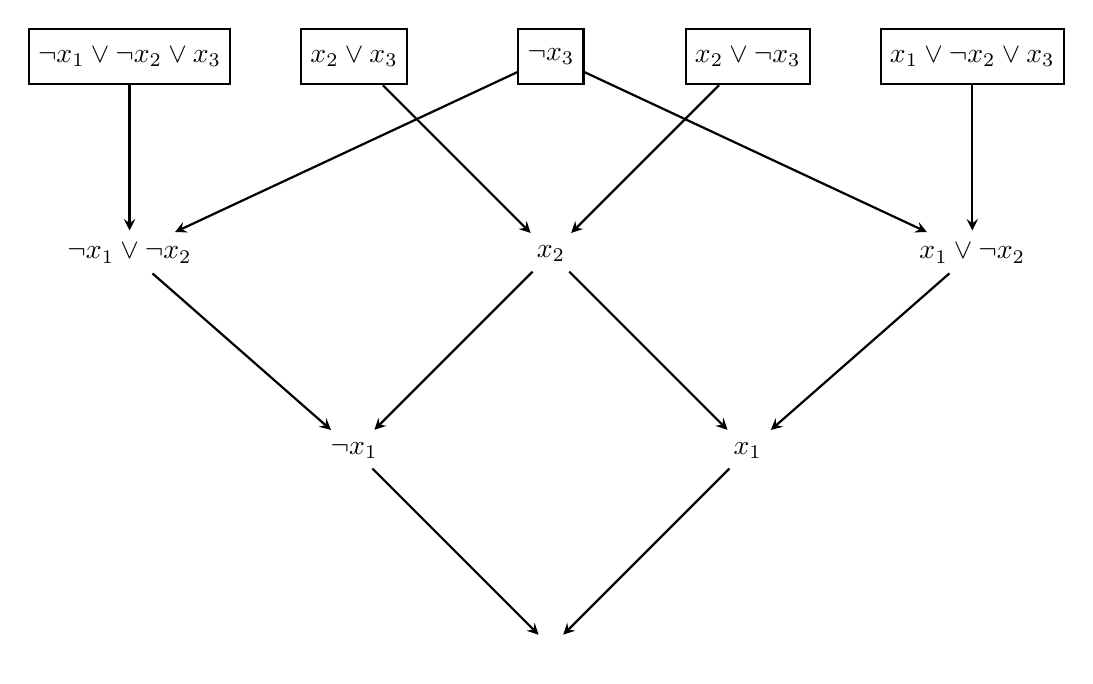
\begin{tikzpicture}[->,>=stealth,shorten >=1pt,auto,node distance=2.5cm, thick,main node/.style={scale=0.9,circle,draw,font=\sffamily\normalsize}]
            \node [rectangle, draw, minimum height=20](1) []{$\lnot{x_1} \lor \lnot{x_2} \lor x_3$};
            \node [rectangle, draw, minimum height=20](2) [right of=1, xshift = 10]{$x_2 \lor x_3$};
            \node [rectangle, draw, minimum height=20](3) [right of=2]{$\lnot{x_3}$};
            \node [rectangle, draw, minimum height=20](4) [right of=3]{$x_2 \lor \lnot{x_3}$};
            \node [rectangle, draw, minimum height=20](5) [right of=4, xshift = 10]{$x_1 \lor \lnot{x_2} \lor x_3$};

            \node (6) [below of=1]{$\lnot{x_1} \lor \lnot{x_2}$};
            \node (x) [below of=2]{};
            \node (7) [below of=3]{$x_2$};
            \node (y) [below of=4]{};
            \node (8) [below of=5]{$x_1 \lor \lnot{x_2}$};

            \node (9) [below of=x]{$\lnot{x_1}$};
            \node (10) [below of=y]{$x_1$};
            \node (z) [below of=7]{};
            
            \node (11) [below of=z]{$\square$};
        
            \path[every node/.style={font=\sffamily\small}]
                (1) edge (6)
                (2) edge (7)
                (3) edge (6)
                (3) edge (8)
                (4) edge (7)
                (5) edge (8)

                (6) edge (9)
                (7) edge (9)
                (7) edge (10)
                (8) edge (10)

                (9) edge (11)
                (10) edge (11)
                ;
        \end{tikzpicture}
        
        \caption{Rappresentazione grafica della precedente refutazione.}
    \end{figure}

    \begin{framedthm}{Completezza e correttezza della risoluzione}
        Il sistema di risoluzione è \textit{completo} e \textit{corretto}, ossia una formula CNF $F$ è insoddisfacibile se e solo se essa ha una una refutazione in risoluzione.
    \end{framedthm}

    \begin{proof} Omessa \end{proof}

    Osserviamo che il lemma di risoluzione permette di eliminare \underline{un solo letterale} alla volta e non tutti i letterali di segno opposto tra due clausole. Tuttavia, le due clausole $C$ e $D$ potrebbero contenere più di un letterale di segno opposto. Viene quindi naturale chiedersi cosa accada nel caso in cui venga applicata la regola di risoluzione in tale caso. Ad esempio, date le clausole $(x_1 \lor x_2 \lor \lnot x_3)$ e $(x_1 \lor \lnot x_2 \lor \lnot x_3)$, applicando il lemma di risoluzione su $x_2$ (o su $x_3$) abbiamo che:
    \[(x_1 \lor x_2 \lor \lnot x_3), (x_1 \lor \lnot x_2 \lor \lnot x_3) \models (x_1 \lor \lnot x_3) \lor (x_1 \lor x_3) \equiv 1\]

    In altre parole, applicare il lemma di risoluzione su tali clausole risulta essere del tutto \underline{inutile} poiché la clausola $1$ derivata non può essere usata per alcuna successiva risoluzione. Per tanto, quando tale casistica si verifica, è necessario procedere con altre combinazioni di clausole.

    Il precedente teorema implica che se una formula è soddisfacibile allora non può esistere una refutazione per essa. Per tanto, possiamo definire il seguente algoritmo basato sul lemma di risoluzione.

    \begin{algorithm}
        \caption{Algoritmo di risoluzione}
        \textbf{Input:} una formula CNF $F$ rappresentata come un insieme di clausole

        \textbf{Output:} True se la formula è insoddisfacibile, False altrimenti
        \begin{algorithmic}[1]
            \Function{risoluzione}{$F$}
                \While{$\exists (C \lor \ell), (D \lor \lnot{\ell}) \in F$ tali che $(C \lor D) \notin F$}
                    \State $F \gets F \cup \{(C \lor D)\}$
                \EndWhile
                \If{$\square \in F$}
                    \State Return True
                \Else
                    \State Return False
                \EndIf
            \EndFunction
        \end{algorithmic}
    \end{algorithm}

    \begin{framedthm}{Correttezza dell'algoritmo}
        Data una formula CNF $F$, l'esecuzione di \textsc{risoluzione}$(F)$ ritorna True se e solo se $F$ è insoddisfacibile
    \end{framedthm}

    \begin{proof} Omessa \end{proof}

    Ovviamente, tale algoritmo risulta essere molto lento poiché ad ogni iterazione deve potenzialmente controllare ogni possibile coppia di clausole -- se all'interazione $i$ ci sono $k$ clausole in $F$, allora verranno effettuati massimo $\binom{k}{2}$ controlli. Per tanto, un computer richiederebbe troppo tempo per stabilire che una formula è insoddisfacibile tramite la risoluzione (abbiamo già accennato come non esistono al momento algoritmi che abbiano questa caratteristica).

\end{document}
